
%%%%%%%%%%%%%%%%%%%%%%%%%%%%%%%%%%%%%%%%%
% The Legrand Orange Book
% LaTeX Template
% Version 1.4 (12/4/14)
%
% This template has been downloaded from:
% http://www.LaTeXTemplates.com
%
% Original author:
% Mathias Legrand (legrand.mathias@gmail.com)
%
% License:
% CC BY-NC-SA 3.0 (http://creativecommons.org/licenses/by-nc-sa/3.0/)
%
% Compiling this template:
% This template uses biber for its bibliography and makeindex for its index.
% When you first open the template, compile it from the command line with the 
% commands below to make sure your LaTeX distribution is configured correctly:
%
% 1) pdflatex main
% 2) makeindex main.idx -s StyleInd.ist
% 3) biber main
% 4) pdflatex main x 2
%
% After this, when you wish to update the bibliography/index use the appropriate
% command above and make sure to compile with pdflatex several times 
% afterwards to propagate your changes to the document.
%
% This template also uses a number of packages which may need to be
% updated to the newest versions for the template to compile. It is strongly
% recommended you update your LaTeX distribution if you have any
% compilation errors.
%
% Important note:
% Chapter heading images should have a 2:1 width:height ratio,
% e.g. 920px width and 460px height.
%
%%%%%%%%%%%%%%%%%%%%%%%%%%%%%%%%%%%%%%%%%

%----------------------------------------------------------------------------------------
%	PACKAGES AND OTHER DOCUMENT CONFIGURATIONS
%----------------------------------------------------------------------------------------
\documentclass[10pt,fleqn]{book} % Default font size and left-justified equations
\usepackage{booktabs}
\usepackage[top=3cm,bottom=3cm,left=3.2cm,right=3.2cm,headsep=10pt,a4paper]{geometry} % Page margins orig
%\usepackage[top=3cm,bottom=2.5cm,left=2.7cm,right=2.7cm,headsep=10pt,a4paper]{geometry} % Page margins
\usepackage[all]{xy}
\xyoption{arc}
\usepackage{stackrel}
\usepackage{enumitem}
\usepackage{xcolor} % Required for specifying colors by name
%\definecolor{maincolor}{RGB}{243,102,25} % Define the orange color used for highlighting throughout the book
\definecolor{maincolor}{rgb}{0.01, 0.31, 0.59}  % Define the blueish color used for highlighting throughout the book

% Font Settings
\usepackage{avant} % Use the Avantgarde font for headings
%\usepackage{times} % Use the Times font for headings
\usepackage{mathptmx} % Use the Adobe Times Roman as the default text font together with math symbols from the Sym­bol, Chancery and Com­puter Modern fonts

\usepackage{microtype} % Slightly tweak font spacing for aesthetics
\usepackage[utf8]{inputenc} % Required for including letters with accents
\usepackage[T1]{fontenc} % Use 8-bit encoding that has 256 glyphs

% Bibliography
\usepackage[style=alphabetic,sorting=nyt,sortcites=true,autopunct=true,autolang=hyphen,hyperref=true,abbreviate=false,backref=true,backend=biber]{biblatex}
\addbibresource{bibliography.bib} % BibTeX bibliography file
\defbibheading{bibempty}{}

% Index
\usepackage{calc} % For simpler calculation - used for spacing the index letter headings correctly
\usepackage{makeidx} % Required to make an index
\makeindex % Tells LaTeX to create the files required for indexing

% Listings

\usepackage{listings} % Required for inserting code snippets
%\usepackage[usenames,dvipsnames]{color} % Required for specifying custom colors and referring to colors by name

\definecolor{DarkGreen}{rgb}{0.0,0.4,0.0} % Comment color
\definecolor{highlight}{RGB}{255,251,204} % Code highlight color

\lstdefinestyle{Style1}{ % Define a style for your code snippet, multiple definitions can be made if, for example, you wish to insert multiple code snippets using different programming languages into one document
language=Perl, % Detects keywords, comments, strings, functions, etc for the language specified
backgroundcolor=\color{highlight}, % Set the background color for the snippet - useful for highlighting
basicstyle=\footnotesize\ttfamily, % The default font size and style of the code
breakatwhitespace=false, % If true, only allows line breaks at white space
breaklines=true, % Automatic line breaking (prevents code from protruding outside the box)
captionpos=b, % Sets the caption position: b for bottom; t for top
commentstyle=\usefont{T1}{pcr}{m}{sl}\color{DarkGreen}, % Style of comments within the code - dark green courier font
deletekeywords={}, % If you want to delete any keywords from the current language separate them by commas
%escapeinside={\%}, % This allows you to escape to LaTeX using the character in the bracket
firstnumber=1, % Line numbers begin at line 1
frame=single, % Frame around the code box, value can be: none, leftline, topline, bottomline, lines, single, shadowbox
frameround=tttt, % Rounds the corners of the frame for the top left, top right, bottom left and bottom right positions
keywordstyle=\color{Blue}\bf, % Functions are bold and blue
morekeywords={}, % Add any functions no included by default here separated by commas
numbers=left, % Location of line numbers, can take the values of: none, left, right
numbersep=10pt, % Distance of line numbers from the code box
numberstyle=\tiny\color{Gray}, % Style used for line numbers
rulecolor=\color{black}, % Frame border color
showstringspaces=false, % Don't put marks in string spaces
showtabs=false, % Display tabs in the code as lines
stepnumber=5, % The step distance between line numbers, i.e. how often will lines be numbered
stringstyle=\color{Purple}, % Strings are purple
tabsize=2, % Number of spaces per tab in the code
}

% Create a command to cleanly insert a snippet with the style above anywhere in the document
\newcommand{\insertcode}[2]{\begin{itemize}\item[]\lstinputlisting[caption=#2,label=#1,style=Style1]{#1}\end{itemize}} % The first argument is the script location/filename and the second is a caption for the listing

%----------------------------------------------------------------------------------------

%----------------------------------------------------------------------------------------
%	VARIOUS REQUIRED PACKAGES
%----------------------------------------------------------------------------------------

\usepackage{titlesec} % Allows customization of titles

\usepackage{graphicx} % Required for including pictures
\graphicspath{{Pictures/}} % Specifies the directory where pictures are stored

\usepackage{tikz} % Required for drawing custom shapes

\usepackage[english]{babel} % English language/hyphenation

\usepackage{enumitem} % Customize lists
\setlist{nolistsep} % Reduce spacing between bullet points and numbered lists

\usepackage{booktabs} % Required for nicer horizontal rules in tables

\usepackage{eso-pic} % Required for specifying an image background in the title page

%----------------------------------------------------------------------------------------
%	MAIN TABLE OF CONTENTS
%----------------------------------------------------------------------------------------

\usepackage{titletoc} % Required for manipulating the table of contents

\contentsmargin{0cm} % Removes the default margin
% Chapter text styling
\titlecontents{chapter}[1.25cm] % Indentation
{\addvspace{15pt}\large\sffamily\bfseries} % Spacing and font options for chapters
{\color{maincolor!60}\contentslabel[\Large\thecontentslabel]{1.25cm}\color{maincolor}} % Chapter number
{}  
{\color{maincolor!60}\normalsize\sffamily\bfseries\;\titlerule*[.5pc]{.}\;\thecontentspage} % Page number
% Section text styling
\titlecontents{section}[1.25cm] % Indentation
{\addvspace{5pt}\sffamily\bfseries} % Spacing and font options for sections
{\contentslabel[\thecontentslabel]{1.25cm}} % Section number
{}
{\sffamily\hfill\color{black}\thecontentspage} % Page number
[]
% Subsection text styling
\titlecontents{subsection}[1.25cm] % Indentation
{\addvspace{1pt}\sffamily\small} % Spacing and font options for subsections
{\contentslabel[\thecontentslabel]{1.25cm}} % Subsection number
{}
{\sffamily\;\titlerule*[.5pc]{.}\;\thecontentspage} % Page number
[] 

%----------------------------------------------------------------------------------------
%	MINI TABLE OF CONTENTS IN CHAPTER HEADS
%----------------------------------------------------------------------------------------

% Section text styling
\titlecontents{lsection}[0em] % Indendating
{\footnotesize\sffamily} % Font settings
{}
{}
{}

% Subsection text styling
\titlecontents{lsubsection}[.5em] % Indentation
{\normalfont\footnotesize\sffamily} % Font settings
{}
{}
{}
 
%----------------------------------------------------------------------------------------
%	PAGE HEADERS
%----------------------------------------------------------------------------------------

\usepackage{fancyhdr} % Required for header and footer configuration

\pagestyle{fancy}
\renewcommand{\chaptermark}[1]{\markboth{\sffamily\normalsize\bfseries\chaptername\ \thechapter.\ #1}{}} % Chapter text font settings
\renewcommand{\sectionmark}[1]{\markright{\sffamily\normalsize\thesection\hspace{5pt}#1}{}} % Section text font settings
\fancyhf{} \fancyhead[LE,RO]{\sffamily\normalsize\thepage} % Font setting for the page number in the header
\fancyhead[LO]{\rightmark} % Print the nearest section name on the left side of odd pages
\fancyhead[RE]{\leftmark} % Print the current chapter name on the right side of even pages
\renewcommand{\headrulewidth}{0.5pt} % Width of the rule under the header
\addtolength{\headheight}{2.5pt} % Increase the spacing around the header slightly
\renewcommand{\footrulewidth}{0pt} % Removes the rule in the footer
\fancypagestyle{plain}{\fancyhead{}\renewcommand{\headrulewidth}{0pt}} % Style for when a plain pagestyle is specified

% Removes the header from odd empty pages at the end of chapters
\makeatletter
\renewcommand{\cleardoublepage}{
\clearpage\ifodd\c@page\else
\hbox{}
\vspace*{\fill}
\thispagestyle{empty}
\newpage
\fi}

%----------------------------------------------------------------------------------------
%	THEOREM STYLES
%----------------------------------------------------------------------------------------

\usepackage{amsmath,amsfonts,amssymb,amsthm} % For math equations, theorems, symbols, etc

\newcommand{\intoo}[2]{\mathopen{]}#1\,;#2\mathclose{[}}
\newcommand{\ud}{\mathop{\mathrm{{}d}}\mathopen{}}
\newcommand{\intff}[2]{\mathopen{[}#1\,;#2\mathclose{]}}

%%%%%%%%%%%%%%%%%%%%%%%%%%%%%%%%%%%%%%%%%%%%%%%%%%%%%%%%%%%%%%%%%%%%%%%%%%%
%%%%%%%%%%%%%%%%%%%% dedicated to boxed/framed environements %%%%%%%%%%%%%%
%%%%%%%%%%%%%%%%%%%%%%%%%%%%%%%%%%%%%%%%%%%%%%%%%%%%%%%%%%%%%%%%%%%%%%%%%%%
\newtheoremstyle{maincolornumbox}% % Theorem style name
{0pt}% Space above
{0pt}% Space below
{\normalfont}% % Body font
{}% Indent amount
{\small\bf\sffamily\color{maincolor}}% % Theorem head font
{\;}% Punctuation after theorem head
{0.25em}% Space after theorem head
{\small\sffamily\color{maincolor}\thmname{#1}\nobreakspace\thmnumber{\@ifnotempty{#1}{}\@upn{#2}}% Theorem text (e.g. Theorem 2.1)
\thmnote{\nobreakspace\the\thm@notefont\sffamily\bfseries\color{black}---\nobreakspace#3.}} % Optional theorem note
\renewcommand{\qedsymbol}{$\blacksquare$}% Optional qed square

\newtheoremstyle{blacknumex}% Theorem style name
{5pt}% Space above
{5pt}% Space below
{\normalfont}% Body font
{} % Indent amount
{\small\bf\sffamily}% Theorem head font
{\;}% Punctuation after theorem head
{0.25em}% Space after theorem head
{\small\sffamily{\tiny\ensuremath{\blacksquare}}\nobreakspace\thmname{#1}\nobreakspace\thmnumber{\@ifnotempty{#1}{}\@upn{#2}}% Theorem text (e.g. Theorem 2.1)
\thmnote{\nobreakspace\the\thm@notefont\sffamily\bfseries---\nobreakspace#3.}}% Optional theorem note

\newtheoremstyle{blacknumbox} % Theorem style name
{0pt}% Space above
{0pt}% Space below
{\normalfont}% Body font
{}% Indent amount
{\small\bf\sffamily}% Theorem head font
{\;}% Punctuation after theorem head
{0.25em}% Space after theorem head
{\small\sffamily\thmname{#1}\nobreakspace\thmnumber{\@ifnotempty{#1}{}\@upn{#2}}% Theorem text (e.g. Theorem 2.1)
\thmnote{\nobreakspace\the\thm@notefont\sffamily\bfseries---\nobreakspace#3.}}% Optional theorem note

%%%%%%%%%%%%%%%%%%%%%%%%%%%%%%%%%%%%%%%%%%%%%%%%%%%%%%%%%%%%%%%%%%%%%%%%%%%
%%%%%%%%%%%%% dedicated to non-boxed/non-framed environements %%%%%%%%%%%%%
%%%%%%%%%%%%%%%%%%%%%%%%%%%%%%%%%%%%%%%%%%%%%%%%%%%%%%%%%%%%%%%%%%%%%%%%%%%
\newtheoremstyle{maincolornum}% % Theorem style name
{5pt}% Space above
{5pt}% Space below
{\normalfont}% % Body font
{}% Indent amount
{\small\bf\sffamily\color{maincolor}}% % Theorem head font
{\;}% Punctuation after theorem head
{0.25em}% Space after theorem head
{\small\sffamily\color{maincolor}\thmname{#1}\nobreakspace\thmnumber{\@ifnotempty{#1}{}\@upn{#2}}% Theorem text (e.g. Theorem 2.1)
\thmnote{\nobreakspace\the\thm@notefont\sffamily\bfseries\color{black}---\nobreakspace#3.}} % Optional theorem note
\renewcommand{\qedsymbol}{$\blacksquare$}% Optional qed square
\makeatother

% Defines the theorem text style for each type of theorem to one of the three styles above
\newcounter{dummy} 
\numberwithin{dummy}{section}
\theoremstyle{maincolornumbox}
\newtheorem{theoremeT}[dummy]{Theorem}
\newtheorem{propositionT}[dummy]{Proposition}
\newtheorem{conjectureT}[dummy]{Conjecture}
\newtheorem{lemmaT}[dummy]{Lemma}
\newtheorem{corollaryT}[dummy]{Corollary}
\newtheorem{problem}{Problem}[chapter]
\newtheorem{exerciseT}{Exercise}[chapter]
\theoremstyle{blacknumex}
\newtheorem{exampleT}{Example}[chapter]
\theoremstyle{blacknumbox}
\newtheorem{vocabulary}{Vocabulary}[chapter]
\newtheorem{definitionT}{Definition}[section]
\theoremstyle{maincolornum}


%----------------------------------------------------------------------------------------
%	DEFINITION OF COLORED BOXES
%----------------------------------------------------------------------------------------

\RequirePackage[framemethod=default]{mdframed} % Required for creating the theorem, definition, exercise and corollary boxes

% Theorem box
\newmdenv[skipabove=7pt,
skipbelow=7pt,
backgroundcolor=black!5,
linecolor=maincolor,
innerleftmargin=5pt,
innerrightmargin=5pt,
innertopmargin=5pt,
leftmargin=0cm,
rightmargin=0cm,
innerbottommargin=5pt]{tBox}

% Exercise box	  
\newmdenv[skipabove=7pt,
skipbelow=7pt,
rightline=false,
leftline=true,
topline=false,
bottomline=false,
backgroundcolor=maincolor!10,
linecolor=maincolor,
innerleftmargin=5pt,
innerrightmargin=5pt,
innertopmargin=5pt,
innerbottommargin=5pt,
leftmargin=0cm,
rightmargin=0cm,
linewidth=4pt]{eBox}	

% Definition box
\newmdenv[skipabove=7pt,
skipbelow=7pt,
rightline=false,
leftline=true,
topline=false,
bottomline=false,
linecolor=maincolor,
innerleftmargin=5pt,
innerrightmargin=5pt,
innertopmargin=0pt,
leftmargin=0cm,
rightmargin=0cm,
linewidth=4pt,
innerbottommargin=0pt]{dBox}	

% Corollary box
\newmdenv[skipabove=7pt,
skipbelow=7pt,
rightline=false,
leftline=true,
topline=false,
bottomline=false,
linecolor=gray,
backgroundcolor=black!5,
innerleftmargin=5pt,
innerrightmargin=5pt,
innertopmargin=5pt,
leftmargin=0cm,
rightmargin=0cm,
linewidth=4pt,
innerbottommargin=5pt]{cBox}

% Creates an environment for each type of theorem and assigns it a theorem text style from the "Theorem Styles" section above and a colored box from above
\newenvironment{theorem}{\begin{tBox}\begin{theoremeT}}{\end{theoremeT}\end{tBox}}
\newenvironment{conjecture}{\begin{tBox}\begin{conjectureT}}{\end{conjectureT}\end{tBox}}
\newenvironment{proposition}{\begin{tBox}\begin{propositionT}}{\end{propositionT}\end{tBox}}
\newenvironment{exercise}{\begin{eBox}\begin{exerciseT}}{\hfill{\color{maincolor}\tiny\ensuremath{\blacksquare}}\end{exerciseT}\end{eBox}}				  
\newenvironment{definition}{\begin{dBox}\begin{definitionT}}{\end{definitionT}\end{dBox}}	
\newenvironment{example}{\begin{exampleT}}{\hfill{\tiny\ensuremath{\blacksquare}}\end{exampleT}}		
\newenvironment{corollary}{\begin{cBox}\begin{corollaryT}}{\end{corollaryT}\end{cBox}}	
\newenvironment{lemma}{\begin{cBox}\begin{lemmaT}}{\end{lemmaT}\end{cBox}}	

%----------------------------------------------------------------------------------------
%	REMARK ENVIRONMENT
%----------------------------------------------------------------------------------------

\newenvironment{remark}{\par\vspace{10pt}\small % Vertical white space above the remark and smaller font size
\begin{list}{}{
\leftmargin=35pt % Indentation on the left
\rightmargin=25pt}\item\ignorespaces % Indentation on the right
\makebox[-2.5pt]{\begin{tikzpicture}[overlay]
\node[draw=maincolor!60,line width=1pt,circle,fill=maincolor!25,font=\sffamily\bfseries,inner sep=2pt,outer sep=0pt] at (-15pt,0pt){\textcolor{maincolor}{R}};\end{tikzpicture}} % Orange R in a circle
\advance\baselineskip -1pt}{\end{list}\vskip5pt} % Tighter line spacing and white space after remark

%----------------------------------------------------------------------------------------
%	SECTION NUMBERING IN THE MARGIN
%----------------------------------------------------------------------------------------

\makeatletter
\renewcommand{\@seccntformat}[1]{\llap{\textcolor{maincolor}{\csname the#1\endcsname}\hspace{1em}}}                    
\renewcommand{\section}{\@startsection{section}{1}{\z@}
{-4ex \@plus -1ex \@minus -.4ex}
{1ex \@plus.2ex }
{\normalfont\large\sffamily\bfseries}}
\renewcommand{\subsection}{\@startsection {subsection}{2}{\z@}
{-3ex \@plus -0.1ex \@minus -.4ex}
{0.5ex \@plus.2ex }
{\normalfont\sffamily\bfseries}}
\renewcommand{\subsubsection}{\@startsection {subsubsection}{3}{\z@}
{-2ex \@plus -0.1ex \@minus -.2ex}
{.2ex \@plus.2ex }
{\normalfont\small\sffamily\bfseries}}                        
\renewcommand\paragraph{\@startsection{paragraph}{4}{\z@}
{-2ex \@plus-.2ex \@minus .2ex}
{.1ex}
{\normalfont\small\sffamily\bfseries}}

%----------------------------------------------------------------------------------------
%	HYPERLINKS IN THE DOCUMENTS
%----------------------------------------------------------------------------------------

% For an unclear reason, the package should be loaded now and not later
\usepackage{hyperref}
\hypersetup{hidelinks,colorlinks=false,breaklinks=true,urlcolor= maincolor,bookmarksopen=false,pdftitle={Title},pdfauthor={Author}}

%----------------------------------------------------------------------------------------
%	CHAPTER HEADINGS
%----------------------------------------------------------------------------------------

% The set-up below should be (sadly) manually adapted to the overall margin page septup controlled by the geometry package loaded in the main.tex document. It is possible to implement below the dimensions used in the goemetry package (top,bottom,left,right)... TO BE DONE

\newcommand{\thechapterimage}{}
\newcommand{\chapterimage}[1]{\renewcommand{\thechapterimage}{#1}}

% Numbered chapters with mini tableofcontents
\def\thechapter{\arabic{chapter}}
\def\@makechapterhead#1{
\thispagestyle{empty}
{\centering \normalfont\sffamily
\ifnum \c@secnumdepth >\m@ne
\if@mainmatter
\startcontents
\begin{tikzpicture}[remember picture,overlay]
\node at (current page.north west)
{\begin{tikzpicture}[remember picture,overlay]
\node[anchor=north west,inner sep=0pt] at (0,0) {\includegraphics[width=\paperwidth]{\thechapterimage}};
%%%%%%%%%%%%%%%%%%%%%%%%%%%%%%%%%%%%%%%%%%%%%%%%%%%%%%%%%%%%%%%%%%%%%%%%%%%%%%%%%%%%%
% Commenting the 3 lines below removes the small contents box in the chapter heading
\fill[color=maincolor!10!white,opacity=.6] (1cm,0) rectangle (8cm,-7cm);
\node[anchor=north west] at (1.1cm,-.35cm) {\parbox[t][8cm][t]{6.5cm}{\huge\bfseries\flushleft \printcontents{l}{1}{\setcounter{tocdepth}{2}}}};
\draw[anchor=west] (5cm,-9cm) node [rounded corners=20pt,fill=maincolor!10!white,text opacity=1,draw=maincolor,draw opacity=1,line width=1.5pt,fill opacity=.6,inner sep=12pt]{\huge\sffamily\bfseries\textcolor{black}{\thechapter. #1\strut\makebox[22cm]{}}};
%%%%%%%%%%%%%%%%%%%%%%%%%%%%%%%%%%%%%%%%%%%%%%%%%%%%%%%%%%%%%%%%%%%%%%%%%%%%%%%%%%%%%
\end{tikzpicture}};
\end{tikzpicture}}
\par\vspace*{230\p@}
\fi
\fi}

% Unnumbered chapters without mini tableofcontents (could be added though) 
\def\@makeschapterhead#1{
\thispagestyle{empty}
{\centering \normalfont\sffamily
\ifnum \c@secnumdepth >\m@ne
\if@mainmatter
\begin{tikzpicture}[remember picture,overlay]
\node at (current page.north west)
{\begin{tikzpicture}[remember picture,overlay]
\node[anchor=north west,inner sep=0pt] at (0,0) {\includegraphics[width=\paperwidth]{\thechapterimage}};
\draw[anchor=west] (5cm,-9cm) node [rounded corners=20pt,fill=maincolor!10!white,fill opacity=.6,inner sep=12pt,text opacity=1,draw=maincolor,draw opacity=1,line width=1.5pt]{\huge\sffamily\bfseries\textcolor{black}{#1\strut\makebox[22cm]{}}};
\end{tikzpicture}};
\end{tikzpicture}}
\par\vspace*{230\p@}
\fi
\fi
}
\makeatother

%Blackboard Letters
\newcommand{\bbQ}{\mathbb{Q}}
\newcommand{\bbI}{\mathbb{I}}
\newcommand{\bbL}{\mathbb{L}}
\newcommand{\bbF}{\mathbb{F}}
\newcommand{\bbC}{\mathbb{C}}
\newcommand{\bbD}{\mathbb{D}}
\newcommand{\bbZ}{\mathbb{Z}}
\newcommand{\bbP}{\mathbb{P}}
\newcommand{\bbA}{\mathbb{A}}
\newcommand{\bbB}{\mathbb{B}}
\newcommand{\bbR}{\mathbb{R}}
\newcommand{\bbG}{\mathbb{G}}
\newcommand{\bbE}{\mathbb{E}}
\newcommand{\bbH}{\mathbb{H}}
\newcommand{\bbN}{\mathbb{N}}
\newcommand{\bbT}{\mathbb{T}}
\newcommand{\bbW}{\mathbb{W}}
\newcommand{\bbV}{\mathbb{V}}

%Bold Letters 
\newcommand{\bQ}{\mathbf{Q}}
\newcommand{\bF}{\mathbf{F}}
\newcommand{\bC}{\mathbf{C}}
\newcommand{\bJ}{\mathbf{J}}
\newcommand{\bZ}{\mathbf{Z}}
\newcommand{\bP}{\mathbf{P}}
\newcommand{\bA}{\mathbf{A}}
\newcommand{\bR}{\mathbf{R}}
\newcommand{\bG}{\mathbf{G}}
\newcommand{\bE}{\mathbf{E}}
\newcommand{\bH}{\mathbf{H}}
\newcommand{\bN}{\mathbf{N}}

%(for Q,R,N,C,...)
\renewcommand{\AA}{\bbA}
\newcommand{\BB}{\bbB}
\newcommand{\DD}{\bbD}
\newcommand{\QQ}{\bbQ}
\newcommand{\II}{\bbI}
\newcommand{\WW}{\bbW}
\newcommand{\RR}{\bbR}
\newcommand{\CC}{\bbC}
\newcommand{\VV}{\bbV}
\newcommand{\FF}{\bbF}
\newcommand{\HH}{\bbH}
\newcommand{\ZZ}{\bbZ}
\newcommand{\NN}{\bbN}
\newcommand{\PP}{\bbP}

\newcommand{\Qbar}{\overline{\QQ}}

%Caligraphic (Sheaves...)
\newcommand{\cA}{\mathcal{A}}
\newcommand{\cB}{\mathcal{B}}
\newcommand{\cC}{\mathcal{C}}
\newcommand{\cD}{\mathcal{D}}
\newcommand{\cO}{\mathcal{O}}
\newcommand{\cF}{\mathcal{F}}
\newcommand{\cG}{\mathcal{G}}
\newcommand{\cI}{\mathcal{I}}
\newcommand{\cJ}{\mathcal{J}}
\newcommand{\cL}{\mathcal{L}}
\newcommand{\cH}{\mathcal{H}}
\newcommand{\chh}{\mathcal{h}}
\newcommand{\cR}{\mathcal{R}}
\newcommand{\cM}{\mathcal{M}}
\newcommand{\cN}{\mathcal{N}}
\newcommand{\cE}{\mathcal{E}}
\newcommand{\cP}{\mathcal{P}}
\newcommand{\cT}{\mathcal{T}}
\newcommand{\cU}{\mathcal{U}}
\newcommand{\cV}{\mathcal{V}}
\newcommand{\cW}{\mathcal{W}}
\newcommand{\cZ}{\mathcal{Z}}

\newcommand{\cHom}{\operatorname{\mathcal{H}om}}
\newcommand{\shomega}{\underline{\omega}}

%Category names
\newcommand{\AbGrp}{\textbf{Ab}}
\newcommand{\Ab}{\AbGrp}
\newcommand{\Sheaves}{\textbf{Sheaves}}
\newcommand{\Rings}{\textbf{Rings}}
\newcommand{\Mod}{\textbf{Mod}}
\newcommand{\Sh}{\textbf{Sh}}
\newcommand{\Sch}{\textbf{Sch}}
\newcommand{\Sets}{\textbf{Sets}}
\newcommand{\Mot}{\textbf{Mot}}

%Fraktor letters, eg naming ideals

\newcommand{\fA}{\mathfrak A}
\newcommand{\fR}{\mathfrak R}
\newcommand{\fp}{\mathfrak p}
\newcommand{\fq}{\mathfrak q}
\newcommand{\fP}{\mathfrak P}
\newcommand{\fQ}{\mathfrak Q}
\newcommand{\fa}{\mathfrak a}
\newcommand{\fb}{\mathfrak b}
\newcommand{\fc}{\mathfrak c}
\newcommand{\fd}{\mathfrak d}
\newcommand{\fm}{\mathfrak m}
\newcommand{\fn}{\mathfrak n}
\newcommand{\fo}{\mathfrak o}
\newcommand{\fS}{\mathfrak S}
\newcommand{\fN}{\mathfrak N}
\newcommand{\fU}{\mathfrak U}
\newcommand{\fX}{\mathfrak X}
\newcommand{\fY}{\mathfrak Y}

\def\wh{\widehat}

%Some common math operators
\DeclareMathOperator{\order}{ord}
\DeclareMathOperator{\covol}{covol}
\DeclareMathOperator{\Inf}{Inf}
\DeclareMathOperator{\Cris}{Cris}
% \DeclareMathOperator{\Sh}{Sh}
\DeclareMathOperator{\val}{val}
\DeclareMathOperator{\Ram}{Ram}
\DeclareMathOperator{\Stab}{Stab}
\DeclareMathOperator{\St}{St}
\DeclareMathOperator{\sgn}{sgn}
\DeclareMathOperator{\rk}{rk}
\DeclareMathOperator{\cork}{cork}
\DeclareMathOperator{\lcm}{lcm}
\DeclareMathOperator{\Gal}{Gal}
\DeclareMathOperator{\Spec}{Spec}
\DeclareMathOperator{\Max}{Max}
\DeclareMathOperator{\Sp}{Sp}
\DeclareMathOperator{\Mp}{Mp}
\DeclareMathOperator{\Spf}{Spf}
\DeclareMathOperator{\Proj}{Proj}
\DeclareMathOperator{\Jacobson}{\mathfrak J}
\DeclareMathOperator{\Nilradical}{\mathfrak N}
\DeclareMathOperator{\rad}{\mathfrak{rad}}
\DeclareMathOperator{\Hom}{Hom}
\DeclareMathOperator{\End}{End}
\DeclareMathOperator{\Aut}{Aut}
\DeclareMathOperator{\Isom}{Isom}
\DeclareMathOperator{\car}{char}
\DeclareMathOperator{\gl}{GL}
\DeclareMathOperator{\GL}{GL}
\DeclareMathOperator{\PGL}{PGL}
\DeclareMathOperator{\tr}{Tr}
\DeclareMathOperator{\disc}{disc}
\DeclareMathOperator{\discrd}{discrd}
\DeclareMathOperator{\supp}{Supp}
\DeclareMathOperator{\Div}{Div}
\DeclareMathOperator{\Pic}{Pic}
\DeclareMathOperator{\divv}{div}
%\DeclareMathOperator{\ord}{ord}
\DeclareMathOperator{\res}{Res}
\DeclareMathOperator{\coker}{coker}
\DeclareMathOperator{\img}{img}
\DeclareMathOperator{\Tate}{Tate}
\DeclareMathOperator{\gr}{gr}
\DeclareMathOperator{\Tot}{Tot}
\DeclareMathOperator{\Tor}{Tor}
\DeclareMathOperator{\sym}{Sym}
\DeclareMathOperator{\ev}{ev}
\DeclareMathOperator{\Symm}{Symm}
\DeclareMathOperator{\Ann}{Ann}
\DeclareMathOperator{\length}{length}
\DeclareMathOperator{\dlog}{dlog}
\DeclareMathOperator{\chow}{CH}
\DeclareMathOperator{\cl}{cl}
\DeclareMathOperator{\Cl}{Cl}
\DeclareMathOperator{\AJ}{AJ}
\DeclareMathOperator{\Ext}{Ext}
\DeclareMathOperator{\Sym}{Sym}
\DeclareMathOperator{\Nm}{Nm}
\DeclareMathOperator{\nrd}{Nrd}
\DeclareMathOperator{\trd}{trd}
\DeclareMathOperator{\Corr}{Corr}
\DeclareMathOperator{\pr}{pr}
\DeclareMathOperator{\SL}{SL}
\DeclareMathOperator{\PSL}{PSL}
\DeclareMathOperator{\SO}{SO}
\DeclareMathOperator{\SU}{SU}
\DeclareMathOperator{\Graph}{Graph}
\DeclareMathOperator{\Fil}{Fil}
\DeclareMathOperator{\red}{red}
\DeclareMathOperator{\MF}{MF}
\DeclareMathOperator{\Rep}{Rep}
\DeclareMathOperator{\Reg}{Reg}
\DeclareMathOperator{\Frac}{Frac}
\DeclareMathOperator{\Dst}{D_{\st}}
\DeclareMathOperator{\Vst}{V_{\st}}
\DeclareMathOperator{\NS}{NS}
\DeclareMathOperator{\ad}{ad}
\DeclareMathOperator{\stab}{stab}
\DeclareMathOperator{\Gr}{Gr}
\DeclareMathOperator{\Frob}{Frob}
\DeclareMathOperator{\cond}{cond}
\DeclareMathOperator{\Sel}{Sel}
\DeclareMathOperator{\Ind}{Ind}
\DeclareMathOperator{\cInd}{c-Ind}
\def\det{\operatorname{det}}
\DeclareMathOperator{\diag}{diag}
\DeclareMathOperator{\Alb}{Alb}
\DeclareMathOperator{\Jet}{Jet}
\DeclareMathOperator{\Lie}{Lie}
\DeclareMathOperator{\Coh}{Coh}
\DeclareMathOperator{\QCoh}{QCoh}
\DeclareMathOperator{\tors}{tors}

%\DeclareSymbolFont{cyrletters}{OT2}{wncyr}{m}{n}
%\DeclareMathSymbol{\Sha}{\mathalpha}{cyrletters}{"58}

%Some common abreviations
\newcommand{\lto}{\longrightarrow}
\newcommand{\dfn}{\ensuremath{{:=}}}
\newcommand{\nfd}{\ensuremath{{=:}}}
\newcommand{\surjects}{\twoheadrightarrow}
\newcommand{\injects}{\hookrightarrow}
\newcommand{\id}{\ensuremath \text{Id}}
\newcommand{\tns}[1][]{\otimes_{\!#1}}
\newcommand{\mtx}[4]{\left(\begin{matrix}#1&#2\\#3&#4\end{matrix}\right)}
\newcommand{\mat}[1]{\left(\begin{matrix}#1\end{matrix}\right)}
\newcommand{\smat}[1]{\left(\begin{smallmatrix}#1\end{smallmatrix}\right)}
\newcommand{\smtx}[4]{\left(\begin{smallmatrix}#1&#2\\#3&#4\end{smallmatrix}\right)}
\newcommand{\slz}{\operatorname{SL}_2(\ZZ)}

\newcommand{\emphh}[2][ ]{%
\ifthenelse{\equal{#1}{ }}{\index{#2} {\emph{#2}}}{\index{#1@#2} {\emph{#2}}}%
}

%\def\emphh{\emph}

\def\sumprime{\mathop{\sum{\raise3pt\hbox{${}'$}}}} %Copied from somewhere else...
\def\prodprime{\mathop{\prod{\raise3pt\hbox{${}'$}}}} %Copied from somewhere else...

\newcommand{\et}{{\text{et}}}
\newcommand{\dR}{{\text{dR}}}
\newcommand{\cont}{{\text{cont}}}
\newcommand{\cris}{{\text{cris}}}
\newcommand{\Het}{H_\et}
\newcommand{\Hdr}{H_\dR}
\newcommand{\Hcris}{H_\cris}
\newcommand{\Bcris}{B_\cris}
\newcommand{\Dcris}{D_\cris}
\newcommand{\Vcris}{V_\cris}
\newcommand{\cHdr}{\cH_\dR}
\newcommand{\Hcont}{H_\cont}
\newcommand{\Hst}{H_\st}
\newcommand{\Char}{C_{\text{har}}}
\newcommand{\frob}{{\text{frob}}}
\newcommand{\hol}{{\text{hol}}}
\newcommand{\sm}{{\text{sm}}}
\newcommand{\usm}{{\text{usm}}}
\newcommand{\llangle}{\langle\!\langle}
\newcommand{\rrangle}{\rangle\!\rangle}

\newcommand{\poinc}[2]{\langle{#1},{#2}\rangle_{\text{Poinc}}}

\newcommand{\bbl}{[\hspace{-1.5pt}[}
\newcommand{\bbr}{]\hspace{-1.5pt}]}
\newcommand{\pseries}[2]{{#1}\bbl {#2}\bbr}

\newcommand{\Oneforms}[2]{\ensuremath\Omega_{\cO_{#1}/\cO_{#2}}}
\newcommand{\eps}{\varepsilon}
\newcommand{\mmu}{\mu\!\!\!\mu}
\newcommand{\Rmax}{{\cR^{\text{max}}}}
\newcommand{\an}{\text{an}}
\newcommand{\ur}{\text{ur}}
\newcommand{\barrr}{\overline}

\newcommand{\st}{\text{st}}
\newcommand{\Bst}{B_{\st}}

\newcommand{\tto}[1]{%
\ifthenelse{\equal{#1}{}}{\to}{\stackrel{#1}{\to}}}

\newcommand{\abs}[1]{|{#1}|}
\newcommand{\fabs}[1]{\|{#1}\|}

%Commands for fast typesetting
\newcommand{\nc}[2]{\newcommand{#1}{#2}}
\newcommand{\on}[2]{\operatorname{#1}{#2}}


\newcommand{\ol}[1]{\overline{#1}}
\newcommand{\ul}[1]{\underline{#1}}
\newcommand{\dr}{\text{dR}}
\newcommand{\Bdr}{{B_{\dr}}}
\newcommand{\Ddr}{{D_{\dr}}}
\newcommand{\Dsen}{{D_{\text{sen}}}}
\newcommand{\ab}{\text{ab}}
\newcommand{\HT}{\text{HT}}
\newcommand{\Bht}{{B_{\HT}}}
\newcommand{\repzpgamma}{\Rep_{\ZZ_p}(\Gamma)}
\newcommand{\repqpgamma}{\Rep_{\QQ_p}(\Gamma)}
\newcommand{\Dht}{{D_{\HT}}}
\renewcommand{\Vec}{\text{Vec}}
\newcommand{\EtPhiMod}[1][E]{{\phi M_{#1}^{\et}}}
\newcommand{\cOE}{{\cO_\cE}}
\newcommand{\hodge}{\text{Hodge}}
\newcommand{\ock}{\cO_{\CC_K}}
\newcommand{\ses}[4][]{ #1 #2\to #1 #3\to #1 #4 }
\newcommand{\wa}{{\text{wa}}}
\newcommand{\aR}{{\fA\fR}}
\newcommand{\Aug}{{\fA u g }}
\newcommand{\bOne}{{1\!\!1}}
\newcommand{\Wedge}{\Lambda}
\newcommand{\ord}{{\text{ord}}}
\newcommand{\can}{{\text{can}}}
\newcommand{\crit}{{\text{crit}}}
\renewcommand{\ss}{{\text{ss}}}
\newcommand{\bbf}{{\mathbbm{f}}}
\newcommand{\hecke}{{\mathfrak h}}
\newcommand{\Hecke}{{\mathfrak H}}

%For warnings (editing)
%\makeindex{fixmes}
%\newcommand{\fixme}[1]{}
\newcommand{\fixme}[1]{\footnote{\textbf{ FIXME: } \textrm{#1}}}

%%% Local Variables: 
%%% mode: latex
%%% TeX-master: "main"
%%% End: 
 % Insert the commands.tex file which contains the majority of the structure behind the template
\setcounter{tocdepth}{1}

%----------------------------------------------------------------------------------------
%	HIDE BLOCKS OF TEXT
%----------------------------------------------------------------------------------------

\usepackage{expl3,xparse}
\ExplSyntaxOn
\box_new:N \l_mypkg_box
\int_new:N \l_mypkg_cleanup_int
\DeclareDocumentCommand{\hideit}{O{1}+m}
  {
    \tex_setbox:D \l_mypkg_box \tex_vbox:D
      {
        #2\par
        \dim_zero:N \tex_baselineskip:D
        \dim_zero:N \tex_lineskip:D
        \dim_zero:N \tex_lineskiplimit:D
        \int_set:Nn \l_mypkg_cleanup_int {#1}
        \mypkg_dismantle_loop:
      }
    \tex_unvbox:D \l_mypkg_box
  }
\cs_new_protected:Npn \mypkg_dismantle_loop:
  {
    \prg_replicate:nn { \l_mypkg_cleanup_int }
      {
        \skip_if_eq:nnT { \tex_lastskip:D } { \c_zero_skip } { \tex_unskip:D }
        \dim_compare:nT { \tex_lastkern:D = \c_zero_dim } { \tex_unkern:D }
        \int_compare:nT { \tex_lastpenalty:D = \c_zero } { \tex_unpenalty:D }
      }
    \skip_if_eq:nnTF { \tex_lastskip:D } { \c_zero_skip }
      {
        \dim_compare:nTF { \tex_lastkern:D = \c_zero_dim }
          {
            \int_compare:nTF { \tex_lastpenalty:D = \c_zero }
              {
                \box_set_to_last:N \l_mypkg_box
                \box_if_empty:NF \l_mypkg_box
                  { \mypkg_dismantle_box: }
              }
              { \mypkg_dismantle_penalty: }
          }
          { \mypkg_dismantle_kern: }
      }
      { \mypkg_dismantle_skip: }
  }
\cs_new_protected:Npn \mypkg_dismantle_skip:
  { \mypkg_dismantle_aux:nN { \tex_vskip:D \skip_use:N \tex_lastskip:D } \tex_unskip:D }
\cs_new_protected:Npn \mypkg_dismantle_kern:
  { \mypkg_dismantle_aux:nN { \tex_kern:D \dim_use:N \tex_lastkern:D } \tex_unkern:D }
\cs_new_protected:Npn \mypkg_dismantle_penalty:
  { \mypkg_dismantle_aux:nN { \tex_penalty:D \int_use:N \tex_lastpenalty:D } \tex_unpenalty:D }
\cs_new_protected:Npn \mypkg_dismantle_box:
  { \mypkg_dismantle_aux:nN { \tex_vbox:D to \dim_eval:n { \box_ht:N \l_mypkg_box + \box_dp:N \l_mypkg_box } { } } \scan_stop: }
\cs_new_protected:Npn \mypkg_dismantle_aux:nN #1#2
  {
    \use:x
      {
        #2
        \mypkg_dismantle_loop:
        #1 \scan_stop:
      }
  }
\ExplSyntaxOff

\newenvironment{hiddenproof}{\textbf{Assigned exercise}\begin{proof}\hideit\{}{\}\end{proof}}

\begin{document}

%----------------------------------------------------------------------------------------
%	TITLE PAGE
%----------------------------------------------------------------------------------------

\begingroup
\thispagestyle{empty}
\AddToShipoutPicture*{\put(6,5){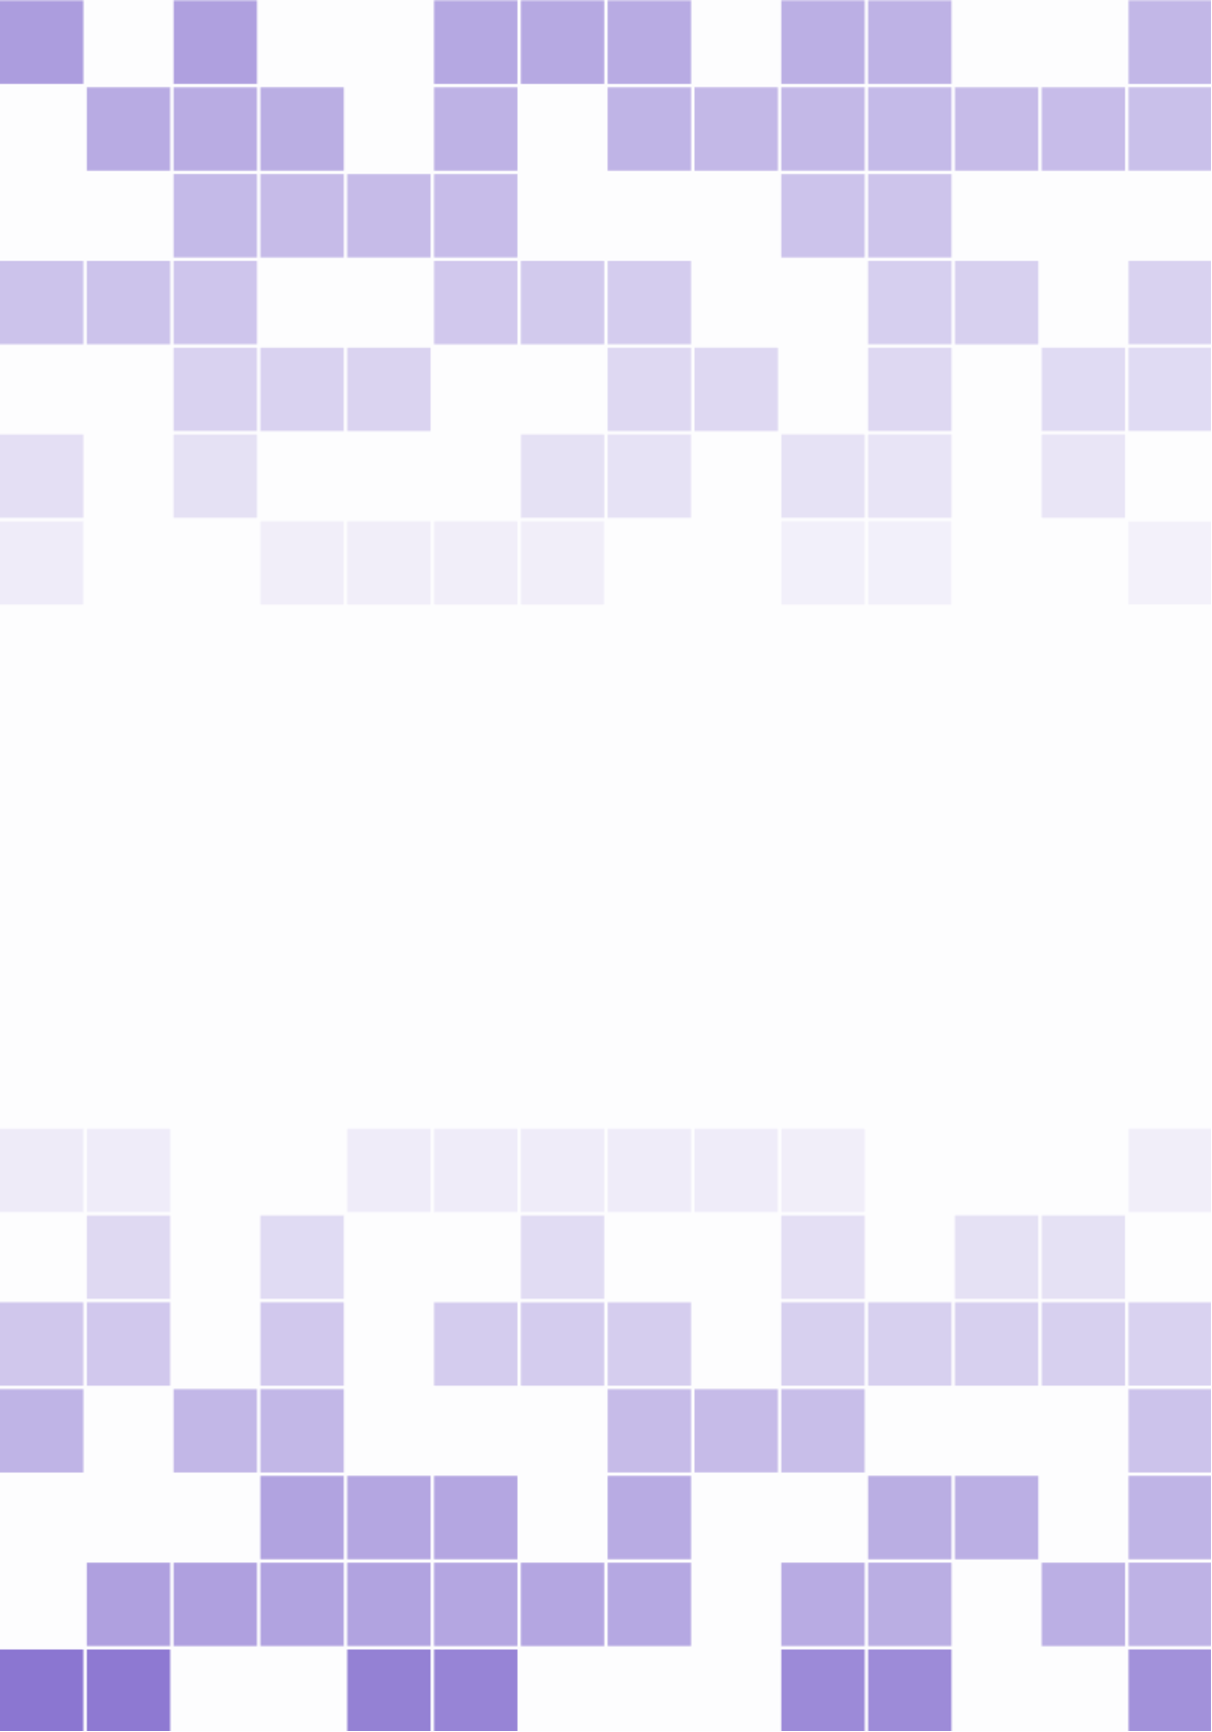
\includegraphics[scale=1]{background}}} % Image background
\centering
\vspace*{9cm}
\par\normalfont\fontsize{35}{35}\sffamily\selectfont
Modular Forms (MA4H9)\par % Book title
\vspace*{1cm}
{\Huge Marc Masdeu}\par % Author name
{\small\url{http://www.warwick.ac.uk/mmasdeu/}}\par
\endgroup

%----------------------------------------------------------------------------------------
%	COPYRIGHT PAGE
%----------------------------------------------------------------------------------------

\newpage
~\vfill
\thispagestyle{empty}

\noindent Copyright \copyright\ 2015 Marc Masdeu\\ % Copyright notice

% \noindent \textsc{Published by Publisher}\\ % Publisher

\noindent \texttt{http://www.warwick.ac.uk/mmasdeu/}\\ % URL

\noindent These are notes used by the author on a course on Modular Forms taught at the University of Warwick during autumn of 2015. They are based on a variety of sources, mainly:
\begin{enumerate}
\item The books~\cite{diamond-shurman,serre-course-arithmetic,darmon-book} listed in the bibliography.
\item Notes from a course taught by Peter Bruin in the spring term of 2014, which in turn are based on
\item Notes from a course taught by David Loeffler in the autumn term of 2011;
\item Notes from a course taught by Scott Ahlgren (UIUC) in 2006.
\end{enumerate}

% \noindent Licensed under the Creative Commons Attribution-NonCommercial 3.0 Unported License (the ``License''). You may not use this file except in compliance with the License. You may obtain a copy of the License at \url{http://creativecommons.org/licenses/by-nc/3.0}. Unless required by applicable law or agreed to in writing, software distributed under the License is distributed on an \textsc{``as is'' basis, without warranties or conditions of any kind}, either express or implied. See the License for the specific language governing permissions and limitations under the License.\\ % License information

% \noindent \textit{First printing, December 2014} % Printing/edition date


%----------------------------------------------------------------------------------------
%	TABLE OF CONTENTS
%----------------------------------------------------------------------------------------

\chapterimage{day_and_night.jpg} % Table of contents heading image

\pagestyle{empty} % No headers

\tableofcontents % Print the table of contents itself

\cleardoublepage % Forces the first chapter to start on an odd page so it's on the right

\pagestyle{fancy} % Print headers again

%----------------------------------------------------------------------------------------
%	CHAPTER 1
%----------------------------------------------------------------------------------------

%\chapterimage{chapter_head_2.pdf} % Chapter heading image
\chapterimage{chapter_head_empty.pdf}%blue_wallpaper_transparent.jpg}

\chapter{Modular Forms for \texorpdfstring{$\SL_2(\ZZ)$}{SL2Z}}
\label{chap:modforms-full-level}

\section{Introduction}
\label{sec:introduction}
Modular forms have been for a while a central object in number theory. They have connections to many research areas: arithmetic, combinatorics, analysis, geometry, representation theory,\ldots Since they appear essentially everywhere you look at, it is quite reasonable to wish to understand them.

Here is a not too serious reason: have you ever tried to calculate $e^{\pi\sqrt{163}}$? It turns out that it is
\[
e^{\pi\sqrt{163}} = 262537412640768743.999999999999250072597\ldots
\]
which seems \emph{too close} to an integer to be a coincidence. That is, until you learn about modular forms: it turns out that this number is related to a value of a modular funtion (the $j$-function), which is known to be an integer.

In this introduction I give two more examples that hopefully convince the reader of the importance of modular forms in number theory. You can find many more examples in Zagier's chapter of~\cite{book123modforms}.

\subsection{Partitions and Ramanujan's \texorpdfstring{$\tau$}{tau}-function}
For each $n\geq 0$, define the \emphh{partition function} $p(n)$ as
\[
p(n)=\#\{\text{ways of representing $n$ as a sum of natural numbers }\}.
\]
As a convention, $p(0)=1$. Also, note that:
\begin{align*}
p(1) &= 1\\
p(2) &= 2 = \#\{1+1,2\}\\
p(3) &= 3 = \#\{1+1+1, 1+2, 3\}\\
p(4) &= 5 = \#\{1+1+1+1,1+1+2,1+3,2+2,4\}\\
p(5) &= 7 = \#\{1+1+1+1+1,1+1+1+2,1+1+3,1+4,1+2+2,2+3,5\}\\
\ldots&
\end{align*}
In order to package all these numbers we may consider the following formal powers series:
\[
P(q) = \sum_{n=0}^\infty p(n)q^n,
\]
where we think of $q$ as a formal variable.
\begin{lemma}
  There is an infinite product decomposition
\[
P(q) = \prod_{m=1}^\infty \frac{1}{1-q^m}.
\]
\end{lemma}
\begin{proof}
  We need to look at the right-hand side. Each of the factors can be written as
$\sum_{k=0}^\infty q^{km}$, so the right-hand side looks like
\[
\prod_{m=1}^\infty\sum_{k=0}^\infty q^{km}.
\]
Now we collect the terms contributing to $q^n$, for a fixed $n$. These come from taking $1$ from all but finitely many of the infinite sums, and then collecting $q^{k_1m_1}$, $q^{k_2m_2}$, \ldots, $q^{k_rm_r}$ from $r$ other factors. This is subject to the condition
\[
k_1m_1+k_2m_2+\cdots+k_rm_r = n,
\]
and note that the $m_i$ are all different because they are taken from different factors. There are exactly $p(n)$ such choices, as we wanted to show.
\end{proof}

In view of the previous lemma, a convenient way to study the partition function is through another
very popular function, defined by the following infinite product:
\[
\Delta(q) = q\prod_{n=1}^\infty (1-q^n)^{24}.
\]
Note that we have:
\[
\Delta(q) = q\prod_{n=1}^\infty (1-q^n)^{24} = \frac{q\prod(1-q^n)^{25}}{\prod 1-q^n} = \left(\prod_{n=1}^\infty(1-q^n)^{25}\right) \sum_{n=0}^\infty p(n)q^{n+1}.
\]
We define \emphh{Ramanujan's tau} function via:
\[
\Delta(q)=\sum_{n=1}^{\infty} \tau(n)q^n.
\]

Later in this course you will be able to prove the following striking result.
\begin{theorem}[Ramanujan]
For each $n\geq 1$, we have:
\[
\tau(n)\equiv \sum_{d\mid n} d^{11}\pmod{691}.
\]
Moreover, the partition function satisfies the following congruences:
\[
p(5n+4) \equiv 0\pmod{5},\quad \forall n,
\]
\[
p(7n+5) \equiv 0\pmod{7},\quad \forall n,
\]
\[
p(11n+6) \equiv 0\pmod{11},\quad \forall n.
\]

\end{theorem}
\subsection{A modular form of level \texorpdfstring{$11$}{11} that knows about congruences}
  Consider another modular form:
\[
f(z)=q\prod_{n=1}^\infty (1-q^n)^2(1-q^{11n})^2 = q-2q^2-q^3+2q^4+q^5+2q^6+\cdots = \sum_{n=1}^\infty a(n)q^n.
\]
\begin{theorem}
  \begin{enumerate}
  \item $a(nm) = a(n)a(m)$ whenever $(n,m)=1$.
  \item $|a(p)|\leq 2\sqrt{p}$ for all prime $p$.
  \end{enumerate}
\end{theorem}
Consider the equation:
\[
E\colon Y^2+Y=X^3-X^2-10X-20,
\]
and let $N(p)$ be the number of solutions in $\FF_p$. Heuristically we should think that $N(p)\simeq p$.
\begin{theorem}[Hasse]
  $|p-N(p)|\leq 2\sqrt{p}$.
\end{theorem}

The theory of modular forms allows to prove that the $E$ and $f$ ``correspond'' to each other:
\begin{theorem}
For all primes $p$, we have $a(p) = p - N(p)$.
\end{theorem}
This allows us to easily calculate (from $f$) what is $N(p)$ for all $p$. We say in this case that $E$ ``is modular''. The book~\cite{diamond-shurman} (but not this course) explains how to attach an elliptic curve to a modular form (this is called ``Eichler--Shimura''). It is \textbf{much} harder to reverse this process, and this is what A.~Wiles did in order to prove Fermat's Last Theorem.

\section{The upper half-plane}
\label{sec:upper-half-plane}
This section introduces the seemingly innocuous upper half-plane $\HH$.
\begin{definition}
  The \emphh{upper half-plane} $\HH$ is the set of complex numbers with positive imaginary part:
\[
\HH = \{ z=x+iy ~|~ \Im(z)>0\}.
\]
\end{definition}
The upper half-plane appears in the classification of Riemann surfaces: there are only three of them which are simply connected which are the complex plane, the complex sphere, and $\HH$.

The \emphh{general linear group} $\GL_2(\RR)$ consists of all $2\times 2$ invertible matrices with entries in $\RR$. It contains the subgroup $\GL_2^+(\RR)$ of matrices with positive determinant. The \emphh{special linear group} $\SL_2(\RR)\subset \GL_2^+(\RR)$ consists of those matrices with determinant $1$. For $\gamma=\smtx abcd\in \GL_2(\RR)$ and $z\in\HH$, define $\gamma z$ as:
\begin{equation}
  \label{eq:fractional-linear-transformation}
\gamma z = \mtx abcd z = \frac{az+b}{cz+d}.
\end{equation}
\begin{lemma}
  Let $\gamma=\smtx abcd\in\GL_2(\RR)$. Then:
\[
\Im(\gamma\tau) = \frac{\det(\gamma)}{|c\tau+d|^2}\Im(\tau),\quad \gamma=\mtx abcd.
\]
\end{lemma}

\begin{proof}
  One just needs to compute
\begin{align*}
\Im(\gamma\tau) &= \Im(\frac{a\tau + b}{c\tau+d}) = \Im\left(\frac{(a\tau+b)(c\bar\tau + d)}{|c\tau+d|^2}\right)\\
&= \frac{\Im(ac|\tau|^2 +ad\tau + bc\bar\tau +bd)}{|c\tau+d|^2}=\frac{ad\Im(\tau) - bc\Im(\tau)}{|c\tau+d|^2}.
\end{align*}

\end{proof}
\begin{corollary}
  $\GL_2^+(\RR)$ acts on the left on $\HH$.
\end{corollary}
Note that the determinant gives a decomposition
\[
\GL_2^+(\RR) = \SL_2(\RR) \times \RR,
\]
and since the scalar matrices (those of the form $\smtx{\lambda}{0}{0}{\lambda}$) act trivially on $\HH$, from now on we will restrict our attention to $\SL_2(\RR)$. In fact, since the scalar matrix $\smtx{-1}{0}{0}{-1}$ belongs to $\SL_2(\RR)$, the above action on $\HH$ factors through $\PSL_2(\RR)=\SL_2(\RR)/\{\pm 1\}$, which is called the \emphh{projective special linear group}.

From this action we can deduce a right action on functions on $\HH$, by precomposing:
\[
(f\cdot \gamma)(z) = f(\gamma z).
\]
However, we will need slightly more general actions on functions, but before we introduce a piece of notation that will later prove  useful.

\begin{definition}
  The \emphh{automorphy factor} is the function
\[
j\colon \GL_2^+(\RR)\times \HH \to \CC
\]
given by:
\[
j(\gamma,z) = cz+d,\quad \gamma = \mtx abcd.
\]
\end{definition}
The following lemma gives a very interesting property of the automorphy factor.
\begin{lemma}[cocycle relation]
For every $\gamma_1$, $\gamma_2$ in $\GL_2^+(\RR)$ and for every $z\in\HH$ we have:
\[
j(\gamma_1\gamma_2,z) = j(\gamma_1,\gamma_2z)j(\gamma_2,z).
\]
\end{lemma}
Finally, we define an action of $\GL_2^+(\RR)$ on functions $f\colon\HH\to\CC$, for each $k\in\ZZ$.
\begin{definition}
  The \emphh{weight-$k$ slash operator} is defined as
\begin{equation}
(f|_k\gamma)(z) = (\det \gamma)^{k-1} j(\gamma,z)^{-k}f(\gamma z).
\end{equation}
\end{definition}

The cocycle property and the multiplicativity of the determinant implies that if $f$ is a function, then:
\[
f|_k(\gamma_1\gamma_2) = (f|_k\gamma_1)|_k\gamma_2, \quad \forall \gamma_1,\gamma_2\in\GL_2^+(\RR).
\]
That is, for each $k$ the weight-$k$ slash operator defines an action of $\GL_2^+(\RR)$ on functions on the upper-half plane.

\subsection{Group-theoretic description of \texorpdfstring{$\HH$}{HH}}
Recall that $\SL_2(\RR)$ acts on $\HH$. If $\tau=x+iy\in\HH$, then define
\[
s_\tau =\mtx{y^{1/2}}{xy^{-1/2}}{0}{y^{-1/2}}.
\]
Note that $s_\tau i = \tau$, and therefore $\SL_2(\RR)$ acts transitively on $\HH$.
\begin{lemma}
  The stabilizer in $\SL_2(\RR)$ of $i$ is the compact subgroup of $\SL_2(\RR)$:
\[
\SO_2(\RR)=\left\{\mtx{\cos\theta}{-\sin\theta}{\sin\theta}{\cos\theta} ~|~ \theta\in [0,2\pi]\right\}
\]
\end{lemma}
\begin{proof}
Let $g=\smtx abcd \in\SL_2(\RR)$ stabilize $i$. That means that:
\[
\frac{ai + b}{ci +d} = i,
\]
or equivalently that
\[
ai+b = -c+di.
\]
Since the entries of $g$ are real, this means that $a=d$ and $b=-c$. Therefore $g=\smtx{a}{b}{-b}{a}$. Since moreover $\det(g)=a^2+b^2=1$, we deduce that $g\in \SO_2(\RR)$.
\end{proof}
The lemma gives a bijection:
\[
\HH\to \SL_2(\RR)/\SO_2(\RR),\quad \tau\mapsto s_\tau\SO_2(\RR),
\]
whose inverse maps $g\SO_2(\RR)\mapsto g\cdot i$.

\subsection{The quotient \texorpdfstring{$\SL_2(\ZZ)\backslash \HH$}{SL2\H} as a topological space}
We end this section by showing that the quotient $\SL_2(\ZZ)\backslash \HH$ is a Hausdorff space.
\begin{lemma}
  Let $U_1$ and $U_2$ be two open sets in $\HH$. Then the set
\[
S = \{\gamma\in \SL_2(\ZZ) ~|~ \gamma U_1 \cap U_2 \neq \emptyset\}
\]
is finite.
\end{lemma}
\begin{proof}
  First observe that the matrices $s_{\gamma\tau}$ and $\gamma s_\tau$ both send $i$ to $\gamma\tau$. By the identification $\HH = \SL_2(\RR)/\SO_2(\RR)$ we deduce that $\gamma s_\tau\SO_2(\RR)=s_{\gamma\tau}\SO_2(\RR)$. Given two points $\tau_1$ and $\tau_2$ of $\HH$, we have $\gamma\tau_1 =\tau_2$ if and only if $s_{\gamma\tau_1}\SO_2(\RR) = s_{\tau_2}\SO_2(\RR)$. We have just seen that the left hand side equals $\gamma s_{\tau_1}\SO_2(\RR)$. We deduce that $\gamma\tau_1=\tau_2$ if and only if $\gamma$ belongs to the conjugate: $s_{\tau_2}\SO_2(\RR) s_{\tau_1}^{-1}$. Therefore the set $S$ is a subset of the set
\[
\{\gamma\in\SL_2(\ZZ) ~|~ \gamma \ol U_1 \cap \ol U_2 \neq \emptyset\}
\]
which in turn can be written as
\[
\SL_2(\ZZ)\cap s_{\ol U_2} \SO_2(\RR) s_{\ol U_1}^{-1}.
\]
Since $\SL_2(\ZZ)$ is discrete and the other term is compact, the intersection, and hence $S$, is finite.
\end{proof}
\begin{proposition}
  The action of $\SL_2(\ZZ)$ on $\HH$ is proper discontinuous. That is, given any $\tau_1$, $\tau_2$ in $\HH$, there are neighborhoods $U_1$ and $U_2$ such that for each $\gamma\in \SL_2(\ZZ)$ either
  \begin{enumerate}
  \item $\gamma\tau_1=\tau_2$, or
  \item $\gamma U_1\cap U_2 = \emptyset$.
  \end{enumerate}
\end{proposition}
\begin{proof}
  Let $U_1$ and $U_2$ be any two neighborhoods of $\tau_1$ and $\tau_2$, and let $\gamma\in S$. If $\gamma\tau_1=\tau_2$ then we do not need to do anything. Otherwise, if $\gamma U_1\cap U_2\neq \emptyset$ then we may replace $U_2$ with $V_2$ and $U_1$ with $\gamma^{-1} V_1$ if $V_1\cap V_2=\emptyset$, $\tau_2\in V_2$ and $\gamma\tau_1\in V_1$:
  \begin{figure}[h]
    \centering
    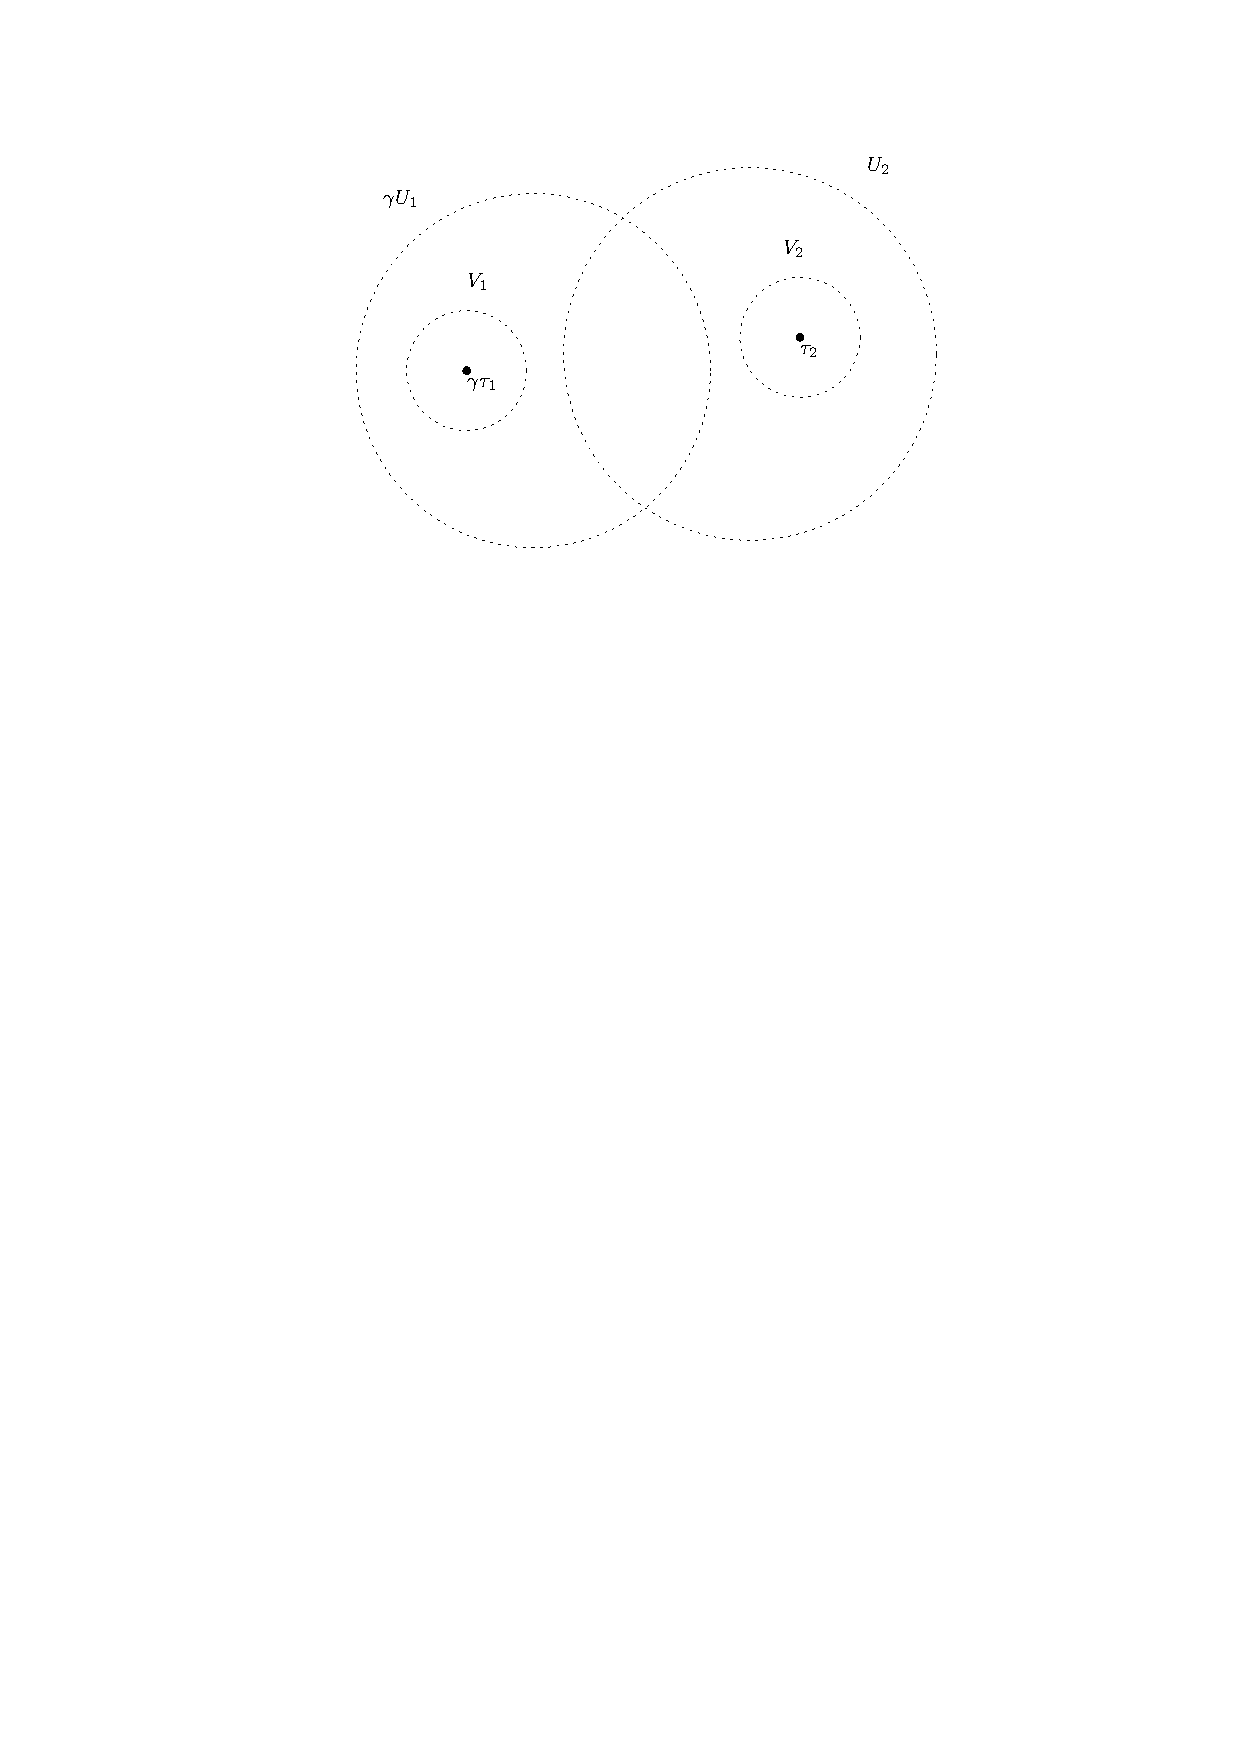
\includegraphics[height=3cm]{Pictures/shrinking-neighborhoods.pdf}
    \caption{Shrinking the neighborhoods}
    \label{fig:shriking-neighborhoods}
  \end{figure}
Since the set of $\gamma$ such that these intersections are nonempty is finite, this process terminates after a finite number of steps and will leave us with the right neighborhoods.
\end{proof}
\begin{corollary}
  The quotient $Y(1) = \SL_2(\ZZ)\backslash\HH$ is Hausdorff.
\end{corollary}
\begin{proof}
  Pick $\pi(\tau_1)\neq \pi(\tau_2)$ in $Y(1)$, and let $U_1$ and $U_2$ be neighborhoods as in the Proposition. For every $\gamma\in\SL_2(\ZZ)$ we have $\gamma\tau_1\neq \tau_2$ by the choice of $\tau_1$ and $\tau_2$. Therefore for every $\gamma\in\SL_2(\ZZ)$ we have $\gamma U_1\cap U_2=\emptyset$. Therefore $\pi(U_1)\cap\pi(U_2)=\emptyset$. It remains to show that $\pi(U_i)$ is an open set. Indeed, if $U\subseteq\HH$ is an open set, then
\[
\pi^{-1}(\pi(U)) = \cup_{\gamma\in\SL_2(\ZZ)} \gamma U
\]
is a union of open sets. Therefore it is open. We have showed that $\pi(U)$ is open (because of the quotient topology). Therefore each of the $\pi(U_i)$ is open, as we wanted to show.
\end{proof}

\section{Basic definitions of modular forms}
\label{sec:the-modular-group}

Let $\SL_2(\ZZ)\subset\SL_2(\RR)$ be the subgroup of matrices with entries in $\ZZ$ (and determinant $1$), which of course still acts on functions as we have seen.
\begin{definition}
  A holomorphic function $f\colon \HH\to\CC$ is called \emphh{weakly-modular} of weight $k\in\ZZ$ for $\SL_2(\ZZ)$ if $f|_k\gamma = f$ for all $\gamma\in\SL_2(\ZZ)$. Explicitly:
\begin{equation}
\label{eq:modular-transformation}
f(\gamma\cdot z) = j(\gamma,z)^k f(z),\quad\forall \gamma\in\SL_2(\ZZ).
\end{equation}

\end{definition}

Note that since $-I\in\SL_2(\ZZ)$, then there are no non-zero weakly-modular functions of odd weight:
\[
f(z)=(-1)^kf(z)\implies f=0.
\]

We will need an extra analytic property to define modular forms for $\SL_2(\ZZ)$. For now, note that:
\[
\frac{d(\gamma\cdot z)}{dz} = j(\gamma,z)^{-2},
\]
so we can rewrite the weakly-modular property by asking that the differential $f(z)(dz)^{k/2}$ is invariant under $\SL_2(\ZZ)$. It also shows that if~\eqref{eq:modular-transformation} holds for $\gamma_1$ and $\gamma_2$, then it also holds for $\gamma_1\gamma_2$.

We will see later (see Corollary~\ref{cor:STgenerate}) that $\SL_2(\ZZ)$ is generated by the matrices $T=\smtx 1101$ and $S=\smtx{0}{-1}{1}{0}$. Together with the previous observation, this implies that for $f$ to be weakly-modular it is enough to check~\eqref{eq:modular-transformation} for $T$ and $S$:
\[
f(z+1)=f(z),\quad f(-1/z) = z^k f(z).
\]

The transformation property (rather, the fact that $f(z+1)=f(z)$) implies that $f$ has a Fourier expansion. Another way to think about it is that there is a holomorphic map:
\[
\exp\colon \HH\to \{0<|q|<1\},\quad z\mapsto q=e^{2\pi i z}.
\]
If $f$ is holomorphic and $1$-periodic, then we can define $g(q)=f(z)$. That is, we may define:
\[
g(q)=f\left(\frac{\log q}{2\pi i}\right),
\]
where we may choose any branch of the logarithm because of the periodicity of $f$. The function $g$ is holomorphic on $D'$, and thus it has a Laurent expansion
\[
g(q)=\sum_{n=-\infty}^\infty a(n)q^n.
\]
Therefore $f$ has an expansion
\[
f(z) = \sum_{n=-\infty}^\infty a(n)e^{2\pi i nz}.
\]
\begin{definition}
  We say that $f$ is \emphh{meromorphic at infinity} (respectively \emphh{holomorphic at infinity}) if $f(z)=\sum_{n\geq n_0} a(n)q^n$ (respectively if in addition $n_0=0$).
\end{definition}
Note that checking that $f$ is holomorphic at infinity is the same as checking that $f(z)$ is bounded as $z$ approaches $i\infty$. If $f$ is holomorphic at infinity, then the value of $f$ at infinity is defined to be $f(\infty)=a(0)$.

\begin{definition}
  We say that $f$ \emphh{vanishes at infinity} if $n_0=1$. Equivalently, if $f(\infty)=0$.
\end{definition}

\begin{definition}
  Let $k\in \ZZ$ and let $f\colon\HH\to\CC$. We say that $f$ is a \emphh{modular form} of weight $k$ for $\SL_2(\ZZ)$ if:
  \begin{enumerate}
  \item $f$ is holomorphic,
  \item $f(\gamma z) = (cz+d)^kf(z)$ for all $\gamma=\smtx abcd\in\SL_2(\ZZ)$, and
  \item $f$ is holomorphic at infinity.
  \end{enumerate}
A \emphh{cusp form} is a modular form which vanishes at infinity.

The space of modular forms of weight $k$ is written $M_k=M_k(\SL_2(\ZZ))$, and it contains the space of cusp forms of weight $k$, which in turn is written $S_k=S_k(\SL_2(\ZZ))$.
\end{definition}


\begin{remark}
  If we replace ``holomorphic'' with ``meromorphic'' above, we obtain
  what can be called \emphh{meromorphic modular forms}. Other authors
  call them modular functions, but this name is used in different
  contexts and we will avoid it.
\end{remark}

Note that both  $M_k$ and $S_k$ are $\CC$-vector spaces. Also, multiplication of functions gives $M=\bigoplus_{k\in\ZZ} M_k$ the structure of a \emph{graded ring}. That is, $M_rM_s\subseteq M_{r+s}$. Finally,
for all odd $k$ one has $M_k = \{0\}$.


\section{Eisenstein series}
\label{sec:fourier-expansions-eisenstein}

For $k\geq 3$, define
\[
G_k(z) = \sumprime_{(m,n)\in \ZZ^2} (mz+n)^{-k}.
\]
\begin{lemma}
  $G_k$ converges absolutely for all $z$, and uniformly on sets of the form
\[
\Omega=\{z\in\HH~|~|\Re(z)|\leq A,\Im(z)\geq B\}.
\]
\end{lemma}
\begin{proof}[Sketch of proof]

First, show that
there exists a constant $C>0$ such that $|z+\delta|>C\sup\{1,|\delta|\}$ for all $z\in\Omega$ and $\delta\in\RR$.

Now, note that:
\begin{align*}
\sumprime |mz+n|^{-k} &= \sumprime |m|^{-k}|z+n/m|^{-k}<\sumprime C^{-k}|m|^{-k}\sup\{1,|n/m|\}^{-k}\\
&=C^{-k}\sumprime \sup\{|m|,|n|\}^{-k}.
\end{align*}
This last sum is easily seen to converge. For instance, one can sum over squares around the origin, of increasing size and compare to a $p$-series.

\end{proof}

The previous lemma ensures that $G_k(z)$ is a holomorphic function. Moreover, we have:
\begin{theorem}
  For each $k\geq 3$, $G_k$ is a modular form.
\end{theorem}

We will first show that $G_k$ is weakly modular.
\begin{proposition}
  For each $k\geq 3$ the holomorphic function $G_k$ is weakly modular.
\end{proposition}
\begin{proof}
Let $\gamma = \smtx abcd$ be a matrix in $\SL_2(\ZZ)$. We compute
\begin{align*}
G_k(\gamma z) &= \sumprime_{(m,n)} \left(m\frac{az+b}{cz+d} + n\right)^{-k}\\
&= \sumprime_{(m,n)} (cz+d)^k \left(m(az+b)+n(cz+d)\right)^{-k}\\
&= (cz+d)^k\sumprime_{(m,n)}\left( (am+cn)z + (bm+dn)\right)^{-k}.
\end{align*}
Note that the pair $(am+cn,bm+dn)$ is the result of multiplying the row vector $(m,n)$ by the matrix $\smtx abcd$. Since $\smtx abcd$ is invertible, the pair $(am+cn,bm+dn)$ runs through all values of $\ZZ^2$ as $(m,n)$ does. Therefore, by reordering the sum above we get:
\[
G_k(\gamma z) = (cz+d)^k \sumprime_{(m',n')} \left( m'z+n'\right)^{-k} = (cz+d)^k G_k(z),
\]
as wanted.
\end{proof}
It remains to show that $G_k$ is holomorphic at infinity. In fact, we will compute its Fourier series. We start by introducing the \emphh{Bernoulli numbers}, which appear in the Fourier series for $G_k$.

\begin{definition}
  The \emphh{Bernoulli numbers} are defined\footnote{These are called ``first Bernoulli numbers'', and differ by a sign from those defined originally by Bernoulli.} by:
\begin{equation}
\label{eq:bernoulli-numbers}
\frac{x}{e^x -1} = \sum_{k=0}^\infty B_k \frac{x^k}{k!} = 1 -\frac 1 2 x + \frac 1{6} \frac{x^2}{2} - \frac 1{30}\frac{x^4}{24} + \cdots.
\end{equation}
\end{definition}
Recall the definition of Riemann's zeta function
\[
\zeta(s) = \sum_{n=1}^\infty \frac{1}{n^s},\quad \Re(s)>1.
\]
It has a simple pole of residue $1$ at $s=1$, and extends to a meromorphic function on $\CC$, holomorphic on $\CC\setminus \{1\}$. The Bernoulli numbers appear also naturally in the formulas:
\begin{equation}
\label{eq:bernoulli-zeta}
\zeta(k) = \sum_{n=1}^\infty \frac{1}{n^k} = -\frac{(2\pi i)^k}{2}\frac{B_k}{k!},\quad \forall k \geq 2,\quad \zeta(1-n) = -\frac{B_n}{n},\quad \forall n \geq 1.
\end{equation}
An odd prime $p$ is called \emphh{regular} if $p$ does not divide the numerator of $B_2$, $B_4$,\ldots $B_{p-3}$. This is equivalent to $p$ not dividing the class number of $\QQ(\sqrt[p]{1})$. Under this assumption, Fermat's Last Theorem was proved by Kummer around 1850, and probably by Fermat himself. Although Siegel conjectured that about $60\%$ of primes are regular, it is not know even whether there are infinitely many of them.

We will derive the Fourier expansion of $G_k$ from that of the cotangent:
\begin{lemma}
\label{lemma:cotangent}
  The following identity of holomorphic functions holds.
\[
\frac 1z + \sum_{d=1}^\infty\left(\frac 1{z-d} + \frac 1{z+d}\right) = \pi\cot(\pi z) = \pi i - 2\pi i\sum_{m=0}^\infty q^m,\quad q = e^{2\pi i z}.
\]
\end{lemma}
\begin{proof}
  Consider Euler's product formula for the sine function:
\[
\sin(\pi z) = \pi z \prod_{n=1}^\infty \left(1-\frac{z^2}{n^2}\right).
\]
Taking the logarithmic derivative of this equation yields
\[
\pi\cot(\pi z) = \frac 1 z + \sum_{d=1}^\infty \frac{2z}{z^2-n^2} = \frac 1z + \sum_{d=1}^\infty \left(\frac 1{z-d}+\frac 1{z+d}\right).
\]
On the other hand, we can use the expression of $\sin$ and $\cos$ in terms of the exponential function to write:
\begin{align*}
\pi\cot(\pi z)&=\pi \frac{\cos(\pi z)}{\sin(\pi z)} = \pi \frac{\frac{e^{i\pi z} + e^{-i\pi z}}{2}}{\frac{e^{i\pi z} - e^{-i\pi z}}{2i}}=\pi i\frac{e^{i\pi z} + e^{-i\pi z}}{e^{i\pi z} - e^{-i\pi z}}\\
&=\pi i\left(1 - 2\frac{e^{-i\pi z}}{e^{-i\pi z} - e^{i\pi z}}\right)=\pi i\left(1 - 2\frac{1}{1 - e^{2\pi i z}}\right).
\end{align*}
Finally, write $q=e^{2\pi i z}$ and the formula follows from the identity
\[
\frac{1}{1-q} = \sum_{m=0}^\infty q^m,\quad |q|<1.
\]
\end{proof}
\begin{lemma}
\label{lemma:expansion-latticesum}
For each $k\geq 2$ we have
\[
\sum_{d\in\ZZ}\frac{1}{(z+d)^k} = \frac{(-2\pi i)^k}{(k-1)!}\sum_{n=1}^\infty n^{k-1}q^n.
\]
\end{lemma}
\begin{proof}
From Lemma~\ref{lemma:cotangent} we have
\begin{equation}
\frac 1z + \sum_{d=1}^\infty\left(\frac 1{z-d} + \frac 1{z+d}\right) = \pi i - 2\pi i\sum_{d=0}^\infty q^d,\quad q = e^{2\pi i z}.
\end{equation}
Differentiating both sides with respect to $z$ gives
\[
\frac{-1}{z^2}+\sum_{d=1}^\infty \left(\frac{-1}{(z-d)^2}+\frac{-1}{(z+d)^2}\right) = -(2\pi i)^2 \sum_{d=1}^\infty dq^d.
\]
Since each of the terms in the infinite sum of the left hand side converges absolutely, we can reorder the series and obtain the identity
\[
\sum_{d\in \ZZ} \frac{1}{(z+d)^2} = (2\pi i)^2\sum_{d=1}^\infty dq^d.
\]
This is proves the formula for $k=2$. The identity for general $k$ follows by induction, by differentiating the identity for $k-1$.
\end{proof}
We have finally all the ingredients to prove the sought expansion. As a piece of notation for the next result, for $m\geq 0$ the \emphh{$m$-divisor function} is:
\[
\sigma_{m}(n)=\sum_{d\mid n} d^{m}.
\]
\begin{theorem}
  Let $k\geq 4$ be even. Then
\[
G_k(z) = 2\zeta(k) E_k(z), \text{ where } E_k(z) = 1-\frac{2k}{B_k}\sum_{n=1}^\infty \sigma_{k-1}(n)q^n\in\QQ\bbl q\bbr.
\]
\end{theorem}
\begin{proof}
  Consider now $k\geq 4$ and calculate
\begin{align*}
G_k(z)=\sumprime_{(m,n)\in\ZZ^2} \frac{1}{(mz+n)^k} &= \sum_{n\neq 0} \frac{1}{n^k} + \sum_{m\neq 0}\sum_{n\in\ZZ} \frac{1}{(mz+n)^k}\\
&=2\zeta(k) + 2\sum_{m=1}^\infty \sum_{n\in\ZZ}\frac{1}{(mz+n)^k}.
\end{align*}
Here we have used the definition of Riemann's zeta function at $k$ and the fact that $k$ is even. Using now the formula of Lemma~\ref{lemma:expansion-latticesum} where $z$ gets substituted by $mz$, we can replace the second term, and obtain the formula
\begin{align*}
G_k(z) &= 2\zeta(k)+2\sum_{m=1}^\infty\left( \frac{(-2\pi i)^k}{(k-1)!}\sum_{d=1}^\infty d^{k-1} q^{dm}\right) = 2\zeta(k) + \frac{2\cdot (-2\pi i)^k}{(k-1)!} \sum_{m=1}^\infty\sum_{d=1}^\infty d^{k-1}q^{md}.
\end{align*}
Finally, group the terms in the inner sum that contribute to $q^n$. These consist of all pairs of positive integers $(m,d)$ such that $md=n$. That is, for each $n$ we must consider all divisors $d'$ of $n$, and we can rewrite:
\[
\sum_{m=1}^\infty\sum_{d=1}^\infty d^{k-1} q^{md} = \sum_{n=1}^\infty \sigma_{k-1}(n)q^n.
\]
This gives the desired expansion, by using the formula of Equation~\eqref{eq:bernoulli-zeta}.
\end{proof}
\begin{example}
Define the \emphh{Eisenstein series}
\[
E_4 = 1 + 240\sum_{n=1}^\infty \sigma_3(n)q^n\in M_4
\]
and
\[
E_6 = 1 - 504\sum_{n=1}^\infty \sigma_5(n)q^n\in M_6.
\]
Since both $E_4^3$ and $E_6^2$ are both in $M_{12}$, its difference is also there. Computing we see that
\[
E_4^3-E_6^2 = (1+720q+\cdots)-(1-1008q+\cdots) = 1728q+\cdots\in S_{12},
\]
and thus we may define
\[
\Delta(z)=\frac{E_4^3-E_6^2}{1728} = q-24q^2+252q^3+\cdots,
\]
which is a cusp form of weight $12$.
\end{example}

\section{Fundamental domains}
\begin{figure}[h]
\centering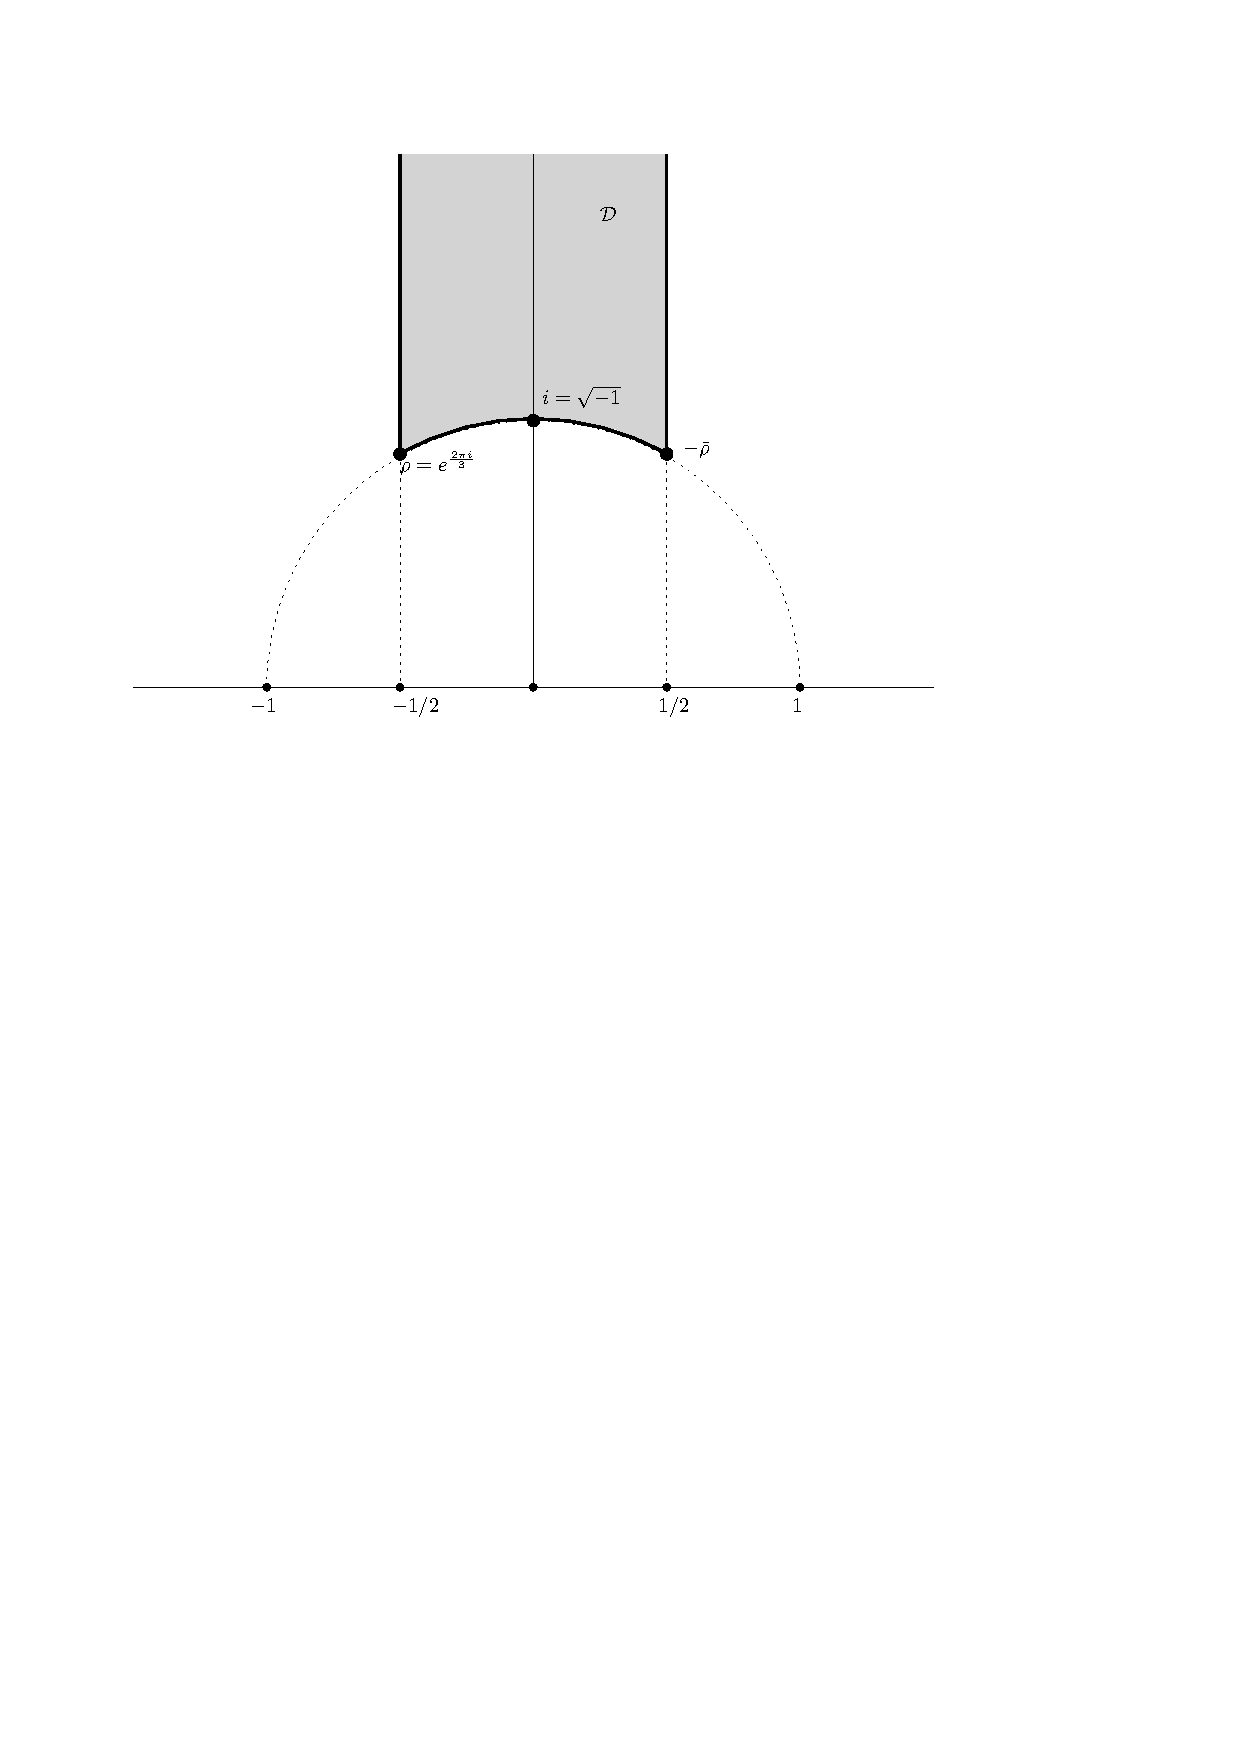
\includegraphics[scale=0.5]{fundomSL2Z.pdf}
\caption{Fundamental domain for $\SL_2(\ZZ)$}
\end{figure}

\begin{definition}
  Let $\Gamma$ be a group acting on $\HH$. A \emphh{fundamental domain} for $\Gamma$ is closed subset $\cD\subset\HH$ such that
  \begin{enumerate}
  \item The set $\cD$ is the closure of its interior.
  \item Every point in $\HH$ is $\Gamma$-equivalent to a point of $\cD$.
  \item If $z,z'\in\cD$ are two distinct points which are $\Gamma$-equivalent then they lie on the boundary of $\cD$.
  \end{enumerate}
\end{definition}

\begin{theorem}
  The subset $\cD$ of $\HH$ as above is a (connected) fundamental domain for $\SL_2(\ZZ)$.

Moreover the stabilizer $H_z$ of a point $z\in\cD$ in $\SL_2(\ZZ)$ is
\[
H_z=\begin{cases}
C_6=\langle ST\rangle = \langle\smtx{0}{-1}{1}{1}\rangle  & z = \rho,\\
C_6'=\langle TS\rangle =\langle \smtx{1}{-1}{1}{0}\rangle & z=\rho + 1,\\
C_4=\langle S\rangle =\langle \smtx{0}{-1}{1}{0}\rangle & z=i,\\
C_2=\langle -I\rangle =\langle \smtx{-1}{0}{0}{-1}\rangle&\text{ else.}
\end{cases}
\]
\end{theorem}
\begin{proof}
  Let $z\in \HH$. We have seen that, if $\gamma\in\SL_2(\ZZ)$, then
\[
\Im(\gamma z) = \frac{\Im(z)}{|cz+d|^2},\quad \gamma = \mtx abcd.
\]
There are finitely many pairs $(c,d)\in\ZZ^2$ such that $|cz+d|<1$. In particular,
one can choose a matrix $\gamma\in\langle S,T\rangle\subseteq \SL_2(\ZZ)$ such that
\[
\Im(\gamma z)\geq \Im(\gamma' z),\quad \forall \gamma'\in \langle S,T\rangle\subseteq\SL_2(\ZZ).
\]
By premultiplying $\gamma$ by an appropriate power of $T$ (which does not change the imaginary part), we may and do assume that $|\Re(\gamma z)|\leq \frac 12$. We will now show that $|\gamma z|\geq 1$:
\[
\Im(\gamma z)\geq \Im(S\gamma z)=\Im(-1/\gamma z)=\frac{\Im(\gamma z)}{|\gamma z|^2}.
\]
This implies $|\gamma z|\geq 1$, and hence $\gamma z\in \cD$, thus proving $(1)$.

In order to show $(2)$, suppose that $z'=\gamma z$ and both $z$ and $z'$ lie in $\cD$. Without loss of
generality, we may assume that $\Im(\gamma z)\geq \Im(z)$, or equivalently that
\[
|cz+d|^2=|cx+d|^2+|cy|^2\leq 1.\quad\text{ (we write $z=x+iy$).}
\]
Since $y>1/2$, this implies that $|c|\leq 1$. The case $c=0$ gives that $|d|\leq 1$ and since $\smtx abcd\in\SL_2(\ZZ)$ this means that $\gamma=\pm\smtx 1 b01$, a translation matrix. Therefore $z'=z\pm 1$.

Let us suppose that $c=1$ (the case $c=-1$ is completely analogous). Then the condition $|z+d|^2\leq 1$ is only satisfied when $|z|=1$ ($d=0$), when $z=\rho$ ($d=1$), or when $z=\rho+1$ ($d=-1$), giving $(2)$.

To study the stabilizers of points $z\in\cD$, we can use the calculations that we have used to show $(2)$. If $\gamma z = z$, then necessarily $c=\pm 1$, and by changing $\gamma$ to $-\gamma$ we may assume $c=1$. The quadratic equation given by $\gamma z = z$ gives that $|a+d|<2$, so $|a+d|\leq 1$. At the same time, the fact that $z\in\cD$ gives $|a-d|\leq 1$. Together, these two inequalities give $|a|\leq 1$. We obtain the following possibilities:
\begin{table}[h]
\begin{tabular}{cccc}
\toprule
$\gamma$&$z$&$z'=\gamma z$&fixed points\\
\midrule
$\pm \smtx 1001$&all&$z$&all\\[5pt]
$\pm \smtx 1101$&$\Re(z)=-\frac 12$&$z+1$&none\\[5pt]
$\pm \smtx 1{-1}01$&$\Re(z)=\frac 12$&$z-1$&none\\[5pt]
$\pm \smtx 0{-1}10$&$|z|=1$&$-1/z$&$i$\\[5pt]
$\pm \smtx {-1}{-1}{1}{0},\pm \smtx{0}{-1}{1}{1}$&$\rho$&$\rho$&$\rho$\\[5pt]
$\pm \smtx {1}{-1}{1}{0},\pm \smtx{0}{-1}{1}{-1}$&$\rho+1$&$\rho+1$&$\rho+1$
\end{tabular}
\end{table}
By studying this table we conclude the classification of stabilizers.
\end{proof}
\begin{corollary}
\label{cor:STgenerate}
  The group $\SL_2(\ZZ)$ is generated by the matrices $T$ and $S$.
\end{corollary}
\begin{proof}
  Let $z_0$ be a point in the interior of $\cD$. Given $\gamma\in\SL_2(\ZZ)$, the theorem provides a matrix $\delta\in\langle T,S\rangle$ such that $\delta\gamma^{-1} z_0\in\cD$. Therefore $\delta\gamma^{-1} z_0 = z_0$ and hence $\delta\gamma^{-1} = \pm I$. Since $S^2=-I$, we are done by possibly multiplying $\delta$ by $S^2$.
\end{proof}

\section{Valence formula}
\label{sec:valence-formula}

Let $f$ be a meromorphic function on some open subset of $\HH$. Write $v_p(f)$ for the order (or valuation) of $f$ at $p\in \HH\cup\{\infty\}$. This is the unique integer
$n$ such that $(z-p)^{-n}f(z)$ is holomorphic and non-vanishing at $p$. If $n$ is positive we
say that $f$ has a zero of order $n$, and if $n$ is negative we say that $f$ has a pole of order $-n$. If $f$ is weakly modular and meromorphic at infinity, then also define $v_\infty(f)=n_0$ if
\[
f(q)=\sum_{n\geq n_0} a_n q^n,\quad a_{n_0}\neq 0.
\]
Next, suppose that $f$ has a Laurent expansion of the form
\[
f(z) = \sum_{n\geq n_0} c_n (z-p)^n.
\]
The \emphh{residue} of $f$ at $p$ is $\res_p(f) = c_{-1}\in\CC$. One can calculate
the order of $f$ at $p$ by using residues, using the following lemma.
\begin{lemma} If $f$ is a meromorphic function around a point $p$, then
  \[
\res_p(f'/f) = v_p(f).
\]
\end{lemma}
\begin{proof}
If $v_p(f)=n$, write $f(z)=(z-p)^ng(z)$ with $g(z)$ holomorphic and non-vanishing at $p$. Then calculate the residue of $f'/f$ by hand.
\end{proof}
We recall without proof two basic results of complex analysis.
\begin{theorem}[Cauchy's integral formula]
  Let $g$ be a holomorphic function on an open subset $U\subseteq\CC$ and let $C$ be a contour in $U$. For each $p\in U$,
\[
\int_C \frac{g(z)}{z-p}dz = 2\pi i g(p).
\]
\end{theorem}
\begin{corollary}
  Let $C(p,r,\alpha)$ be an arc of a circle, of radius $r$ and angle $\alpha$ around a point $p$. If $g$ is holomorphic at $p$, then
\[
\lim_{r\to 0}\int_{C(p,r,\alpha)} \frac{g(z)}{z-p}dz = \alpha i g(p).
\]
\end{corollary}
The following result relates the contour integral of the logarithmic derivative of $f$ to the orders of $f$ at the interior points.
\begin{theorem}[argument principle]
  Let $f$ be a meromorphic function on an open subset $U\subseteq \CC$ and let $C$ be a contour in $U$ not passing through any zeros or poles of $f$. Then:
\[
\int_C\frac{f'(z)}{f(z)}dz = 2\pi i \sum_{z\in\operatorname{int}(C)} v_z(f).
\]
\end{theorem}

\begin{corollary}
  Let $C(p,r,\alpha)$ be an arc of a circle, of radius $r$ and angle $\alpha$ around a point $p$. If $f$ is meromorphic at $p$, then
\[
\lim_{r\to 0}\int_{C(p,r,\alpha)} \frac{f'(z)}{f(z)}dz = \alpha i v_p(f).
\]
\end{corollary}
We will study weakly modular meromorphic functions $f\colon \HH\to \CC$. In this case, the order of vanishing makes sense in $\SL_2(\ZZ)$-orbits: suppose that $f$ has weight $k$. Then an easy computation shows that, for $\gamma\in\SL_2(\ZZ)$,
\[
\lim_{z\to\gamma p} (z-\gamma p)^{-n}f(z) = j(\gamma,p)^{k+2n}\lim_{z\to p} (z-p)^{-n}f(z).
\]
But note now that $j(\gamma,p)$ is nonzero because $p\not\in \QQ\cup\{\infty\}$. We conclude that $v_p(f)=v_{\gamma p}(f)$.

\begin{theorem}[valence formula]
\label{thm:valence-formula}
  Let $f$ be a non-zero weakly modular meromorphic form of weight $k$ on $\SL_2(\ZZ)$. Then:
\[
v_\infty(f)+\frac 12 v_i(f)+\frac 13 v_\rho(f) + \sum_{\tau\in \SL_2(\ZZ)\backslash\HH'} v_\tau(f) = \frac{k}{12}.
\]
Here the sum runs through the orbits in $\SL_2(\ZZ)\backslash\HH$ other than those of $i$ and $\rho$.
\end{theorem}

Before proving this theorem we will see how helpful it is in studying the spaces of modular forms.
\begin{theorem}
  \begin{enumerate}
  \item $M_k=\{0\}$ if $k<0$ or $k = 2$.
  \item $S_k=\{0\}$ if $k < 12$.
  \item $M_0=\CC$.
  \item $S_{12} = \CC\Delta$.
  \end{enumerate}
\end{theorem}
\begin{proof}
  \begin{enumerate}
  \item   Since the left-hand side of the valence formula is non-negative, the right hand side must be non-negative too, hence $k\geq 0$. If $k=2$, then we get $1/6$ on the right-hand side. However, the left-hand side is a sum of non-negative multiples of $1$, $1/2$ and $1/3$, thus a contradiction.
\item   If $0\neq f\in S_k$, then $v_\infty(f)\geq 1$. Therefore the valence formula gives $k\geq 12$.
\item Let $f\in M_0$. Since the constant function $g=f(\infty)$ also belongs to $M_0$, the difference $f-g$ belongs to $S_0=\{0\}$. Therefore $f=g$ is constant, and $M_0=\CC$ is the space of constant functions on $\HH$.
\item  If $f\in S_{12}$, then $v_\infty(f)\geq 1$. Therefore by the valence formula $v_\infty(f)=1$ and $f$ has no other zeros or poles. Define
\[
g(z)=f(z)-\frac{f(i)}{\Delta(i)}\Delta(z).
\]
Then $g(z)\in S_{12}$ and $g(i)=0$. If $g$ is non-zero, then the valence formula applied to $g$ would give a contradiction because $v_\infty(g)\geq 1$ and $v_i(g)\geq 1$. Therefore $g=0$ and $f$ is a multiple of $\Delta$.
  \end{enumerate}
\end{proof}

\begin{corollary}
\begin{enumerate}
  \item For all $k$, we have $S_{k+12} = \Delta M_{k}$.
\item For $k\geq 4$ we have
\[
M_k = (\CC E_k) \oplus S_k
\]
\item 
If $k$ is odd or negative then $M_k = \{0\}$. For each even $k\geq 2$, we have:
\[
\dim(M_k)=\begin{cases}
\lfloor\frac k{12}\rfloor & k\equiv 2\pmod{12},\\
1+ \lfloor\frac k{12}\rfloor & k\not\equiv 2\pmod{12}.
\end{cases}
\]
\end{enumerate}
\end{corollary}

\begin{proof}
For $k<0$ the first statement is trivial, and we just proved it also for  $k=0$. Given $f\in S_{k+12}$, the function $g=f/\Delta$ is holomorphic on $\HH$ because $\Delta$ is non-vanishing, and it belongs to $M_k$ because $v_\infty(g)=v_\infty(f)-v_\infty(\Delta)=v_\infty(f)-1\geq 0$.

Consider the linear map
\[
\varphi\colon M_k\to\CC,\quad f\mapsto f(\infty).
\]
Then $S_k=\ker\varphi$. Also $\varphi$ is surjective because $\varphi(E_k)=1$. Therefore $M_k=\CC E_k\oplus S_k$.

Note that this gives a recursive way to obtain $M_k$:
\[
M_k = \CC E_k \oplus S_k = \CC E_k \oplus (\Delta M_{k-12}).
\]

For $k$ odd we know that $M_k=\{0\}$ by the weak-modularity condition. For $k<0$ we also know $M_k=\{0\}$ by the previous part. We prove the remaining formula by induction on $k$. Note that we already know it for $k=0$ and $k=2$. For $k=4, 6, 8, 10$ then since $\dim(M_k)=1+\dim(S_k)=1+\dim(M_{k-12}) = 1$ we get $\dim(M_k)=1$. If $k$ is even and $k\geq 12$, then:
\[
\dim(M_k)=1+\dim(M_{k-12}).
\]
\end{proof}
\begin{corollary}
  The space $M_k$ has for basis the following set:
\[
M_k=\langle E_4^aE_6^b~|~ a\geq 0,b\geq 0, 4a+6b=k\rangle.
\]
\end{corollary}
\begin{proof}
  We start by showing that the given monomials $E_4^aE_6^b$ generate $M_k$. For $k=2,4,6$ this is clear because we know $M_2=\{0\}$, and $M_4=\CC E_4$ and $M_6=\CC E_6$. For $k\geq 8$ we induct on $k$. Choose some
 pair $(a,b)$ such that $4a+6b=k$ (convince yourself that this is always possible). If $f\in M_k$, then since $E_4^aE_6^b (\infty)=1$, the function $g(z)=f(z)-f(\infty)E_4^aE_6^b$ is a cusp form in $S_k$. Therefore $g=\Delta h$, for
some $h\in M_{k-12}$. By induction hypothesis, $h$ is a linear combination of monomials $E_4^xE_6^y$ for appropriate pairs $(x,y)$. Using the expression $\Delta=\frac{1}{1728}(E_4^3-E_6^2)$ we deduce the result for $f$.

Now we show that the given monomials are linearly independent. We can use induction on $k$ in steps of $12$ once more, to show that the number of such monomials agrees with $\dim M_k$. This can be checked by hand for $k\leq 14$. Suppose that $k\geq 14$. Note that each monomial $E_4^aE_6^b$ of weight $k-12$ gives a monomial $E_4^aE_6^{b+2}$ of weight $k$. All such monomials are obtained in this way, except for those of the form $E_4^a$ or $E_4^aE_6$. When $k\equiv 0\pmod 4$ then $E_4^{k/4}$ is of weight $k$, and when $k\equiv 2\pmod 4$ then $E_4^{(k-6)/2}E_6$ is of weight $k$, thus in any case there is exactly one more monomial of weight $k$ than there are of weight $k-12$. This completes the proof.
\end{proof}

\begin{example}
  This allows to write down all spaces of modular and cusp forms for $\SL_2(\ZZ)$. For example,
\[
M_{18} = \CC E_{18}\oplus S_{18} = \CC E_{18} \oplus \Delta M_6 = \CC E_{18}\oplus \CC\Delta E_6.
\]
\[
M_{30} = \CC E_{30} \oplus \CC\Delta E_{18} \oplus \CC \Delta^2 E_6.
\]
Another basis for the same space (which is better because it is expressed in terms of $E_4$, $E_6$ and $\Delta$):
\[
M_{30} = \CC E_6^5\oplus \Delta E_6^3 \oplus \Delta^2 E_6.
\]
Note that these forms are linearly independent (why?). Since $\dim M_{30}=3$, they form a basis.
\end{example}

\begin{remark}
  Suppose that $f(z)$ is a non-zero weakly-modular form of weight $0$. Then $f(\gamma z)=f(z)$. By the valence formula, $f$ has the same number of zeros as poles. This number is called the \emphh{valence} of $f$, and hence the name for the theorem.
\end{remark}

Another very powerful application of the valence formula is the following:
\begin{theorem}
  Let $f$ be a modular form of weight $k$. Suppose that $f$ has a $q$-expansion of the form $\sum_{n\geq 0} a_nq^n$. If $a_j=0$ for all $0\leq j\leq k/12$, then $f=0$.
\end{theorem}
\begin{proof}
  The hypothesis means that $v_\infty(f) > k/12$. This is incompatible with the valence formula, and thus $f$ must be zero.
\end{proof}
\begin{corollary}
  Let $f$ and $g$ be two modular forms of the same weight $k$, and suppose that their $q$-expansions coincide for the first $\lfloor k/12\rfloor$ coefficients. Then $f=g$.
\end{corollary}

\subsection{The modular invariant \texorpdfstring{$j$}{j}}
  Define the function
\[
j(z)=\frac{E_4^3}{\Delta} = \frac{1+\cdots}{q+\cdots} = q^{-1} + 744 + 196884 q + \cdots.
\]
\begin{proposition}
  \begin{enumerate}
  \item $j$ is a meromorphic weakly-modular form of weight $0$.
  \item $j$ is holomorphic on $\HH$ and has a simple pole at infinity.
  \item It induces a bijection $\SL_2(\ZZ)\backslash\HH\to \CC$.
  \end{enumerate}
\end{proposition}
\begin{proof}
The fact that $j$ it is meromorphic weakly-modular of weight $0$ follows from it being a quotient of two modular forms of weight $12$.

Since $E_4$ is non-vanishing at infinity and $\Delta$ has a simple zero then $j=E_4^3/\Delta$ has a simple pole at infinity (we can also see it from its $q$-expansion, which starts with $q^{-1}$). The valence formula shows that $v_\rho(E_4)=1$, and therefore $j(z)$ has a triple zero at $\rho$. It is holomorphic on $\HH$ because $\Delta$ is non-vanishing on $\HH$.

Fix $c\in\CC$. The function $j(z)-c=q^{-1}+744-c+\cdots$ is another meromorphic weakly-modular function of weight $0$ and has a simple pole at $\infty$. The valence formula gives in this case that $j(z)-c$ has exactly one zero on $\SL_2(\ZZ)\backslash\HH$. This gives the last claim.
\end{proof}

\subsection{Proof of the valence formula}
The proof presented here avoids algebraic geometry, at the cost of some complex analysis. Let
$f$ be a modular function, and consider the following contour:
\begin{figure}[h]
  \centering
  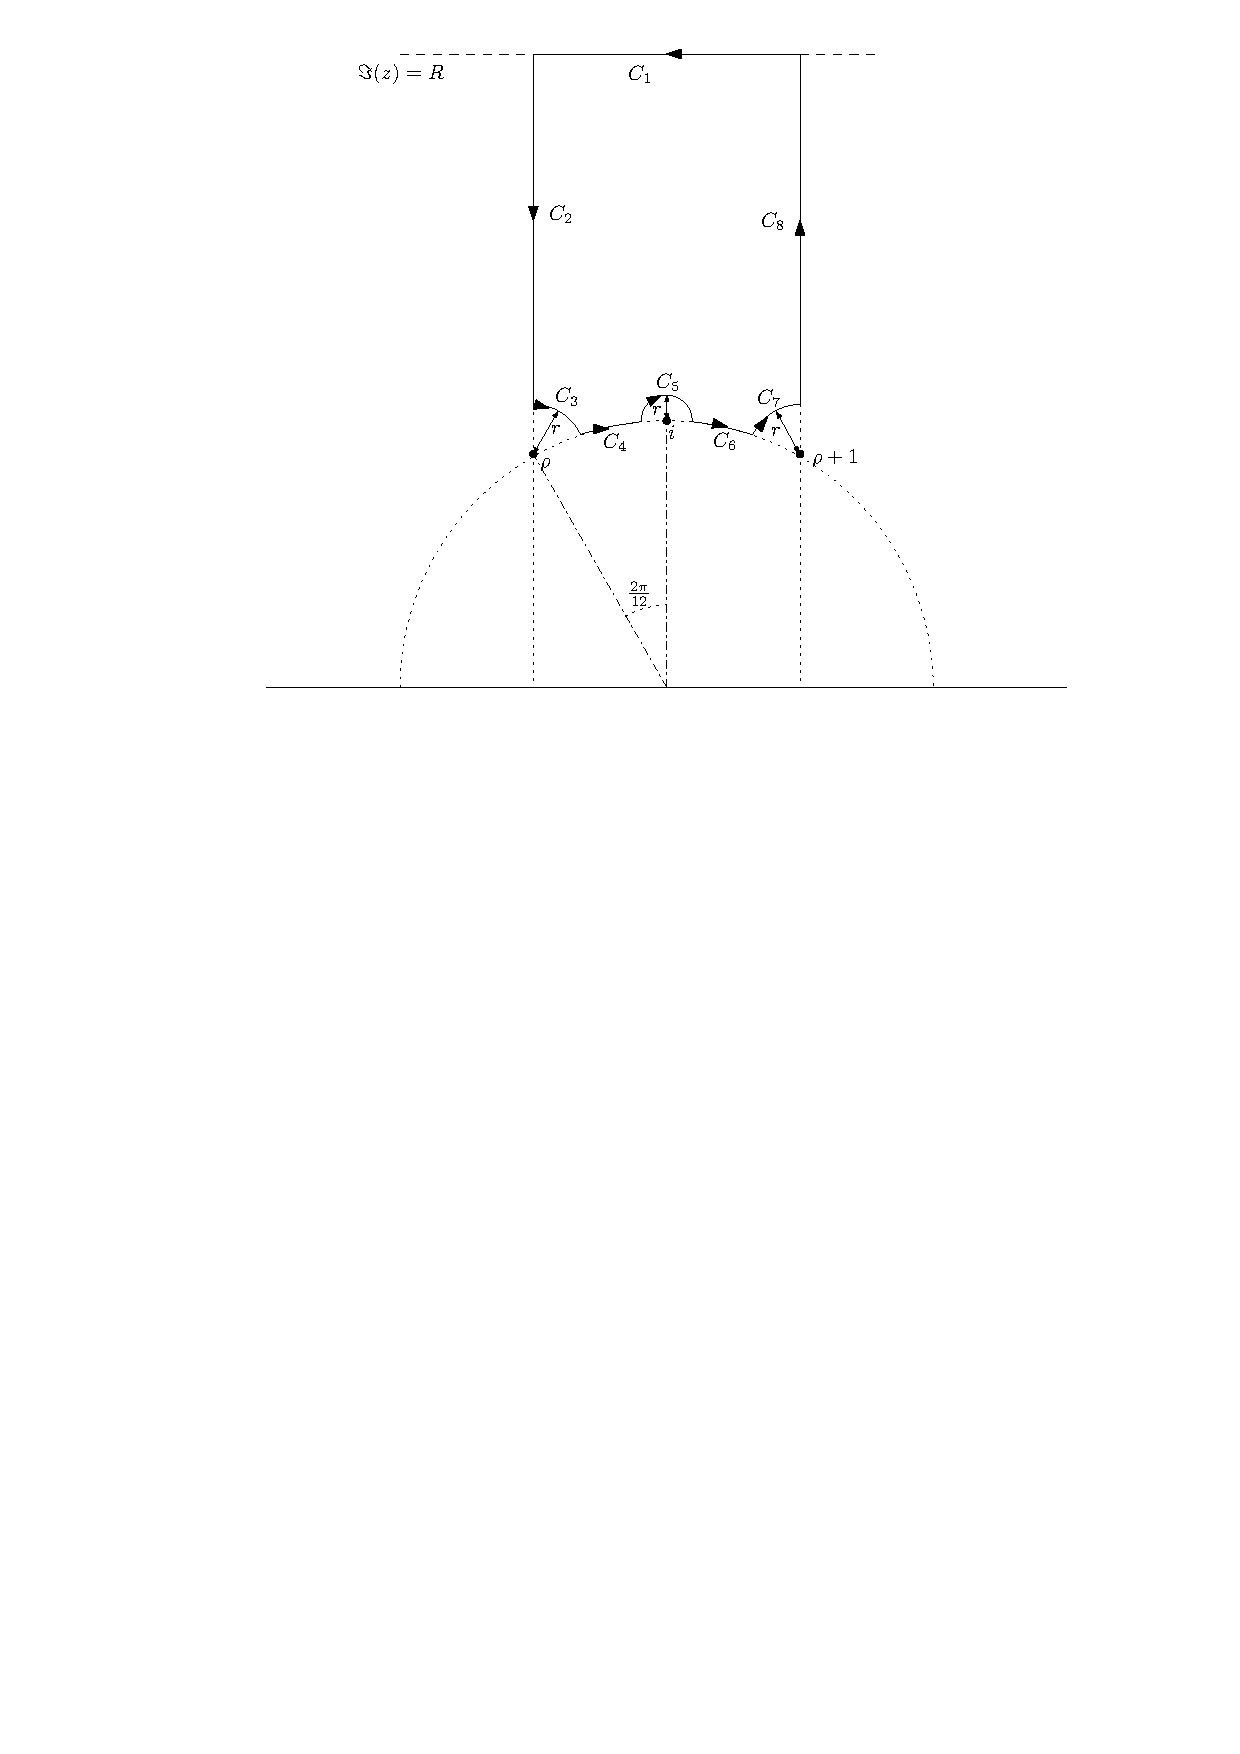
\includegraphics[height=6cm]{contour.pdf}
  \caption{Contour to integrate}
  \label{fig:contour}
\end{figure}

The proof consists in integrating $f'(z)/f(z)$ around the indicated contour $C$ in two different ways.
\paragraph{Integral residue formula:} This is the first way in which we calculate the contour integral. For $R$ large enough so that the contour contains all zeros and poles of $\SL_2(\ZZ)\backslash\HH'$ with large imaginary part, we have:
\[
\int_C \frac{f'(z)}{f(z)}dz = 2\pi i \sum_{p\in\operatorname{int}(C)} \res_p\left(\frac{f'}{f}\right) = 2\pi i\sum_{p\in \SL_2(\ZZ)\backslash\HH'} v_p(f).
\]
The rest of the proof consists in computing the integral as the sum of the path integrals along $C_1$,\ldots, $C_8$.
\paragraph{Integral along $C_1$:} Perform the change of variables $q(z)=e^{2\pi i z}$. Note that:
\[
dq = 2\pi i qdz,\quad dz = \frac{1}{2\pi i}\frac{dq}{q}.
\]
Moreover, the path $q(C_1)$ is a clockwise circle of radius $e^{-2\pi R}$ centered around $0$. Finally,
\[
\frac{d}{dz}f(q) = \frac{d}{dz} f(e^{2\pi i z}) = 2\pi i q f'(q).
\]
Putting these together, we obtain:
\[
\int_{C_1}\frac{f'(z)}{f(z)}dz = \int_{q(C_1)} \frac{f'(q)}{f(q)} dq.
\]
Since $f$ is meromorphic around infinity, this last quantity equals $- v_\infty(f)$.

\paragraph{Integral along $C_2$ and $C_8$:} Note that since $f$ is modular it satisfies $f(z+1)=f(z)$. Therefore also $f'(z+1)=f'(z)$, and we get, by changing $w=z+1$:
\begin{align*}
\int_{C_8}\frac{f'(w)}{f(w)}dw &= -\int_{C_2}\frac{f'(z+1)}{f(z+1)}dz = -\int_{C_2}\frac{f'(z)}{f(z)}dz.
\end{align*}
Therefore the contributions of $C_2$ and $C_8$ cancel out.

\paragraph{Integral along $C_4$ and $C_6$:} In the same way that for $C_2$ and $C_8$ we considered the change $z\mapsto z+1$, here we consider the change $z\mapsto s(z)=-z^{-1}$. This change of variables transforms $C_4$ to $-C_6$. Weak-modularity of $f$ implies also that $f(z) = z^{-k}f(s(z))$. Differentiating both sides yields:
\[
f'(z) = -kz^{-k-1}f(s(z)) + z^{-k}f'(s(z))s'(z).%\implies z^{-k}f'(-z^{-1})z^{-2} = -f'(z) - kz^{-k-1}f(-z^{-1}).
\]
This gives
\[
\frac{f'(z)}{f(z)} = \frac{-k}{z} + \frac{f'(s(z))s'(z)}{f(s(z))}.
\]
Therefore we may compute
\begin{align*}
\int_{C_4}\frac{f'(z)}{f(z)}dz &=\int_{C_4} \frac{-k}{z}dz + \int_{C_4}\frac{f'(s(z))s'(z)}{f(s(z))}dz =2\pi i\frac{k}{12} +\int_{-C_6}\frac{f'(s)}{f(s)}ds,
\end{align*}
and hence
\[
\int_{C_4+C_6}\frac{f'(z)}{f(z)}dz \to_{r\to 0} 2\pi i\frac{k}{12}.
\]

\paragraph{Integral along $C_5$:} Using the argument principle we obtain
\[
\int_{C_5} \frac{f'(z)}{f(z)}dz \stackrel[r\to 0]{}\longrightarrow -\frac 12 2\pi i v_i(f).
\]

\paragraph{Integrals along $C_3$ and $C_7$:} Applying again the argument principle we obtain
\[
\int_{C_3} \frac{f'(z)}{f(z)}dz \stackrel[r\to 0]{}\longrightarrow -\frac 16 2\pi i v_\rho(f),\text{ and}\quad
\int_{C_5} \frac{f'(z)}{f(z)}dz \stackrel[r\to 0]{}\longrightarrow -\frac 16 2\pi i v_{\rho+1}(f)=-\frac{1}{6}2\pi i v_\rho(f).
\]
Therefore
\[
\int_{C_3+C_5} \frac{f'(z)}{f(z)}dz \stackrel[r\to 0]{}\longrightarrow -\frac{1}{3}2\pi i v_\rho(f).
\]

\paragraph{Conclusion:} Putting together all the above calculations yields the sought formula.\qed

\section{A product formula for \texorpdfstring{$\Delta(z)$}{Delta(z)}}
\label{sec:a-product-formula-for-Delta}

Consider the weight-$2$ Eisenstein series
\[
G_2(z)=\sum_c\sumprime_d \frac{1}{(cz+d)^2},
\]
which does not converge absolutely. It is \emph{not} a weight-$2$ modular form (there are no such other than $0$), but we still have the formula:
\[
G_2(z)=2\zeta(2)E_2(z),\quad E_2(z)=1-24\sum_{n=1}^\infty \sigma_1(n)q^n.
\]
The function $E_2(z)$ is holomorphic on $\HH$, and $E_2(z+1)=E_2(z)$. However, we are about to see that
\[
z^{-2}E_2(-1/z) = E_2(z)+\frac{12}{2\pi i z}.
\]
Sometimes these functions are called \emphh{quasi-modular}.

\begin{theorem}
The function  $G_2$ satisfies $G_2(z+1)=G_2(z)$ and  it has the $q$-expansion
\[
G_2(z) = 2\zeta(2) - 8\pi^2\sum_{n=1}^\infty \sigma_1(n)q^n,\quad q=e^{2\pi i z}.
\]
Moreover, $G_2$ satisfies the transformation property:
\begin{equation}
\label{eq:G2}
G_2(\gamma z) = (cz+d)^2G_2(z)- 2\pi i c(cz+d),\quad \gamma=\mtx abcd.
\end{equation}
In particular, the non-holomorphic function  $G_2^*(z) = G_2(z)-\pi/\Im(z)$ is weight-$2$-invariant for $\SL_2(\ZZ)$.
\end{theorem}
\begin{proof}

To show that $G_2(z+1)=G_2(z)$, we must show that
\[
\sum_{n\neq 0}\frac{1}{(m(z+1)+n)^2} = \sum_{n\neq 0} \frac{1}{(mz+n)^2}.
\]
This follows from the fact that the sum converges absolutely and $n\mapsto n+m$ is a bijection of $\ZZ$ (for each fixed $m\in\ZZ$).

Next, we compute the $q$-expansion of $G_2$. First, note that
\[
G_2(z)=2\zeta(2)+2\sum_{m=1}^\infty \sum_{n\in\ZZ}\frac{1}{(mz+n)^2}.
\]
Using now Lemma~\ref{lemma:expansion-latticesum} with $z$ substituted by $mz$, we obtain
\[
G_2(z)=2\zeta(2)-8\pi^2\sum_{m=1}^\infty\sum_{d=1}^\infty dq^{md}.
\]
Grouping terms contributing to a given power of $q$ gives the formula.

Next, by expanding $G_2(\gamma_1\gamma_2z)$, using the cocycle property of $j(\gamma,z)$ and calculating the lower left entry of the product of two matrices, we see that if Equation~\ref{eq:G2} is satisfied for matrices $\gamma_1$ and $\gamma_2$ then it is also satisfied for $\gamma_1\gamma_2$ and $\gamma_1^{-1}$. Therefore to prove Equation~\ref{eq:G2} it will be enough to prove it for the matrix $S=\smtx{0}{-1}{1}{0}$.

We next show that
\[
G_2(-1/z) = z^2 \left(2\zeta(2) + \sum_{n\in\ZZ}\sum_{m\neq 0}\frac{1}{(mz+n)^2}\right).
\]
This only differs from $z^2G_2(z)$ in the order of summation! This is done by substituting $-1/z$ in the definition to get:
\[
G_2(-1/z) = \sum_{n\neq 0} \frac 1{n^2} + \sum_{m\neq 0}\sum_{n\in\ZZ}\frac{z^2}{(mz-n)^2} = \sum_{n\neq 0} \frac 1{n^2} + \sum_{m\neq 0}\sum_{n\in\ZZ}\frac{z^2}{(m-nz)^2}
\]
This can be rewritten as
\[
2\zeta(2) + z^2\left(\sum_{n\neq 0}\sum_{m\neq 0}\frac{1}{(mz+n)^2}\right)=2\zeta(2)+z^2\left(\sum_{n\neq 0}\sum_{m\neq 0} \frac{1}{(mz+n)^2} + 2\zeta(2)\right).
\]
The outer term $2\zeta(2)$ can be put into the sum corresponding to the term $n=0$, getting the desired formula. The partial fraction decomposition
\[
\frac{1}{(mz+n)(mz+n+1)} = \frac{1}{mz+n}-\frac{1}{mz+n+1}
\]
allows us to show (via a telescoping sum) that
\[
\sum_{m\neq 0} \sum_{n\in\ZZ} \frac{1}{(mz+n)(mz+n+1)} = 0
\]
Subtracting this series from the definition of $G_2(z)$ (which can be done term by term, this only needs conditional convergence) we get the new formula involving an absolutely convergent sum:
\[
G_2(z)=2\zeta(2)+\sum_{\substack{m\neq 0\\n\in\ZZ}} \frac{1}{(mz+n)^2(mz+n+1)}.
\]

Then we compute
\[
z^{-2}G_2(-1/z)-G_2(z) = \sum_{n\in\ZZ}\sum_{m\neq 0}\frac{1}{(mz+n)^2} - \sum_{m\neq 0,n\in\ZZ} \frac{1}{(mz+n)^2(mz+n+1)}.
\]
Subtracting term by term and using that
\[
\frac{1}{(mz+n)^2} - \frac{1}{(mz+n)^2(mz+n+1)} = \frac{1}{(mz+n)(mz+n+1)}
\]
gives an alternative formula for $G_2(z)$:
\[
G_2(z) = z^{-2}G_2(-1/z) - \sum_{n\in\ZZ}\sum_{m\neq 0} \frac{1}{(mz+n)(mz+n+1)}.
\]

Finally, consider the sum
\[
\lim_{N\to\infty} \sum_{n=-N}^{N-1}\sum_{m\neq 0}\left(\frac{1}{mz+n}-\frac{1}{mz+n+1}\right).
\]
For each fixed $N$ we can reverse the sum and calculate, since the inner sum telescopes:
\begin{align*}
\sum_{m\neq 0}\sum_{n=-N}^{N-1} \left(\frac{1}{mz+n}-\frac{1}{mz+n+1}\right) &= \sum_{m\neq 0} \left(\frac{1}{mz-N} - \frac{1}{mz+N}\right)\\
&=\frac{-1}{z}\sum_{m\neq 0}\left( \frac{1}{N/z + m}+\frac{1}{N/z-m}\right)\\
&=\frac{-2\pi}{z}\cot(\pi N/z).
\end{align*}
Taking the sum as $N\to \infty$ and using that
\[
\pi\cot(\pi N/z)=\pi i-2\pi i\sum_{m=0}^\infty e^{2\pi i mN/z}
\]
we get the formula:
\[
\lim_{N\to\infty} \sum_{n=-N}^{N-1}\sum_{m\neq 0}\left(\frac{1}{mz+n}-\frac{1}{mz+n+1}\right)=-\frac{2\pi i}{z}.
\]
This finishes the proof.
\end{proof}

\subsection{The Dedekind-eta function}
\label{sec:dedekind-eta}

Define $\eta(z)$ as through the following product
\[
\eta(z) = q^{1/24}\prod_{n=1}^\infty (1-q^n).
\]
The function $\eta(z)$ is holomorphic and non-vanishing on $\HH$ (to check it, it is enough to check that $\sum q^n$ converges absolutely and uniformly on compact subsets of $\HH$).
\begin{theorem}
The $\eta$ function satisfies the following transformation property:
  \[
\eta(-1/z) = \sqrt{z/i} \eta(z).
\]
\end{theorem}
\begin{proof}
  Note that:
\begin{align*}
\frac d{dz} \log\eta(z) &= \frac{2\pi i}{24}  + \sum_{n=1}^\infty\frac{-2\pi i n q^n}{1-q^n} =\frac{2\pi i}{24}\left(1-24\sum_{n=1}^\infty \frac{nq^n}{1-q^n}\right)\\
&=\frac{\pi i}{12}\left(1-24\sum_{n=1}^\infty n\sum_{m=1}^\infty q^{nm}\right)=\frac{\pi i}{12} E_2(z).
\end{align*}
Using quasi-modularity of $E_2$, we deduce:
\[
\dlog \left(\eta(-1/z)\right) = \dlog \left(\sqrt{z/i} \eta(z)\right).
\]
Therefore $\eta(-1/z) = C \sqrt{z/i} \eta(z)$ and setting $z=i$ one gets $C=1$, as we wanted.
\end{proof}


\begin{theorem}
  \[
\Delta = q\prod_{n=1}^\infty (1-q^n)^{24}.
\]
\end{theorem}
\begin{proof}
  Note that:\[
\eta^{24}(z)=q\prod_{n=1}^\infty (1-q^n)^{24},
\]
so $\eta^{24}(z+1)=\eta^{24}(z)$. Moreover,
\[
\eta^{24}(-1/z) = z^{12}\eta^{24}(z).
\]
Since $\eta^{24}(z)=q+\cdots$ and $\eta^{24}(z)\in S_{12} = \CC\Delta$, we deduce that $\eta^{24}=\Delta$.
\end{proof}

\section{Growth of Fourier coefficients}
In this final section we study the different behavior of the Fourier coefficients of a modular form $f$, depending on whether $f$ is cuspidal or not. Intuitively, if $f$ is cuspidal, the vanishing at infinity should force the coefficients to grow slower.

We start by studying Eisenstein series.
\begin{proposition}
\label{prop:growtheistenstein}
  The Fourier coefficients $a_n(E_k)$ of the Eisenstein series $E_k$ grow as $n^{k-1}$. Precisely, there exist constant $A,B>0$ such that
\[
An^{k-1}\leq |a_n(E_k)|\leq B n^{k-1}.
\]
\end{proposition}
\begin{proof}
  We will use that the Fourier coefficients of $E_k$ have a simple formula:
\[
E_k = 1+C_k\sum_{n=1}^\infty \sigma_{k-1}(n)q^n,
\]
and hence $|a_n(E_k)|=|C_k|\sigma_{k-1}(n)$.
Therefore
\[
|a_n(E_k)|=|C_k|\sum_{d\mid n} d^{k-1} \geq |C_k|n^{k-1},
\]
and we may take $A=|C_k|$. On the other hand,
\[
\frac{|a_n(E_k)|}{n^{k-1}} = |C_k|\sum_{d\mid n} \left(\frac{d}{n}\right)^{k-1} = |C_k|\sum_{d\mid n} \frac{1}{d^{k-1}}.
\]
This last term can be coarsely estimated:
\[
|C_k|\sum_{d\mid n} \frac{1}{d^{k-1}}\geq |C_k|\sum_{d=1}^\infty \frac{1}{d^{k-1}} = |C_k|\zeta(k-1).
\]
Hence we may take $B=|C_k|\zeta(k-1)$.
\end{proof}

The following result shows that the coefficients of cusp forms grow much slower.
\begin{theorem}[Hecke]
\label{theorem:growthcusps}
  If $\sum_{n=1}^\infty a_nq^n$ is the $q$-expansion of a  cusp form of weight $k$, then $a_n=O(n^{k/2})$. Precisely, there is a constant $M>0$ such that
\[
|a_n|\leq Mn^{k/2}.
\]
\end{theorem}
\begin{proof}
  Note that as $q\to \infty$ we have $|f(z)|=O(q)=O(e^{-2\pi i})$, where $y=\Im(z)$.  Consider the function
\[
\phi(z)=|f(z)|y^{k/2}.
\]
It is a continuous function $\HH\to \RR_{\geq 0}$, and it is invariant under $\SL_2(\ZZ)$. Since $\phi$ approaches $0$ as $y$ approaches infinity, we deduce that $\phi$ is bounded: $|f(z)|\leq M' y^{-k/2}$ for all $z\in\HH$. Since $f(z)q^{-n-1} = \cdots +a_nq^{-1} + a_{n+1} + a_{n+2} q + \cdots$ the residue theorem implies that
\[
a_n = \frac{1}{2\pi i} \int_{C_y} f(z)q^{-n-1}dq,
\]
where $C_y$ is the counter-clockwise circle described by $e^{2\pi i (x+iy)}$ when $y$ is fixed and $x$ moves from $0$ to $1$. This gives:
\[
a_n=\int_0^1 f(x+iy)q^{-n}dx,
\]
Using the bound for $|f|$ we obtain:
\[
|a_n|\leq \int_0^1 M' y^{-k/2}|e^{-2\pi i n (x+iy)}dx = M'y^{-k/2} e^{2\pi yn}.
\]
This expression is valid for all $y>0$. In particular, for $y=1/n$ we get $|a_n|\leq M'e^{2\pi} n^{k/2}$. Setting $M=M'e^{2\pi}$ finishes the proof.
\end{proof}
\begin{corollary}
\label{corollary:growthmodforms}
  If $f$ is not a cusp form, then the coefficients $a_n$ grow as $n^{k-1}$.
\end{corollary}
\begin{proof}
If $f$ is a modular form of weight $k$, write $f=\lambda E_k + h$, where $h$ is a cusp form. The hypothesis of $f$ not being a cups form translates in $\lambda\neq 0$. Therefore
\[
a_n(f)=\lambda a_n(E_k)+a_n(h).
\]
Since $n^{k-1}$ grows much faster than $n^{k/2}$ and $\lambda\neq 0$, we deduce that $a_n(f)$ grows as $n^{k-1}$.
\end{proof}


%%% Local Variables: 
%%% mode: latex
%%% TeX-master: "main"
%%% End: 


\chapter{Congruence Subgroups}
\label{chap:modforms-higher-level}
\section{Congruence subgroups}
\label{sec:congruence-subgroups}

Let $N\geq 1$ be an integer. In this section we will consider subgroups of $\SL_2(\ZZ)$ that are especially nice to work with. There are other subgroups that are interesting but beyond the scope of this course.
\begin{definition}
  The \emphh{principal congruence subgroup} of level $N$ is
\[
\Gamma(N)=\{ \gamma\in\SL_2(\ZZ)~|~ \gamma\equiv \smtx 1001 \pmod{N}\}.
\]
\end{definition}

Note that $\Gamma(1)=\SL_2(\ZZ)$, so we are strictly generalizing Chapter~\ref{chap:modforms-full-level}. Note also that $\Gamma_0(N)$ can be defined as the kernel of the group homomorphism induced by the reduction map $\ZZ\to \ZZ/N\ZZ$:
\[
\pi_N\colon \SL_2(\ZZ)\to \SL_2(\ZZ/N\ZZ).
\]
Therefore, $\Gamma(N)$ is a normal subgroup of $\SL_2(\ZZ)$, of finite index.
\begin{proposition}
  The map $\pi_N$ is surjective.
\end{proposition}
\begin{proof}
  Exercise.
\end{proof}
There are too few principal congruence subgroups (only one for each $N\geq 1$), so it is desirable to consider more general subgroups.
\begin{definition}
  A subgroup $\Gamma\subseteq \SL_2(\ZZ)$ is a \emphh{congruence subgroup} if there is some $N\geq 1$ such that
\[
\Gamma(N)\subseteq \Gamma \subseteq \SL_2(\ZZ).
\]
The \emphh{level} of a congruence subgroup $\Gamma$ is the minimum $N$ such that $\Gamma(N)\subseteq \Gamma$.
\end{definition}

One can think of many different ways to construct congruence subgroups. There are two families that arise so frequently that have special notation for them:

\begin{example}
For each $N\geq 1$, define
  \[
\Gamma_1(N)=\{\smtx{1}{*}{0}{1}\pmod N\},
\]
and also
  \[
\Gamma_0(N)=\{\smtx{*}{*}{0}{*}\pmod N\}.
\]
\end{example}

\begin{lemma}
  For each $N\geq 1$ there are inclusions
$\Gamma(N) \subseteq \Gamma_1(N) \subseteq \Gamma_0(N) \subseteq \SL_2(\ZZ)$,
and
\[
[\Gamma_1(N)\colon \Gamma(N)] = N,\quad [\Gamma_0(N)\colon \Gamma_1(N)] = N\prod_{p\mid N} \left(1-\frac 1p\right),\quad [\SL_2(\ZZ)\colon \Gamma_0(N)] = N\prod_{p\mid N} \left(1+\frac 1p\right).
\]
\end{lemma}
\begin{proof}
  Exercise.
\end{proof}

\begin{remark}
  The inclusions are strict except for $N=1$ (where all groups coincide) and for $\Gamma_0(2)=\Gamma_1(2)$.
\end{remark}

%Recall the slash operator introduced in Section~\ref{sec:upper-half-plane}.
\begin{definition}
  A function $f\colon\HH\to\CC$ is \emphh{weakly modular} of weight $k$ with respect to $\Gamma$ if it is meromorphic on $\HH$ and it satisfies
\[
f|_k\gamma = f,\quad \forall \gamma\in\Gamma.
\]
\end{definition}
\newcommand{\Cusps}{\operatorname{Cusps}}
\section{Cusps}
\label{sec:cusps}

Of course we will need to understand fundamental domains for the action of congruence subgroups on $\HH$. Here is for example a fundamental domain for $\Gamma_0(2)$:
\begin{figure}[h]
  \centering
  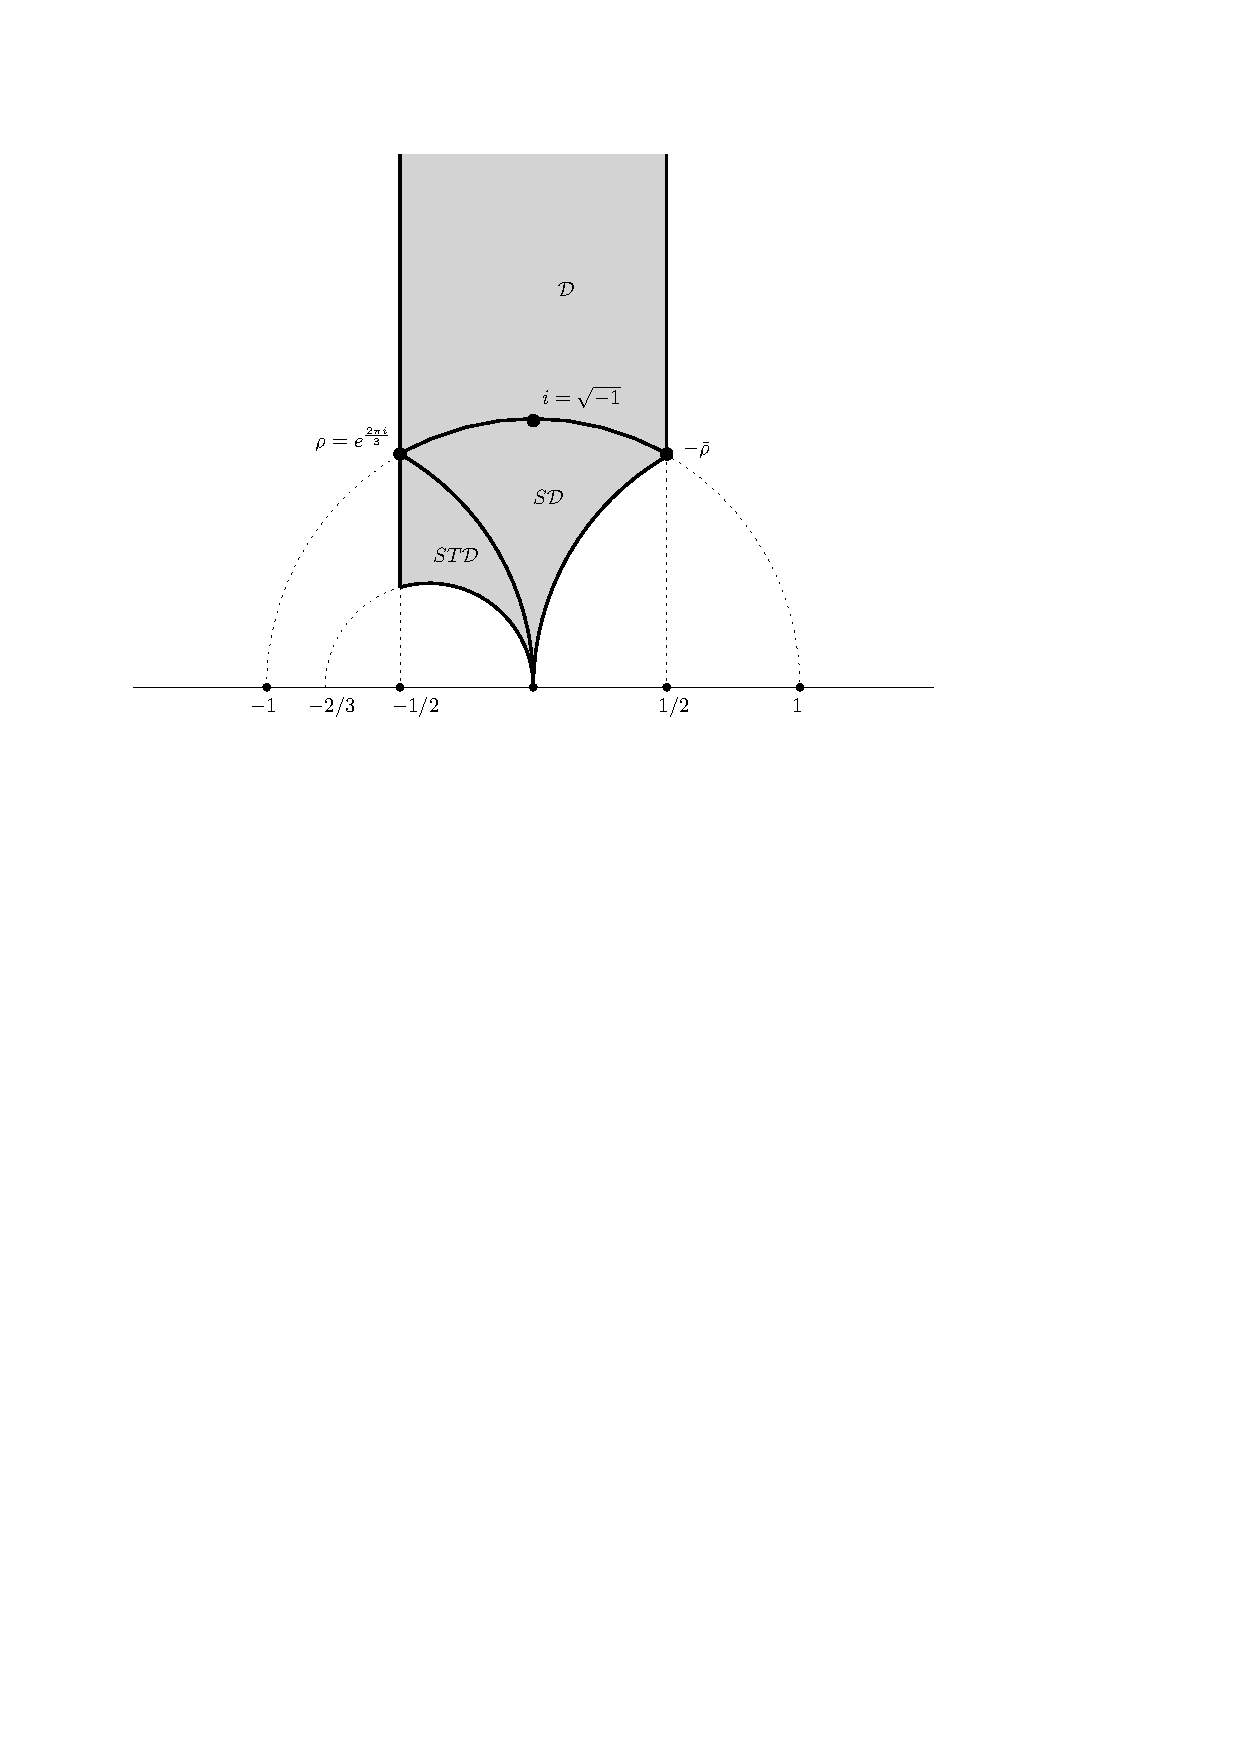
\includegraphics{fundomGamma02.pdf}
  \caption{A fundamental domain for $\Gamma_0(2)$}
  \label{fig:fundom-gamma02}
\end{figure}

In this case, the fundamental domain contains two points in its closure which do not belong to $\HH$: the cusp $\infty$ as before, but also $0$. The following result gives a construction of a fundamental domain for any congruence subgroup, using translates of the fundamental domain $\cD$ of $\SL_2(\ZZ)$ seen in Chapter~\ref{ch:modforms-full-level}.
\begin{proposition}
  Let $\Gamma$ be a congruence subgroup of $\SL_2(\ZZ)$. If there is a decomposition
\[
\Gamma\backslash \SL_2(\ZZ)=\bigcup_{h\in R} \Gamma h,\quad R\text{ finite,}
\]
then the set $\cD_\Gamma=\cup_{h\in R} h\cD$ is a (possibly non-connected) fundamental domain for $\Gamma$.
\end{proposition}
\begin{proof}
  If $z\in\HH$, then there exists $g\in\SL_2(\ZZ)$ and $z_0\in\cD$ such that $z = gz_0$. The coset decomposition implies that there is some $\gamma\in R$ and some $h\in \Gamma$ such that $g=h\gamma$. Therefore
\[
z = h\gamma z_0.
\]
Since $z_0'=\gamma z_0\in \gamma\cD\subset \cD_\Gamma$ we have written $z=h z_0'$ with $h\in\Gamma$.

It remains to be shown that if $z\in\stackrel{\circ}{\cD_\Gamma}$ and $\gamma z \in\stackrel{\circ}{\cD_\Gamma}$ for some $\gamma\in\Gamma$, then $\gamma = 1$. For that, let $\eps>0$ be small enough so that the ball $B_\eps(z)$ of radius $\eps$ around $z$ is fully contained in $\stackrel{\circ}{\cD_\Gamma}$. The ball $B_\eps(z)$ intersects some translates of $\cD$, say:
\[
B_\eps(z)\cap h\cD \neq \emptyset\iff h\in R'\subseteq R.
\]
Consider the translated ball $\gamma B_\eps(z)=B_\eps(\gamma z)$. Since $\gamma z$ is also in the interior of $\cD_\Gamma$, we deduce that $\gamma B_\eps(z)$ must intersect the interior of some translate of $\cD$, say $h\stackrel{\circ}{\cD}$, for some $h\in R$. Therefore:
\[
\gamma B_\eps(z)\cap h\stackrel{\circ}{\cD}\neq \emptyset \implies B_\eps(z)\cap \gamma^{-1}h\stackrel{\circ}{\cD}\neq \emptyset.
\]
Since we listed all the translates whose interior intersected with $B_\eps(z)$, we must have that $\gamma^{-1}h = h_0$. But now $\Gamma h = \Gamma \gamma^{-1}h = \Gamma h_0$, and since both $h$ and $h_0$ belong to $R$, we must have $h=h_0$. Therefore $\gamma^{-1}=1$, or $\gamma=1$ as we wanted.
\end{proof}

In order to further study the cusps, we consider the \emphh{rational projective line} $\PP^1(\QQ)=\QQ \cup\{\infty\}$. Note that $\SL_2(\ZZ)$ (in fact $\GL_2(\QQ)$) acts on $\PP^1(\QQ)$ by fractional linear transformations:
\[
\gamma x = \frac{ax +b}{cx+d},\quad \gamma = \mtx abcd\in\SL_2(\ZZ),x\in\PP^1(\QQ).
\]
Here we understand that $\gamma\infty = \frac ac$, and $\gamma x = \infty$ if $cx = -d$.

\begin{proposition}
  The action of $\SL_2(\ZZ)$ on $\PP^1(\QQ)$ is transitive, and it induces a bijection
\[
\SL_2(\ZZ)/\SL_2(\ZZ)_\infty\cong \PP^1(\QQ),\quad \SL_2(\ZZ)_\infty = \langle \pm T\rangle.
\]
\end{proposition}
\begin{proof}
  We will see that the orbit of $\infty$ is all of $\PP^1(\QQ)$, where we note that $\smtx abcd \infty = \frac ac$. Given $\frac ac\in\PP^1(\QQ)$ in reduced terms (that is, such that $(a,c)=1$), then B\'ezout's identity asserts the
existence of integers $b$ and $d$ such that $ad-bc=1$. Then the matrix $\smtx abcd$ belongs to $\SL_2(\ZZ)$ and takes $\infty$ to $\frac ac$.

The stabilizer of $\infty$, written $\SL_2(\ZZ)_\infty$, is:
\[
\SL_2(\ZZ)_\infty = \left\{\mtx abcd ~|~ \mtx abcd \infty = \infty\right\} = \left\{\mtx abcd ~|~ \frac ac = \infty\right\} = \left\{\mtx ab0d\right\} = \langle \pm T\rangle.
\]
\end{proof}

\begin{definition}
  The set of \emphh{cusps} of a congruence subgroup $\Gamma$ is the set $\Cusps(\Gamma)$ of $\Gamma$-orbits of $\PP^1(\QQ)$. Equivalently,
\[
\Cusps(\Gamma) = \Gamma\backslash \SL_2(\ZZ) / \SL_2(\ZZ)_\infty.
\]
\end{definition}

If $P = [\frac ac]$ is a cusp of $\Gamma$, set $\Gamma_P$ for the \emphh{stabilizer} of $P$ in $\Gamma$, the elements of $\Gamma$ fixing $P$.
\begin{lemma}
  If $\gamma_P(\infty) = P$, then
\[
\Gamma_P = \Gamma\cap \gamma_P\SL_2(\ZZ)_\infty \gamma_P^{-1}.
\]
\end{lemma}
\begin{proof}
 Let $\gamma\in\Gamma$. Then observe that
\begin{align*}
\gamma\in\Gamma_P&\iff \gamma P = P\iff \gamma \gamma_P\infty=\gamma_P\infty\\
&\iff \gamma_P^{-1}\gamma\gamma_P\infty=\infty\\
&\iff \gamma_P^{-1}\gamma\gamma_P\in \SL_2(\ZZ)_\infty\\
&\iff \gamma\in \gamma_P\SL_2(\ZZ)_\infty \gamma_P^{-1}.
\end{align*}
This concludes the proof.
\end{proof}

\begin{lemma}
The subgroup $H_P = \gamma_P^{-1}\Gamma\gamma_P\cap \SL_2(\ZZ)_\infty \subseteq \SL_2(\ZZ)_\infty$
does not depend on the choice of the representative for $P$, and has finite index in $\SL_2(\ZZ)_\infty$.
\end{lemma}
\begin{proof}
  Just note that if $\frac{a'}{c'}$ is another representative for $P$, then $\gamma_P$ gets modified into $\gamma\gamma_P$ for some $\gamma\in\Gamma$. Then $(\gamma\gamma_P)^{-1}\Gamma(\gamma\gamma_P) = \gamma_P^{-1}\Gamma\gamma_P$.
\end{proof}

\begin{lemma}
  Let $H$ be a subgroup of finite index in $\SL_2(\ZZ)_\infty$, and let $h$ be the index of $\{\pm 1\}H$ in $\SL_2(\ZZ)_\infty$. Then $H$ is one of he following:
\[
H = \begin{cases}
\langle \smtx 1h01\rangle&\\
\langle \smtx{-1}{h}{0}{-1}\rangle&\\
\{\pm 1\}\times \langle \smtx 1h01\rangle&
\end{cases}
\]
\end{lemma}
\begin{proof}
  Exercise.
\end{proof}
\begin{definition}
The integer $h_\Gamma(P)=h$ in the above lemma is called \emphh{width of a cusp} $P$ for $\Gamma$. A cusp is an \emphh{irregular cusp} if $\gamma_P^{-1}\Gamma_P\gamma_P$ is of the form $\langle \smtx{-1}{h}{0}{-1}\rangle$, and it is \emphh{regular cusp} otherwise.
\end{definition}

\begin{example}
  In this example we show that if $p$ is any prime, then $\Cusps(\Gamma_0(p)) = \{ \infty, 0\}$.

Write an element $\gamma\in\Gamma_0(p)$ as $\smtx{a}{b}{pc}{d}$, with $a,b,c,d\in\ZZ$ satisfying $ad-pbc =1$. The orbit of $\infty$ is:
\[
\Gamma_0(p)\cdot \infty = \left\{\mtx{a}{b}{pc}{d}\infty\right\} = \left\{\frac{a}{pc}~\colon~ a,c\in\ZZ,\gcd(a,pc) = 1\right\} = \left\{ \frac{r}{s}~\colon~ p\mid s, \gcd(r,s)=1\right\}.
\]
We thus see the orbit of the cusp $\infty$ consists of infinity together with all the rationals which when expressed in reduced terms have a denominator which is divisible by $p$. One element which is not in this orbit is $0=\frac{0}{1}$. Let us study then the orbit of $0$.
\[
\Gamma_0(p) \cdot 0 = \{\mtx{a}{b}{pc}{d} 0\} = \{\frac{b}{d}~\colon~ b,d\in\ZZ, \gcd(b,d)=1, p\nmid d\}.
\]
\end{example}
As we have seen in the example above, each cusp may have a different width. However, if $\Gamma$ is a normal congruence subgroup of $\SL_2(\ZZ)$, the subgroup $H_P$ does not depend on the cusp $P$ and hence all cusps have the same width and regularity.

Although one can have more cusps than the index of $\Gamma$, the last result of this section says that this is basically right, once one counts in a proper way. To prove it, we will need a group-theoretic result.

\begin{lemma}[orbit--stabilizer for infinite groups]
  \label{lemma:orbit-stabilizer}
Let $G$ be a group acting transitively on a set $X$ and let $H$ be a finite index subgroup of $G$. Then for any $x\in X$ the stabilizer of $x$ in $H$ has finite index in the stabilizer of $x$ in $G$, and the following formula holds:
\[
\sum_{x\in H\backslash X} [G_x\colon H_x]=[G\colon H].
\]
\end{lemma}
\begin{proof}
  Let $x\in X$, and consider the inclusion map $G_x\to G$. By taking the quotient by $H$ we get $G_x\to H\backslash G$. Suppose $g_1, g_2$ are mapped to the same element $Hg$ in $H\backslash G$. This means that $Hg_1 = Hg_2$, or that $g_2g_1^{-1}$ belongs to $H$. Since $g_2g_1^{-1}$ stabilizes $x$ as well, we deduce that $H_x g_1 = H_x g_2$. Therefore there is an injection of $H_x\backslash G_x\injects H\backslash G$. Since by assumption the latter set is finite, so is the first. Note also that the image of the map is precisely $H\backslash HG_x$, and thus we also obtain $[G_x\colon H_x] = [H G_x\colon H]$.

To prove the second assertion, fix an element $x_0\in X$, and consider the map
\[
H\backslash G\tto H\backslash X,\quad Hg\mapsto Hgx_0
\]
which is surjective because $G$ acts transitively on $X$. The fibre $T_{Hx}$ of an orbit $Hx$ consists of the set of classes $Hg$ such that $Hgx_0 = Hx$. Let $g_x\in G$ be such that $g_x x_0 = x$. Write $Hg = Hg'g_x$ and then we have:
\begin{align*}
T_{Hx}&\cong \{Hg'\in H\backslash G\colon Hg'g_xx_0 = Hx\} = \{Hg'\in H\backslash G\colon Hg'x=Hx\}= H\backslash(H G_x)\cong H_x\backslash G_x.
\end{align*}
This allows us to find a formula for $[G\colon H]$:
\begin{align*}
[G\colon H]&=\# (H\backslash G) = \sum_{x\in R} \# T_{Hx} = \sum_{x\in R} [G_x\colon H_x].
\end{align*}
\end{proof}

\begin{theorem}
  Let $\Gamma$ be a congruence subgroup. Then we have
\[
\sum_{P\in \Cusps(\Gamma)} h_\Gamma(P) = [\SL_2(\ZZ)\colon \{\pm 1\}\Gamma].
\]
\end{theorem}
\begin{proof}
  Consider the group $G=\PSL_2(\ZZ)=\SL_2(\ZZ)/\{\pm 1\}$, which acts transitively on the set $X=\PP^1(\QQ)$. Let $H$ be the image of $\Gamma$ in $G$. Note that $H\backslash X=\Cusps(\Gamma)$. Also, $G_\infty$ is the image in $G$ of $\SL_2(\ZZ)_\infty$. For each $x\in X$, let $\gamma\in G$ be such that $\gamma \infty = x$. Then
\[
G_x=\gamma G_\infty\gamma^{-1},\text{ and}\quad H_x= \gamma \left(\gamma^{-1}H\gamma\right)_\infty \gamma^{-1}.
\]
Therefore
\[
[G_x\colon H_x] = [\bar\SL_2(\ZZ)\colon \bar \Gamma_P] = h_\Gamma(P),
\]
where by $\ol{(\cdot)}$ we write the image of the group inside $G$. Then applying Lemma~\ref{lemma:orbit-stabilizer} to this setting gives
\[
\sum_{P\in \Cusps(\Gamma)} h_\Gamma(P) = [G\colon H] = [\SL_2(\ZZ)\colon \{\pm 1\}\Gamma].
\]
\end{proof}
\section{Fourier expansion at infinity}
\label{sec:fourier-expansion-at-infinity}

Let $\Gamma$ be a congruence subgroup of level $N$. Note that the matrix $\smtx 1N01$ belongs to $\Gamma(N)$, and thus there is a minimum $h>0$ with the property that $\smtx 1h01 \in\Gamma$.
\begin{definition}
  The \emphh{fan width} of $\Gamma$ is the minimum $h>0$ such that $\smtx 1h01\in\Gamma$.
\end{definition}
\begin{remark}
  The fan width of a congruence subgroup of level $N$ is a divisor of $N$.
\end{remark}
Write
\[
q_h =q_h(z)= e^{\frac{2\pi i z}{h}},
\]
and note that $z\mapsto q_h(z)$ is periodic with period $h$. Define $g$ by $g = f\circ q_h^{-1}$.
That is, $g(q_h) = f(z)$. Although $q_h$ is not invertible, the above definition makes sense, and $g$ has
a Laurent expansion.
\begin{definition}
  The $q$-expansion of $f$ at infinity is the Laurent expansion:
\[
f(z) = g(q_h)=\sum_{n=-\infty}^\infty a(n)q_h^n.
\]
\end{definition}

\section{Expansions at cusps}
\label{sec:expansions-at-cusps}


Let $s$ be a cusp, $s\neq \infty$. Write $s =\alpha\infty$ for some $\alpha\in\SL_2(\ZZ)$, and consider the equation:
\[
f(\alpha z) = j(\alpha,z)^{k}(f|_k\alpha)(z).
\]
 Since $j(\alpha,z)\neq 0,\infty$ when $z$ is near $\infty$, the behavior of $f(z)$ near $s$  is related to the behavior of $(f|_k\alpha)(z)$ near $\infty$. Assume that $f$ is weakly modular for the congruence subgroup $\Gamma$. Since\[
(f|_k\alpha)|_k(\alpha^{-1}\gamma\alpha) = (f|_k\gamma)|_k\alpha = f|_k\alpha,
\]
the new function $f|_k\alpha$ is invariant under the group $\Gamma'=\alpha^{-1}\Gamma\alpha$. Since $\Gamma(N)$ is normal inside $\SL_2(\ZZ)$, we deduce that $\Gamma'$ is also a congruence subgroup of level $N$. Hence $f|_k\alpha$ has a Fourier expansion at infinity as in Section~\ref{sec:fourier-expansion-at-infinity} in powers of $q_N$.
\begin{definition}
  The \emphh{expansion of $f$ at a cusp} $s$ is the expansion:
\[
f|_k\alpha = \sum_{n=-\infty}^\infty b(n)q_N^n.
\]
\end{definition}

\section{Definition of modular forms}
The expansions at different cusps allow us to define modular forms for arbitrary congruence subgroups.
\begin{definition}
\label{def:modforms-congruence}
  A function $f\colon\HH\to\CC$ is a \emphh{modular form} of weight $k$ for a congruence subgroup $\Gamma$ if:
  \begin{enumerate}
  \item $f$ is holomorphic on $\HH$,
  \item $f|_k\gamma = f$ for all $\gamma\in\Gamma$, and
  \item $f|_k\alpha$ is holomorphic at infinity for all $\alpha\in\SL_2(\ZZ)$.
  \end{enumerate}
 A function is a \emphh{cusp form} of weight $k$ for a congruence subgroup $\Gamma$ if instead of $3$ is satisfies:
 \begin{enumerate}[resume]
\item[3'.] $f|_k\alpha$ vanishes at infinity for all $\alpha\in\SL_2(\ZZ)$.
 \end{enumerate}
The \emphh{space of modular forms} of weight $k$ for a congruence subgroup $\Gamma$ is written $M_k(\Gamma)$; the \emphh{space of cusp forms} of weight $k$ for a congruence subgroup $\Gamma$ is written $S_k(\Gamma)$.
\end{definition}
\begin{proposition}
  Suppose that $f\colon\HH\to\CC$ satisfies $1$ and $2$ above. Suppose that $f$ is holomorphic at infinity. That is,
\[
f(z) = \sum_{n=0}^\infty a(n)q_N^n.
\]
Furthermore, suppose that there exists constants $C>0$ and $r>0$ such that:
\[
|a(n)|< Cn^r,\quad \forall n > 0.
\]
Then $f$ satisfies $3$, and thus $f\in M_k(\Gamma)$.
\end{proposition}
\begin{proof}
  Exercise.
\end{proof}
\begin{remark}
  In fact, the converse is also true: if the Fourier coefficients of $f$ grow as $Cn^r$ as above, then condition $3$ in Definition~\ref{def:modforms-congruence} is satisfied. The proof of this fact uses Eisenstein series for congruence subgroups, and thus will be postponed until we introduce those.
\end{remark}

\begin{example}
  Let $f$ be a weakly-modular form of weight $k$ for the full modular subgroup. Consider the function $g(z) = f(Nz)$. If $\gamma\in\Gamma_0(N)$ is of the form $\gamma=\smtx abcd$, then since $N\mid c$ the matrix
\[
\gamma'=\mtx a{bN}{c/N}{d}
\]
is in $\SL_2(\ZZ)$. Therefore we may compute:
\begin{align*}
g(\gamma z) &= f(N(\gamma z)) = f(\frac{Naz+bN}{cz+d}) \\
&= f(\frac{a(Nz)+bN}{c/N (Nz) + d}) = f(\gamma'(Nz))\\
&=(c/N(Nz) + d)^{k}f(Nz) = j(\gamma,z)^k g(z).
\end{align*}
Therefore the function $g$ is weakly-modular of weight $k$ for the congruence subgroup $\Gamma_0(N)$. In fact, this operation defines injections
\[
M_k(\SL_2(\ZZ))\to M_k(\Gamma_0(N))
\]
which will play an important role later in the course, in the Atkin-Lehner-Li theory of old/new forms.
\end{example}

We end this section by realizing that the definition of modular forms can be checked by finitely many computations. Suppose that $\sigma=\alpha\infty$ and $\tau=\beta\infty$ are two cusps (here $\alpha$ and $\beta$ are in $\SL_2(\ZZ)$). Suppose that $\sigma=\gamma\tau$ with $\gamma\in\Gamma$.
\begin{proposition}
If
\[
f|_k\alpha = \sum_{n=-\infty}^\infty a(n)q_h^n,
\]
then
\[  f|_k\beta = \sum_{n=-\infty}^\infty b(n)q_h^n,\quad b(n) = (\pm 1)^k e^{\frac{2\pi i n j}{h}} a(n), j\in \ZZ.
\]
\end{proposition}
\begin{proof}
  By assumption $\alpha\infty=\gamma\beta\infty$, so $\alpha^{-1}\gamma\beta\infty=\infty$, and therefore since the only matrices that fix infinity are of the form $\pm \smtx 1j01$ we have:
\[
\alpha^{-1}\gamma\beta = \pm\mtx 1j01,\quad j\in\ZZ.
\]
This means that
\[
\beta = \pm \gamma^{-1}\alpha\mtx 1j01,
\]
and therefore:
\begin{align}
f|_k\beta &= f|_k\pm I |_k \gamma^{-1} |_k\alpha |_k \mtx 1j01 = (\pm 1)^k\sum a(n)e^{\frac{2\pi i n z}{h}} |_k \mtx 1j01\\
&=(\pm 1)^k\sum a(n) e^{\frac{2\pi i n (z+j)}{h}}.
\end{align}
\end{proof}
\begin{corollary}
  For each $n\in\ZZ$, we have $a(n)=0$ if and only if $b(n)=0$. In particular, it is enough to check $3$ or $3'$ for one representative from each of the equivalence classes of cusps.
\end{corollary}

\section{Valence formula for congruence subgroups}

  Let $\Gamma$ be a congruence subgroup of level $N$. In order to state the next result we need to define the order of a weakly-modular function at a cusps $P\in\Cusps(\Gamma)$.
\begin{definition}
  Let $f$ be a weakly-modular form of weight $k$ for $\Gamma$, and let $P$ be a cusp of $\Gamma$ of width $h_\Gamma(P)$. Since $f(z+N)=f(z)$, we can write $f$ as a Laurent series in $q_N=e^{\frac{2\pi i z}{N}}$, say
\[
f(q_N) = \sum_{n\geq n_0} a_n q_N^n,\quad a_{n_0}\neq 0.
\]
The \emphh{order of vanishing} of $f$ at $P$ is $v_P(f) = \frac{h_\Gamma(P)}{N}n_0$.
\end{definition}

Here is a generalization of Theorem~\ref{thm:valence-formula} to arbitrary congruence subgroups.
\begin{theorem}[valence formula for congruence subgroups]
  Let $\Gamma$ be a congruence subgroup, and let $k$ be an integer. Let $f$ be a non-zero meromorphic function on $\HH\cup\{\infty\}$, which is weakly-modular of weight $k$ for $\Gamma$. Then we have
\[
\sum_{z\in\Gamma\backslash\HH} \frac{v_z(f)}{\#\ol\Gamma_z} +\sum_{P\in\Cusps(\Gamma)} v_P(f)=\frac{k}{12}[\PSL_2(\ZZ)\colon\ol\Gamma].
\]
\end{theorem}
\begin{proof}
  Write $d_\Gamma=[\PSL_2(\ZZ)\colon\ol\Gamma]$, let $R$ be a set of coset representatives for $\ol\Gamma\backslash\PSL_2(\ZZ)$, and define $F=\prod_{\gamma\in R} f|_k\gamma$. Note that $F$ is weakly-modular of weight $kd_\Gamma$ for $\SL_2(\ZZ)$, and it is meromorphic at $\infty$. By Theorem~\ref{thm:valence-formula} we have
\[
v_\infty(F)+\frac 12 v_i(F) + \frac 13 v_\rho(F) +\sum_{w\in W} v_w(F) = \frac{k}{12} d_\Gamma.
\]
Another way to write the above is:
\[
 v_\infty(F) + \sum_{z\in\PSL_2(\ZZ)\backslash\HH} \frac{v_z(F)}{\#\PSL_2(\ZZ)_z} = \frac{k}{12} d_\Gamma.
\]
We may now compute:
\begin{align*}
v_z(F) &= \sum_{\gamma\in\ol\Gamma\backslash\PSL_2(\ZZ)} v_z(f|_k\gamma) = \sum_{\gamma\in\ol\Gamma\backslash\PSL_2(\ZZ)} v_{\gamma z}(f)=\sum_{w\in\ol\Gamma\backslash \PSL_2(\ZZ)z} [\PSL_2(\ZZ)_w\colon\ol\Gamma_w] v_w(f).
\end{align*}
The last equality follows by grouping all elements $\gamma$ such that $\gamma z=w$, for each possible $w$. Now, since $\PSL_2(\ZZ)_w$ is finite and independent of $w\in \ol\Gamma\backslash\PSL_2(\ZZ)z$, we get
$[\PSL_2(\ZZ)_w\colon\ol\Gamma_w]=\frac{\# \PSL_2(\ZZ)_z}{\#\ol\Gamma_w}$.
Dividing by $\#\PSL_2(\ZZ)_z$ we obtain
\[
\frac{v_z(F)}{\#\PSL_2(\ZZ)_z} = \sum_{w\in \ol\Gamma\backslash \PSL_2(\ZZ)z} \frac{v_w(f)}{\#\ol\Gamma_w}.
\]
By summing over a set of representatives for $\PSL_2(\ZZ)\backslash \HH$ we finally obtain
\begin{align*}
\sum_{z\in\PSL_2(\ZZ)\backslash\HH} \frac{v_z(F)}{\#\PSL_2(\ZZ)_z} &=\sum_{z\in\PSL_2(\ZZ)\backslash \HH}\sum_{w\in\ol\Gamma\backslash \PSL_2(\ZZ)z} \frac{v_w(f)}{\#\ol\Gamma_w}=\sum_{w\in\ol\Gamma\backslash\HH} \frac{v_w(f)}{\#\ol\Gamma_w}.
\end{align*}
In order to conclude the proof it remains to be shown that $v_\infty(F) = \sum_{P\in\Cusps(\Gamma)} v_P(f)$. We first prove it assuming that $\ol \Gamma$ is normal in $\PSL_2(\ZZ)$. In this case, we have
\begin{align*}
d_\Gamma v_\infty(F) &= \sum_{P\in\Cusps(\Gamma)} h_\Gamma(P)v_\infty(F)\\
&=\sum_{P\in\Cusps(\Gamma)} v_P(F)\\
&=\sum_{P\in\Cusps(\Gamma)} \sum_{\gamma\in R} v_{\gamma P}(f)\\
&=\sum_{P\in\Cusps(\Gamma)} \sum_{P'\in\Cusps(\Gamma)} \#\{\gamma\in R ~|~ \gamma P = P'\} v_{P'}(f)\\
&=\sum_{P'\in\Cusps(\Gamma)} \sum_{P\in\Cusps(\Gamma)} \#\{\gamma\in R ~|~ \gamma P = P'\} v_{P'}(f)\\
&=d_\Gamma\sum_{P'\in\Cusps(\Gamma)} v_{P'}(f).
\end{align*}
Note that any congruence subgroup $\Gamma$ contains a subgroup (for instance $\Gamma(N)$) which is normal in $\SL_2(\ZZ)$, and such that it is of finite index. Therefore it is enough to show that, if $\Gamma'\subset \Gamma$ have finite index and $g$ is weakly modular of weight $k$ for $\Gamma$, then
\[
\sum_{P'\in \Cusps(\Gamma')} v_{P'}(f) = \frac{d_{\Gamma'}}{d_\Gamma} \sum_{P'\in \Cusps(\Gamma')} v_{P'}(f).
\]
Let $P\in\Cusps(\Gamma)$ and $P'\in\Cusps(\Gamma')$ be such that $[P]=[P']$ inside $\Cusps(\Gamma)$. Pick $\sigma\in\SL_2(\ZZ)$ such that $\sigma\infty = [P]$ in $\Cusps(\Gamma)$. Write also $n_0 = v_P^\Gamma(g)$, and $m = \frac{h_{\Gamma'}}{h_\Gamma}$. Then:
\[
(g|_k\sigma)(z) = \sum_{n\geq n_0} a_n(g) e^{\frac{2\pi i n z}{h_\Gamma}} = \sum_{n\geq n_0} a_n(g)e^{\frac{2\pi i nmz}{h_{\Gamma'}}} = \sum_{n\geq mn_0} a_n(g)e^{\frac{2\pi i nz}{h_{\Gamma'}}}.
\]
Hence we have $v_{P'}(g) = m v_P(g)$, as we wanted. This concludes the proof of the valence formula.
\end{proof}

As for level $1$, the valence formula gives a criterion for equality of modular forms:
\begin{corollary}
  Let $f$ and $g$ be two modular forms in $M_k(\Gamma)$, whose $q$-expansions (at one cusp of $\Gamma$) coincide up to the term $\frac{k}{12}[\PSL_2(\ZZ)\colon\ol\Gamma]$. Then $f$ and $g$ are equal.
\end{corollary}

There are dimension formulas for congruence subgroups (see~\cite[Chapter 3]{diamond-shurman}) but we will not see them in this course.


%%% Local Variables: 
%%% mode: latex
%%% TeX-master: "main"
%%% End: 


\chapter{Complex Tori}
\label{chap:complextori}

In this chapter we reinterpret modular forms as functions on certain very interesting geometric objects.

\section{Lattices and tori}
\begin{definition}
  A \emphh{lattice} is a free $\ZZ$-module $\Lambda$ of rank $2$ inside $\CC$ which contains an $\RR$-basis for $\CC$. Concretely, $\Lambda = \ZZ\omega_1\oplus \ZZ\omega_2$, where $\omega_1$ and $\omega_2$ are $\RR$-linearly independent complex numbers. We will always assume that $\omega_1/\omega_2\in\HH$, which can always be accomplished by possible swapping them.
\end{definition}

As you know, in general there are many choices for a basis of a given submodule.
\begin{proposition}
\label{prop:nine}
  Suppose that $\Lambda=\langle \omega_1,\omega_2\rangle$ and $\Lambda'=\langle \omega_1',\omega_2'\rangle$. Then $\Lambda = \Lambda'$ if and only if there exists $\gamma\in\SL_2(\ZZ)$ such that
\[
\mat{\omega_1\\\omega_2} = \gamma\mat{\omega'_1\\\omega'_2}.
\]
\end{proposition}
\begin{proof}
  Exercise.
\end{proof}

Lattices become interesting when we quotient $\CC$ out by them.
\begin{definition}
  A \emphh{complex torus} is the set $\CC/\Lambda =\{z+\Lambda~|~ z\in\CC\}$. It has the structure of an abelian group, and analytically it is a torus (a genus one Riemann surface).
\end{definition}
\begin{figure}
\begin{center}
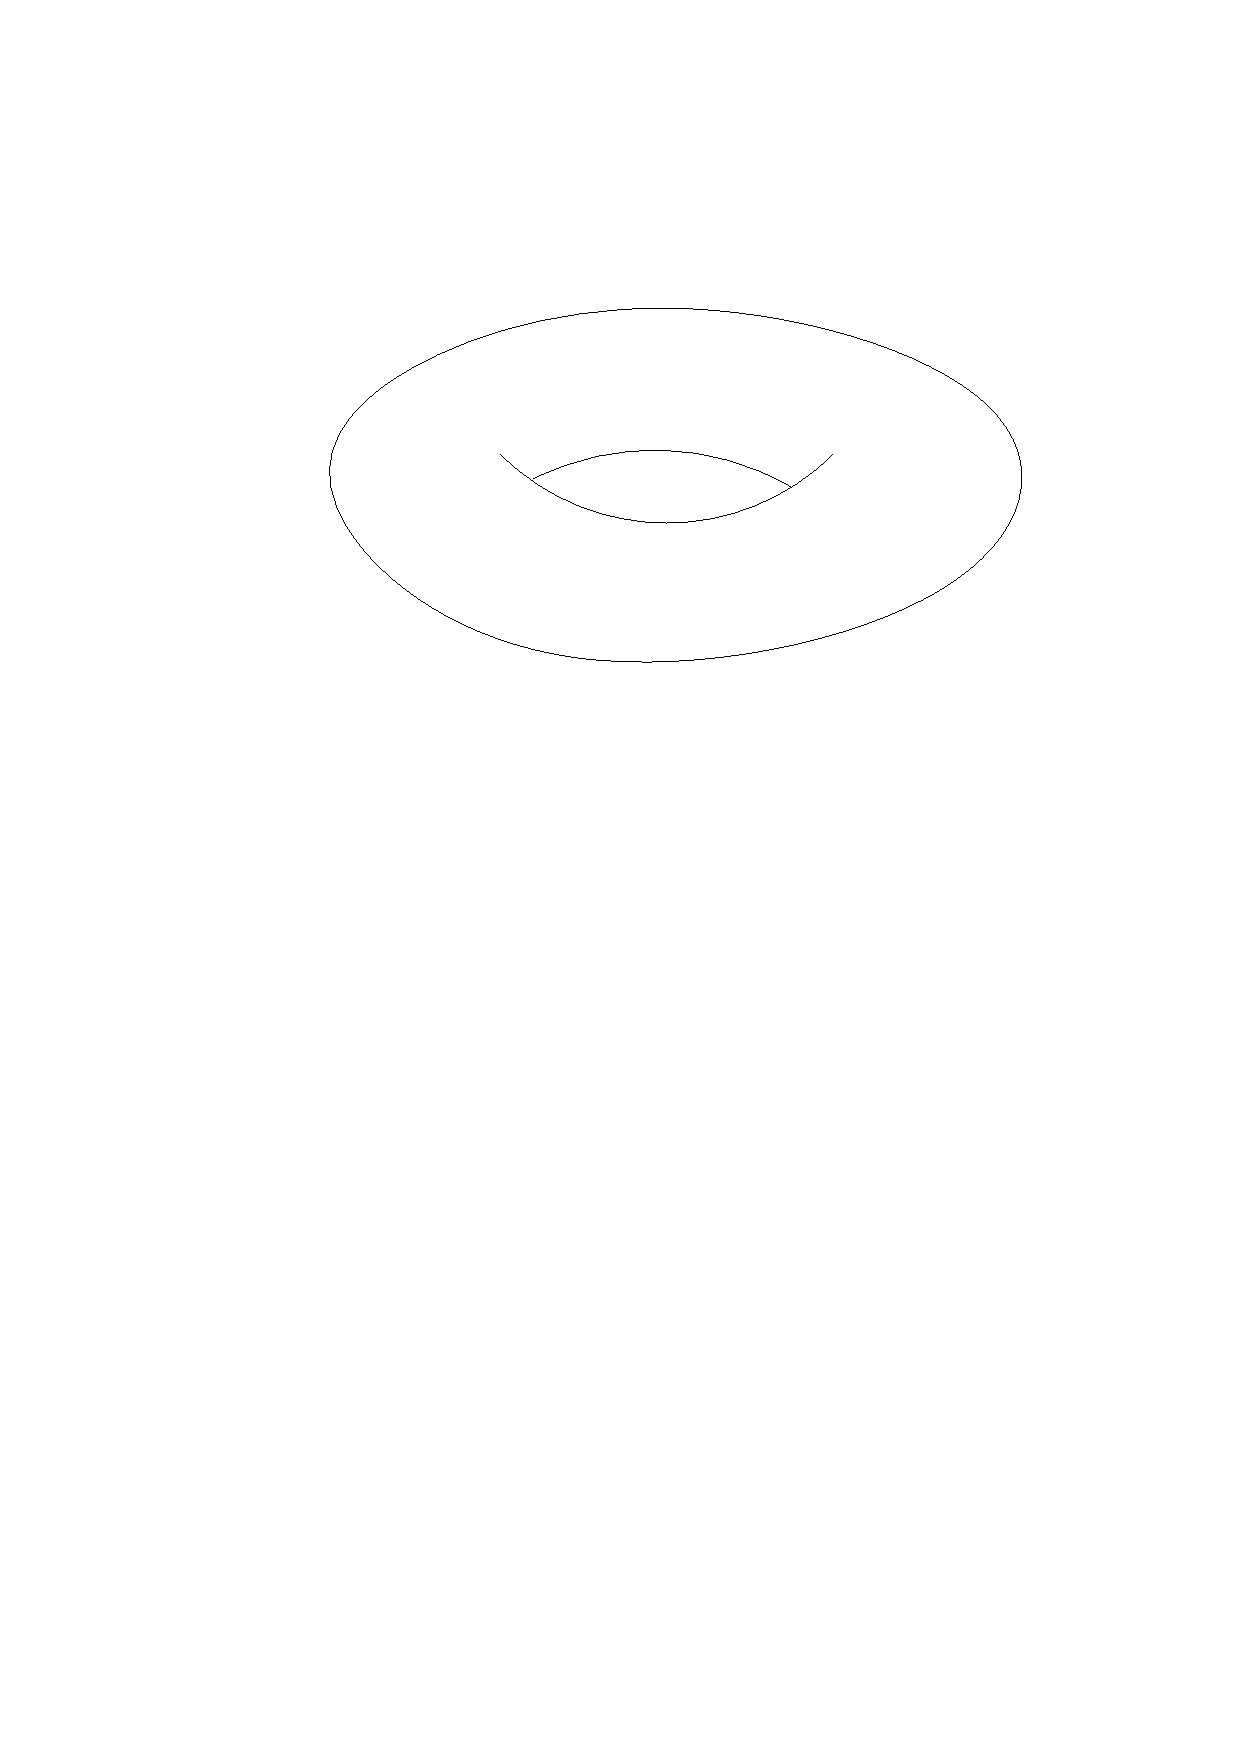
\includegraphics[height=3cm]{torus.pdf}
\end{center}
\label{fig:torus}
\end{figure}
\begin{proposition}
  Suppose that $\varphi\colon\CC/\Lambda\to\CC/\Lambda'$ is a holomorphic map. Then there exist complex numbers $m$ and $b$ such that:
  \begin{enumerate}
  \item $m\Lambda\subseteq \Lambda'$, and
  \item $\varphi(z+\Lambda)=mz+b+\Lambda'$.
  \end{enumerate}
Moreover, $\varphi$ is invertible if and only if $m\Lambda=\Lambda'$.
\end{proposition}
\begin{proof}
 The complex plane $\CC$ is the universal covering space of $\CC/\Lambda$ and $\CC/\Lambda'$. Therefore, $\varphi$ can be lifted to a map $\tilde\varphi\colon\CC\to\CC$. Suppose now that $\lambda\in\Lambda$, and define
\[
f_\lambda(z)=\tilde\varphi(z+\lambda)-\tilde\varphi(z).
\]
\begin{figure}[h]
  \centering
  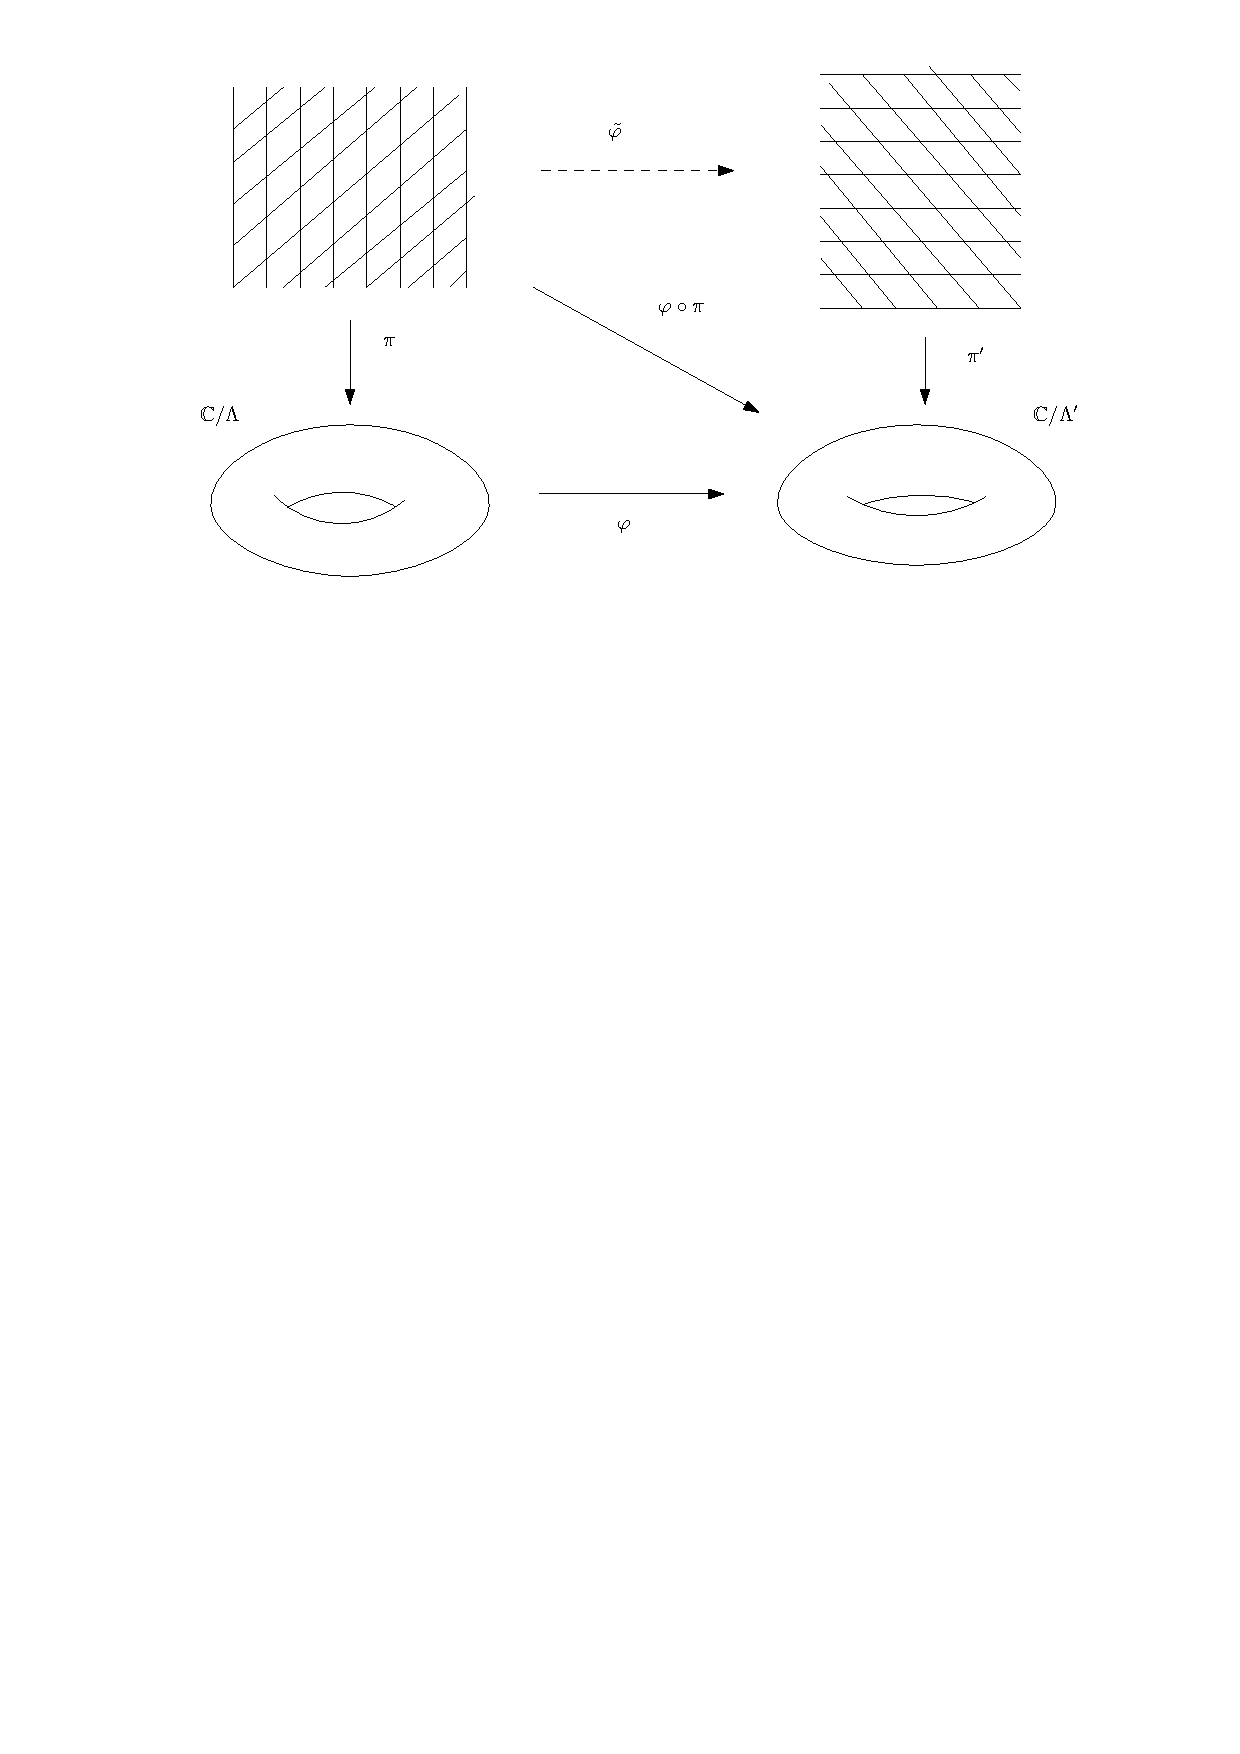
\includegraphics[height=5cm]{Pictures/universal_covering_space.pdf}

  \caption{Lifting to the universal covering space}
  \label{fig:universal-covering-space}
\end{figure}
Then $f_\lambda$ is continuous and has image in $\Lambda'$. Since $\Lambda'$ is discrete, necessarily $f_\lambda$ is constant. Consider the derivative. For each $\lambda\in\Lambda$, we have
\[
\tilde\varphi'(z+\lambda)=\tilde\varphi'(z).
\]
Therefore $\tilde\varphi'(z)$ is holomorphic and doubly-periodic, hence bounded. By Liouville's theorem, $\tilde\varphi'$ is constant. We deduce that $\tilde\varphi(z)=mz+b$, as wanted.
\end{proof}

\begin{corollary}
  Let $\varphi\colon\CC/\Lambda\to\CC/\Lambda'$ be a holomorphic map. Then $\varphi$ is a group homomorphism if and only if $\varphi(0)=0$, if and only if $b\in\Lambda'$.
\end{corollary}

\begin{remark}
  If $\varphi$ as above is a holomorphic group isomorphism, then necessarily $m\Lambda=\Lambda'$ and also $\varphi(z+\Lambda)=mz+\Lambda'$.
\end{remark}

Here are two examples of possible maps like the ones above.
\begin{example}
  The map \emphh{multiplication-by-$N$}, usually written $[N]$, is a homomorphism:
\[
\xymatrix@R5pt{\CC/\Lambda\ar[r]^{[N]}&\CC/\Lambda\\
z+\Lambda\ar@{|->}[r]&Nz+\Lambda
}
\]
The kernel of $[N]$ is the group of $N$-torsion points, isomorphic to $\ZZ/N\ZZ\times\ZZ/N\ZZ$.
\end{example}

\begin{example}
  Consider $\Lambda=\ZZ\omega_1\oplus\ZZ\omega_2$. Define $\tau=\omega_1/\omega_2\in \HH$, and set $\Lambda_\tau=\ZZ\tau\oplus\ZZ$. Then $\CC/\Lambda\cong \CC/\Lambda_\tau$.
\end{example}

The previous example can be brought a little bit further as follows.
\begin{lemma}
  The complex tori $\CC/\Lambda_\tau$ and $\CC/\Lambda_{\tau'}$ are isomorphic if and only if $\tau=\gamma\tau'$ for some $\gamma\in\SL_2(\ZZ)$.
\end{lemma}
\begin{proof}
  Suppose that
\[
\tau=\gamma\tau'=\frac{a\tau'+b}{c\tau'+d}.
\]
Let $m=c\tau'+d$. Then $m\Lambda_\tau = \ZZ(a\tau'+b)\oplus\ZZ(c\tau'+d)$. By Proposition~\ref{prop:nine}, this lattice is the same as $\ZZ\tau'\oplus\ZZ=\Lambda_{\tau'}$. The other direction is obtained by reading the equalities in reverse.
\end{proof}
\begin{remark}
  We have just seen that there is a ``natural bijection'' between isomorphism classes of tori and elements $\tau\in\SL_2(\ZZ)\backslash\HH$. This innocent statement is \textbf{really} important.
\end{remark}

\begin{example}[Eisenstein series attached to a lattice]
  Let $\Lambda$ be a lattice. Define, for $k>2$ even,
\[
G_k(\Lambda)=\sumprime_{\omega\in\Lambda}\omega^{-k}.
\]
Note that $G_k(\Lambda_\tau) = G_k(\tau)$ is the usual Eisenstein series defined in the previous chapter. The transformation law reads in this case:
\[
G_k(m\Lambda)=m^{-k}G_k(\Lambda).
\]
\end{example}
\section{Tori and elliptic curves}
The next goal is to relate $\CC/\Lambda$ to elliptic curves. This will allow to think of modular forms as functions either on lattices or on elliptic curves.

\subsection{Meromorphic functions on \texorpdfstring{$\CC/\Lambda$}{C/L}}
\label{sec:meromorphic-functions-CmodLambda}

Let $\CC(\Lambda)$ be the field of meromorphic functions on $\CC/\Lambda$. That is, meromorphic functions $f\colon\CC\to\CC$ satisfying $f(z+\lambda)=f(z)$ for all $\lambda\in\Lambda$.
\begin{proposition}
  Let $f\in\CC(\Lambda)$. Then:
  \begin{enumerate}
  \item $\sum_{z\in\CC/\Lambda} \res_z f = 0$.
  \item $\sum_{z\in\CC/\Lambda} \ord_z f = 0$.
  \item $\sum_{z\in\CC/\Lambda} z\ord_z f\in\Lambda$.
  \end{enumerate}
\end{proposition}
\begin{proof}
  Consider a fundamental parallelepiped $D$ which misses all zeroes and poles. This can be done because zeroes and poles form a discrete set. Now one can compute the quantities
\[
\frac{1}{2\pi i} \int_{\partial D} f(z)dz,\quad \frac{1}{2\pi i} \int_{\partial D} \frac{f'(z)}{f(z)}dz\quad, \text{and }\frac{1}{2\pi i} \int_{\partial D} \frac{zf'(z)}{f(z)}dz.
\]
\end{proof}
\begin{definition}
  The \emphh{order of a meromorphic function} $f$ is the number $\ord(f)$ of zeroes (which equals the number of poles) of $f$, when counted with multiplicities.
\end{definition}
Note that the first statement in the above proposition implies that $\ord(f)\geq 2$.

\subsection{The Weierstrass \texorpdfstring{$\wp$}{P}-function}
\label{sec:weierstrass-pe}

Consider the following function:
\[
\wp_\Lambda(z)=\frac{1}{z^2}+\sumprime_{w\in\Lambda} \left(\frac{1}{(z-w)^2} - \frac{1}{w^2}\right).
\]
It is immediate to see that $\wp_\Lambda$ is an even function, which converges absolutely and uniformly on compact sets away from $\Lambda$.
\begin{lemma}
  The function $\wp_\Lambda$ is $\Lambda$-periodic.
\end{lemma}
\begin{proof}
  Note that the derivative of $\wp_\Lambda$ is
\[
\wp_\lambda'(z)=-2\sum_{w\in\Lambda} \frac{1}{(z-w)^3},
\]
which is clearly $\Lambda$-periodic. Set $f(z)=\wp_\Lambda(z+w_1)-\wp_\Lambda(z)$, where $w_1\in\Lambda$. Then $f'(z)=0$, so $f$ is constant, say $f(z)=c$. To determine $c$, set $z=-\frac{w}{2}$ and note that since $\wp_\Lambda$ is even, we get
\[
c=\wp_\Lambda(w_1/2)-\wp_\Lambda(-w_1/2) = 0.
\]
Therefore $f(z)=0$, and thus $\wp_\Lambda$ is $\Lambda$-periodic.
\end{proof}

The lemma gives that $\wp_\lambda(z)$ belongs to $\CC(\Lambda)$. In fact, $\CC(\Lambda)$ is generated by $\wp_\Lambda$ and $\wp'_\Lambda$, but we are not going to prove this here.

\begin{proposition}
  The Laurent expansion of $\wp_\Lambda(z)$ at $z=0$ is
\[
\wp_\Lambda(z) = \frac{1}{z^2} + \sum_{n\geq 2,\text{ even}} (n+1)G_{n+2}(\Lambda)z^{n},
\]
and it has radius of convergence equal to the lattice point closest to the origin.
\end{proposition}
\begin{proof}
  See~\cite[Proposition 1.4.1]{diamond-shurman}.
\end{proof}

These expansions allow us to find algebraic relations between $\wp_\Lambda$ and $\wp'_\Lambda$. Since
\[
\wp_\Lambda = \frac{1}{z^2}+3G_4(\Lambda)z^2+O(z^4)
\]
and
\[
\wp'_\Lambda = \frac{-2}{z^3} + 6G_4(\Lambda)z + O(z^3),
\]
we deduce:
\[
(\wp_\Lambda')^2=\frac{4}{z^6}+O(z^{-2}) = 4(\wp_\Lambda)^3 + O(z^{-2}).
\]
We can work with a couple more terms of the expansions, to get:
\[
(\wp_\Lambda')^2 = 4(\wp_\Lambda)^3-60G_4(\Lambda)\wp_\Lambda-140G_6(\Lambda)+F(z),\quad F(z)=O(z^2).
\]
Finally, note that $F(z)$ is $\Lambda$-periodic so by Liouville's theorem it must be constant $0$.

\begin{proposition}
  Let $g_2(\Lambda) = 60G_4(\Lambda)$ and $g_3(\Lambda)=140G_6(\Lambda)$. Then:
  \begin{enumerate}
  \item The point $(\wp_\Lambda(z),\wp'_\Lambda(z))$ lies on the elliptic curve
\[
E_\Lambda\colon Y^2=4X^3-g_2(\Lambda)X-g_3(\Lambda).
\]
\item $E_\Lambda$ can be written as $Y^2=4(X-e_1)(X-e_2)(X-e_3)$, where
\[
e_i = \wp_\Lambda(w_i/2),\quad w_3 = w_1+w_2.
\]
Moreover, this equation is nonsingular (that is, the $e_i$ are all distinct).
  \end{enumerate}
\end{proposition}

\begin{proof}
  It only remains to prove the second statement. Since $\wp_\Lambda'$ is odd and periodic, we get:
\[
\wp_\Lambda'(w_i/2) = \wp_\Lambda'(-w_i/2) = -\wp_\Lambda'(w_i/2),
\]
so $\wp_\Lambda'(w_i/2)$ is $0$. Since $\wp_\Lambda$ takes the value $e_i$ twice and $\wp_\Lambda$ has degree $2$, it does not take the value $e_i$ at any other points outside the $2$-torsion.
\end{proof}

\begin{figure}
  \centering
  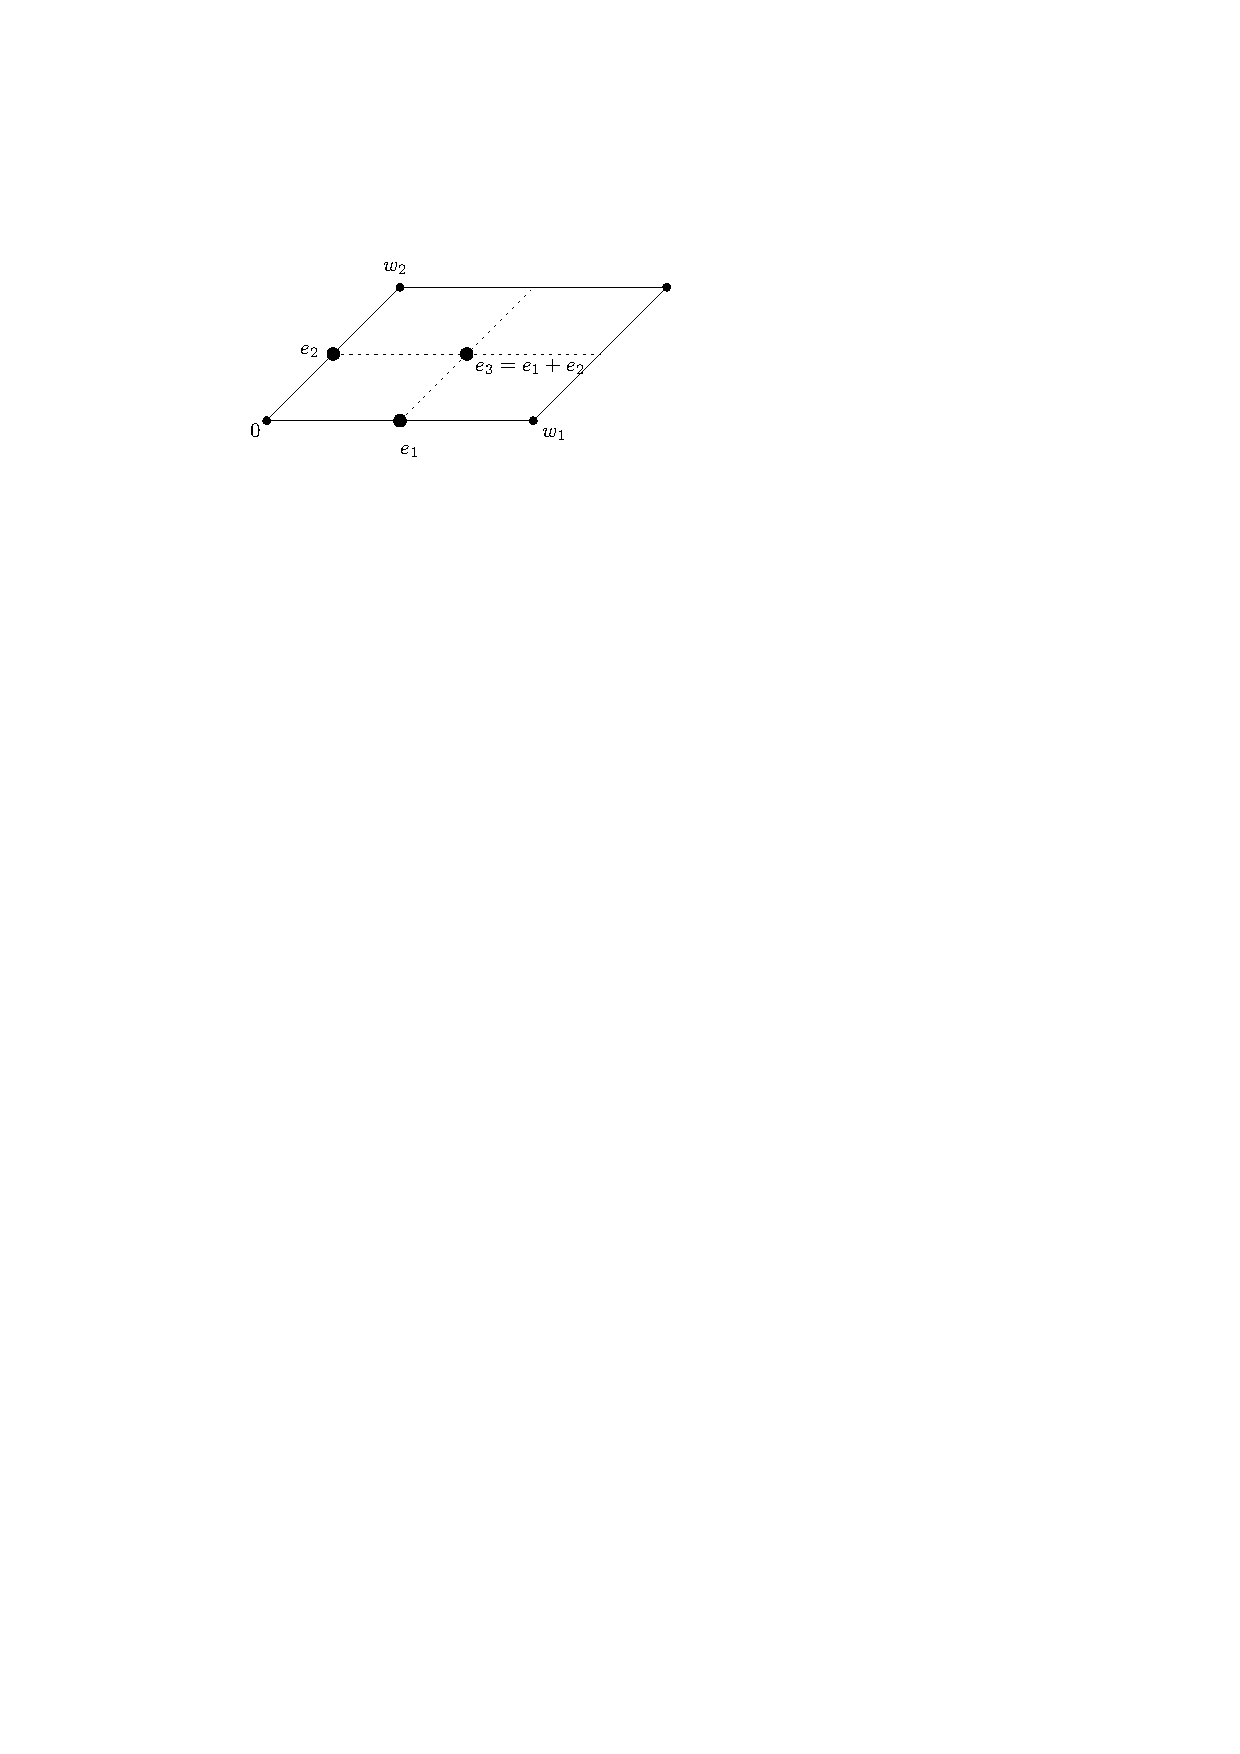
\includegraphics[height=2cm]{twotorsion.pdf}
  \caption{The $2$-torsion points of $E_\Lambda$}
  \label{fig:two-torsion}
\end{figure}

To summarize, what we have found is that there is a holomorphic map:
\[
\CC/\Lambda\to E_\Lambda,\quad z+\Lambda\mapsto (\wp_\Lambda(z),\wp_\Lambda'(z)),
\]
and this map is indeed a bijection: if $x\in\CC$ is any complex number, then $\wp_\Lambda$ takes the value $x$ twice, since $\wp_\Lambda(\pm z+\Lambda)=x$. Therefore we get two $y$-values unless $y=0$ (which happens only when $z=w_i/2$). In this case, $\wp_\Lambda(z)=e_i$, and $\wp_\Lambda(z)$ takes the value $e_i$ ``twice'' at $z$.

The following result is crucial:
\begin{theorem}[Uniformization theorem]
  If $E\colon Y^2=4X^3-g_2X-g_3$ is any elliptic curve, then there exists some lattice $\Lambda$ such that $g_2(\Lambda)=g_2$ and $g_4(\Lambda)=g_4$.
\end{theorem}
\begin{proof}
It uses that $j(z)$ is surjective. See~\cite[Proposition 1.4.3]{diamond-shurman}
\end{proof}
\begin{remark}
  \begin{enumerate}
  \item For $\tau\in\HH$, consider the elliptic curve $E_\tau=E_{\Lambda_\tau}$.
\[
E_\tau\colon Y^2=4X^3-g_2(\tau)X-g_3(\tau).
\]
One can compute that the discriminant of the cubic polynomial on $X$ that is the right-hand side is
\[
\tilde\Delta(\tau) = \frac{1}{16}(g_2(\tau)^3-27g_3(\tau)^2),
\]
which equals $\frac{(2\pi)^{12}}{16}\Delta(\tau)$,
where $\Delta(\tau)$ is the modular form already studied in Section~\ref{sec:a-product-formula-for-Delta}.
\item The map $\CC/\Lambda\to E_\Lambda$ is a group homomorphism. Or if we prefer, we may define the group structure on $E_\Lambda$ via transport of structure.
  \end{enumerate}
\end{remark}

\subsection{Moduli space interpretation}

Consider the set $S$ of isomorphism classes of elliptic curves. Every elliptic curve is isomorphic to $\CC/\Lambda$ for some lattice $\Lambda$, and in fact it is isomorphic to $\CC/\Lambda_\tau$ for some $\tau\in\HH$. Moreover,
\[
\CC/\Lambda_\tau\cong \CC/\Lambda_{\tau'}\iff \SL_2(\ZZ)\tau = \SL_2(\ZZ)\tau'.
\]
Therefore there is a natural bijection
\[
S\longleftrightarrow \SL_2(\ZZ)\backslash \HH,\quad [\CC/\Lambda_\tau]\mapsto \SL_2(\ZZ)\tau.
\]
The quotient $\SL_2(\ZZ)\backslash\HH$ is called the \emphh{moduli space} for isomorphism classes of elliptic curves.

Let now $f\in M_k(\SL_2(\ZZ))$ be a modular form of weight $k$. Define the following function $F$ on the set of complex tori:
\[
F(\CC/\Lambda_\tau) = f(\tau).
\]
This is well defined, because if $\Lambda_\tau=\Lambda_{\tau'}$ then $\tau=\tau'+b$ for some $b\in\ZZ$, and $f(\tau+b)=f(\tau)$. Moreover, suppose that $m\Lambda_\tau=\Lambda_{\tau'}$. Then
\[
\tau=\mtx abcd \tau',\quad m=c\tau'+d.
\]
Then we may compute:
\[
F(\CC/m\Lambda_\tau)=F(\CC/\Lambda_{\tau'}) = f(\tau')=(c\tau'+d)^{-k}f(\tau)=F(\CC/\Lambda_\tau)m^{-k}.
\]
From this we deduce that
\[
F(\CC/m\Lambda) = m^{-k}F(\CC/\Lambda).
\]
We could thus define modular forms as functions on complex tori satisfying the above relations. This prototype can be pushed to work for other congruence subgroups, although isomorphism classes of elliptic curves will have to be replaced by objects carrying more data.

\section{Moduli interpretation for \texorpdfstring{$\Gamma_0(N)$}{Gamma0(N)} and \texorpdfstring{$\Gamma_1(N)$}{Gamma1(N)}}
We will write $E[N]$ for the $N$-torsion in $E=\CC/\Lambda$, which is isomorphic to  $\ZZ/N\ZZ\times \ZZ/N\ZZ$.
\begin{figure}[h]
  \centering
  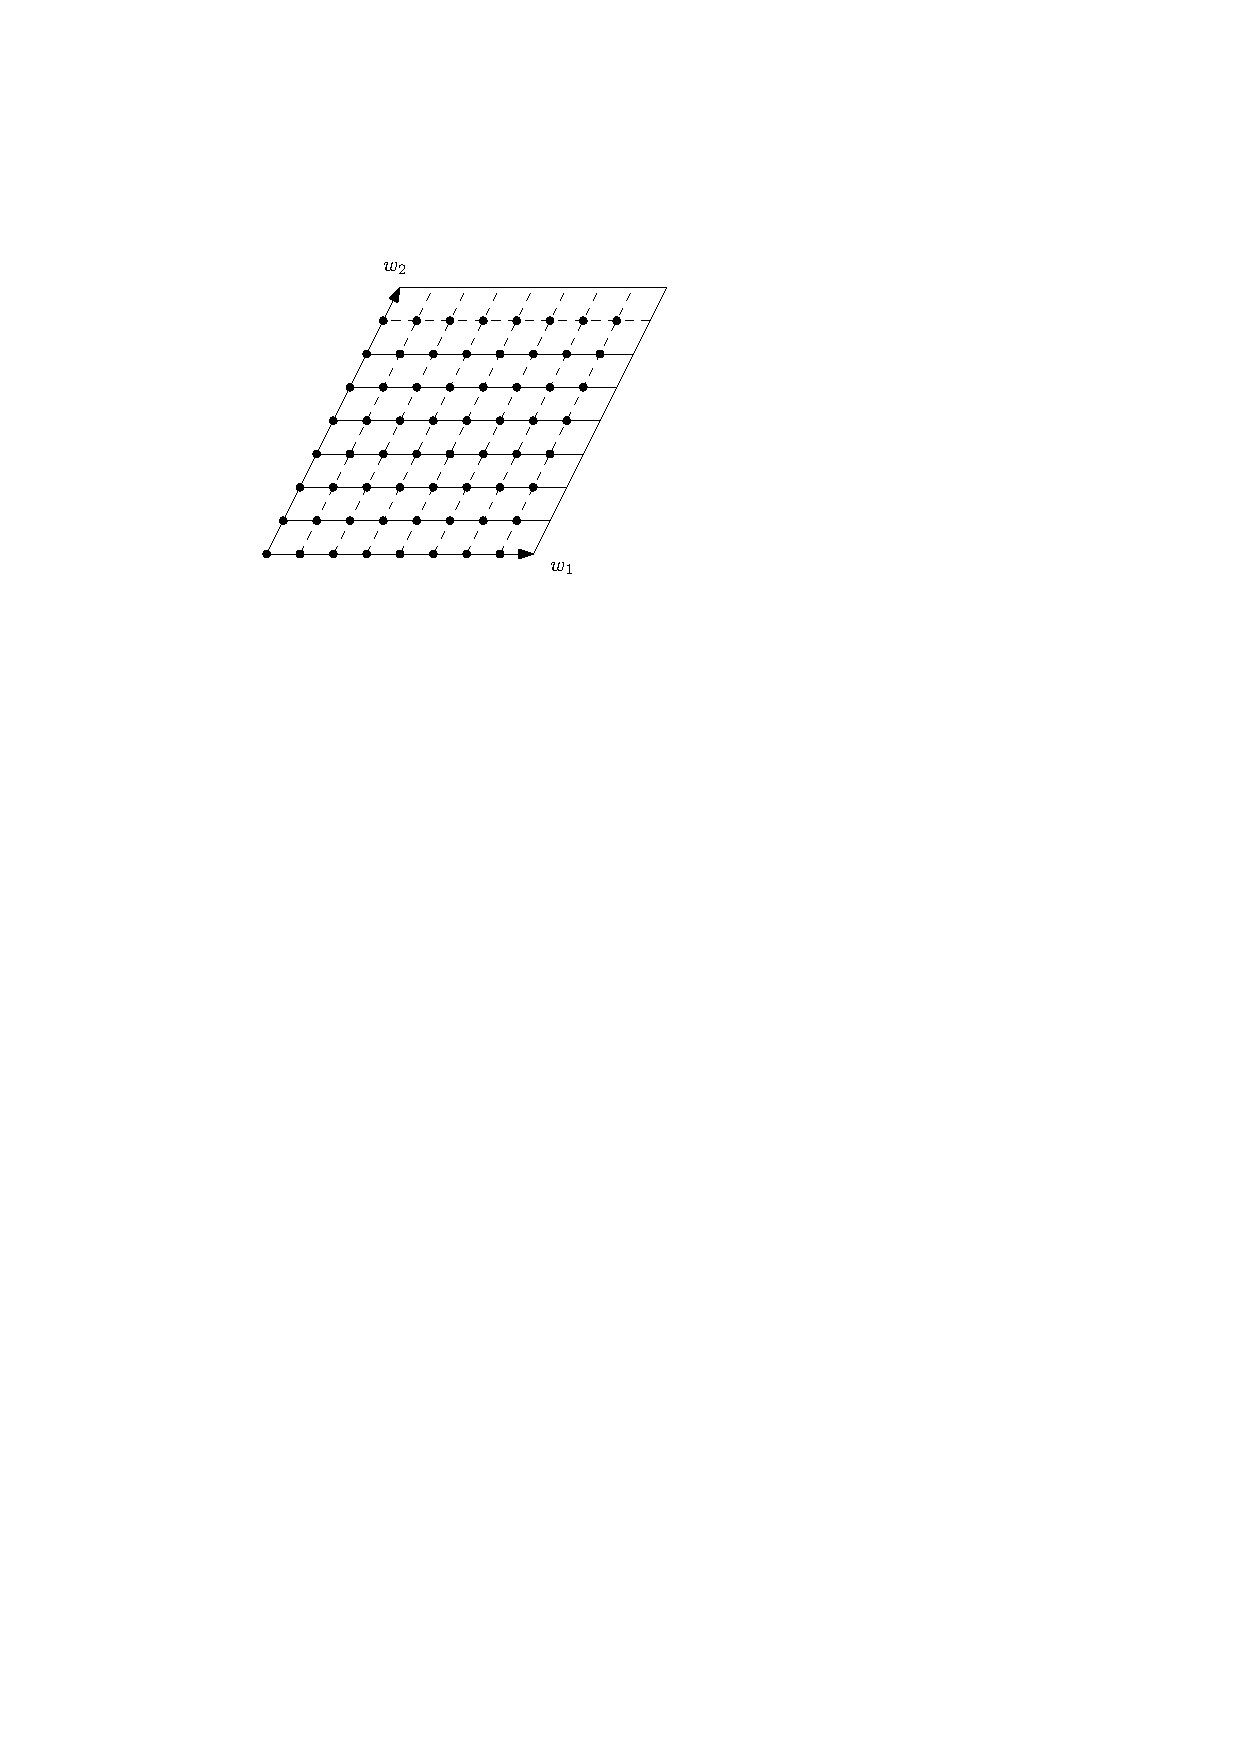
\includegraphics{ntorsion.pdf}
  \caption{The $8$-torsion of a complex torus $\CC/(\ZZ w_1 + \ZZ w_2)$.}
  \label{fig:n-torsion}
\end{figure}
In order to give a moduli interpretation for modular forms on $\Gamma_0(N)$, we need to add more structure
to the elliptic curves (or complex tori) that we consider.
\begin{definition}
  An \emphh{enhanced elliptic curve} for $\Gamma_0(N)$ is a pair $(E,C)$, where $E$ is an elliptic curve
and $C$ is a cyclic subgroup of order $N$ in $E[N]$. Two enhanced elliptic curves $(E,C)$ and $(E',C')$ are
equivalent if there exists an isomorphism $\varphi\colon E\tto{\simeq} E'$ such that $\varphi(C)=C'$.
\end{definition}
We write $S_0(N)$ for the set of equivalence classes of enhanced elliptic curves.

\begin{theorem}
  With the above notation,
  \begin{enumerate}
  \item Each class in $S_0(N)$ has a representative of the form $(\CC/\Lambda_\tau,\langle \frac{1}{N} + \Lambda_\tau\rangle)$, for some $\tau\in\HH$.
  \item Two pairs $(\CC/\Lambda_\tau,\langle \frac{1}{N}+\Lambda_\tau\rangle)$ and $(\CC/\Lambda_{\tau'},\langle \frac{1}{N}+\Lambda_{\tau'}\rangle)$ are equivalent if and only
if $\Gamma_0(N)\tau=\Gamma_0(N)\tau'$. Therefore the map $\tau\mapsto (\CC/\Lambda_\tau,\langle \frac 1N+\Lambda_\tau\rangle)$ induces a bijection of $Y_0(N)=\Gamma_0(N)\backslash\HH\cong S_0(N)$.
  \end{enumerate}
\end{theorem}

\begin{proof}
  Consider an enhanced elliptic curve $(\CC/\Lambda,C)$. We have already seen that there is an isomorphism $\varphi\colon\CC/\Lambda\cong \CC/\Lambda_{\tau'}$ for some $\tau'\in\HH$.
Since $C$ is cyclic of order $N$, the same is true for $\varphi(C)$. Therefore $(\CC/\Lambda,C)$ is equivalent to $(\CC/\Lambda_{\tau'},\langle\frac{c\tau'+d}{N}+\Lambda_{\tau'}\rangle)$ for some integers $c$ and $d$ coprime to each other
and to $N$. Since reduction modulo $N$ gives a surjection $\SL_2(\ZZ)\surjects \SL_2(\ZZ/N/ZZ)$, one can find a matrix
\[
\gamma=\mtx{a'}{b'}{c'}{d'}\in\SL_2(\ZZ),
\]
such that $c'\equiv c\pmod{N}$ and $d'\equiv d\pmod{N}$. Set now $\tau=\gamma\tau'$ and $m=c'\tau'+d'$, so $m\Lambda_\tau=\Lambda_{\tau'}$ and, as we wanted to show,
\[
m\left(\frac 1N + \Lambda_\tau\right)=\frac{c'\tau'+d'}{N}+\Lambda_{\tau'} = \frac{c\tau'+d}{N}+\Lambda_{\tau'},.
\]


As for the second part, for an isomorphism between $\CC/\Lambda_{\tau}$ and $\CC/\Lambda_{\tau'}$ to exist there needs to exist $\gamma=\smtx abcd\in\SL_2(\ZZ)$ such that
\[
(c\tau'+d)\Lambda_\tau = \Lambda_{\tau'}.
\]
Moreover, for the corresponding isomorphism to respect the cyclic subgroups one needs to have
\[
\langle(c\tau'+d)(\frac 1N+\Lambda_\tau)\rangle =\langle \frac 1N+\Lambda_{\tau'}\rangle.
\]
That is, $\gamma$ satisfies
\[
\langle\frac{c\tau'+d}{N}+\Lambda_{\tau'}\rangle = \langle\frac 1N+\Lambda_{\tau'}\rangle,
\]
which is equivalent to $N\mid c$ (and then $d$ is necessarily coprime to $N$). This last condition is precisely saying that $\gamma$ must belong to $\Gamma_0(N)$.
\end{proof}

In this context, one may define a weight-$k$ homogeneous function $F$ for $\Gamma_0(N)$ as a function on enhanced elliptic curves for $\Gamma_0(N)$ such that
\[
F((\CC/m\Lambda,mC) = m^{-k}F(\CC/\Lambda,C),\quad \forall m\in\CC.
\]
Given such an $F$, one can define $f(\tau)=F(\CC/\Lambda_\tau,\langle \frac 1N+\Lambda_\tau\rangle)$ and check that $f(\tau)$ is weakly modular of weight $k$ for $\Gamma_0(N)$.

We have a similar construction for $\Gamma_1(N)$.
\begin{definition}
  An \emphh{enhanced elliptic curve} for $\Gamma_1(N)$ is a pair $(E,P)$, where $E$ is an elliptic curve
and $P$ is a point of exact order $N$ in $E[N]$. Two enhanced elliptic curves $(E,P)$ and $(E',P')$ are
equivalent if there exists an isomorphism $\varphi\colon E\tto{\simeq} E'$ such that $\varphi(P)=P'$.
\end{definition}
We write $S_1(N)$ for the set of equivalence classes of enhanced elliptic curves for $\Gamma_1(N)$.

\begin{theorem}
  With the above notation,
  \begin{enumerate}
  \item Each class in $S_1(N)$ has a representative of the form $(\CC/\Lambda_\tau,\frac{1}{N} + \Lambda_\tau)$, for some $\tau\in\HH$.
  \item Two pairs $(\CC/\Lambda_\tau,\frac{1}{N}+\Lambda_\tau)$ and $(\CC/\Lambda_{\tau'}, \frac{1}{N}+\Lambda_{\tau'})$ are equivalent if and only
if $\Gamma_1(N)\tau=\Gamma_1(N)\tau'$. Therefore the map $\tau\mapsto (\CC/\Lambda_\tau, \frac 1N+\Lambda_\tau)$ induces a bijection of $Y_1(N)=\Gamma_1(N)\backslash\HH\cong S_1(N)$.
  \end{enumerate}
\end{theorem}
\begin{proof}
  Let $(E,Q)$ be any point in $S_1(N)$. Since $E$ is isomorphic to $\CC/\Lambda_{\tau'}$ for some $\tau'\in\HH$, we may take $E=\CC/\Lambda_{\tau'}$, and hence $Q=(c\tau'+d)/N + \Lambda_{\tau'}$ for some $c,d\in\ZZ$. The fact that the order of $Q$ is exactly $N$ means that $\gcd(c,d,N)=1$, and therefore there exists $a,b,k\in\ZZ$ such that
\[
ad-bc-kN=1.
\]
Note that this means that the matrix $\smtx abcd$ has determinant $1\pmod N$. Using that $\SL_2(\ZZ)$ surjects into $\SL_2(\ZZ/N\ZZ)$ and the fact that $c$ and $d$ only matter modulo $N$, we find a matrix $\gamma\in\SL_2(\ZZ)$ with lower low $(c,d)$. Let $\tau=\gamma\tau'$, and let $m=c\tau'+d$. Then we obtain $m\tau=a\tau'+b$, which implies that $m\Lambda_\tau = \Lambda_{\tau'}$. Moreover,
\[
m\left(1/N+\Lambda_\tau\right) = \frac{c\tau'+d}{N}+\Lambda_{\tau'} = Q.
\]
Therefore the class $[E,Q]$ is the same as $[\CC/\Lambda_\tau,1/N+\Lambda_\tau]$.

Finally, given two points $\tau,\tau'\in\HH$ such that $\Gamma_1(N)\tau=\Gamma_1(N)\tau'$, we may write $\tau=\gamma\tau'$ for some $\gamma=\smtx abcd\in\Gamma_1(N)$. Letting $m=c\tau'+d$, then:
\[
m\Lambda_\tau=\Lambda_{\tau'},\quad m\left(1/N+\Lambda_\tau\right)=\frac{c\tau'+d}{N}+\Lambda_{\tau'}.
\]
Since $(c,d)\equiv(0,1)\pmod N$, the last term is just $1/N+\Lambda_{\tau'}$, as we wanted to show.
\end{proof}
Moreover, note that there is a natural map $S_1(N)\to S_0(N)$, which sends the class of $(E,P)$ to that of $(E,\langle P\rangle)$.

There is a moduli space description of $\Gamma(N)\backslash\HH$ which classifies pairs of an elliptic curve $E$ with a \emph{basis} for $E[N]$, but its precise description requires the Weil pairing, which we have not seen in this course.

%%% Local Variables: 
%%% mode: latex
%%% TeX-master: "main"
%%% End: 


\chapter{Hecke Theory}
\label{chap:hecke}
% Hecke Theory
\section{Double coset operators}
Let $\Gamma_1$ and $\Gamma_2$ be two congruence subgroups, and let $\alpha\in\GL_2^+(\QQ)$.
\begin{definition}
  The \emphh{double coset} $\Gamma_1\alpha\Gamma_2$ is the set
\[
\Gamma_1\alpha\Gamma_2=\{\gamma_1\alpha\gamma_2 ~|~ \gamma_1\in\Gamma_1,\gamma_2\in\Gamma_2\}.
\]
\end{definition}
Multiplication gives a left action of $\Gamma_1$ on $\Gamma_1\alpha\Gamma_2$ and another right action of $\Gamma_2$. Consider a decomposition of this double coset into (disjoint) orbits:
\[
\Gamma_1\alpha\Gamma_2=\cup \Gamma_1 \beta_j.
\]
\begin{lemma}
  \begin{enumerate}
  \item If $\Gamma$ is a congruence subgroup and $\alpha\in\GL_2^+(\QQ)$, then $\alpha^{-1}\Gamma\alpha\cap \SL_2(\ZZ)$ is also congruence subgroup.
  \item Any two congruence subgroups $\Gamma_1$, $\Gamma_2$ are \emphh{commensurable}. That is,
\[
[\Gamma_1\colon \Gamma_1\cap\Gamma_2]<\infty\quad\text{ and }\quad [\Gamma_2\colon \Gamma_1\cap\Gamma_2]<\infty.
\]
  \end{enumerate}
\end{lemma}
\begin{proof}
  Let $N$ be a positive integer such that $\Gamma(N)\subseteq \Gamma$, $N\alpha\in M_2(\ZZ)$ and $N\alpha^{-1}\in M_2(\ZZ)$. Set $M=N^3$. Then one can check that $\alpha\Gamma(M)\alpha^{-1} \subseteq \Gamma(N)$,
which implies that $\Gamma(M)\subseteq \alpha^{-1}\Gamma\alpha$. Since $\Gamma(M)$ is also contained in $\SL_2(\ZZ)$, we are done with the first statement.

For the second assertion, just note that there is some $M$ such that $\Gamma(M)\subseteq \Gamma_1\cap\Gamma_2$. Therefore the indices to compute are bounded above by $[\SL_2(\ZZ)\colon\Gamma(M)]$, which is finite.
\end{proof}

\begin{proposition}
  Let $\Gamma_1$ and $\Gamma_2$ be two congruence subgroups, and let $\alpha\in\GL_2^+(\QQ)$. Set $\Gamma_3$ to be the congruence subgroup:
\[
\Gamma_3 = (\alpha^{-1}\Gamma_1\alpha)\cap \Gamma_2.
\]
The map $\gamma_2\mapsto \Gamma_1\alpha\gamma_2$ induces a bijection
\[
\Gamma_3\backslash \Gamma_2 \cong \Gamma_1\backslash \Gamma_1\alpha\Gamma_2.
\]
\end{proposition}
\begin{proof}
  Consider the map
\[
\Gamma_2\to\Gamma_1\backslash (\Gamma_1\alpha\Gamma_2),\quad \gamma_2\mapsto \Gamma_1\alpha\gamma_2.
\]
It is clearly surjective. Moreover, two elements $\gamma_2$ and $\gamma_2'$ get mapped to the same orbit if and only if:
\[
\Gamma_1\alpha\gamma_2=\Gamma_1\alpha\gamma_2'\iff \gamma_2'\gamma_2^{-1}\in\alpha^{-1}\Gamma_1\alpha,
\]
and the latter happens if and only if $\gamma_2$ and $\gamma_2'$ are in the same coset for $(\alpha^{-1}\Gamma_1\alpha) \cap\Gamma_2=\Gamma_3$.
\end{proof}
\begin{corollary}
  Let $\Gamma_2=\cup \Gamma_3\gamma_j$ be a coset decomposition of $\Gamma_3\backslash\Gamma_2$. Then
\[
\Gamma_1\alpha\Gamma_2=\cup \Gamma_1\alpha\gamma_j
\]
is an orbit decomposition. In particular, the number of orbits of $\Gamma_1\alpha\Gamma_2$ under the action of $\Gamma_1$ is finite.
\end{corollary}

  Let $f\in M_k(\Gamma_1)$ be a modular form of weight $k$ for a congruence subgroup $\Gamma_1$. Let $\Gamma_1\alpha\Gamma_2$ be a double coset, where $\Gamma_2$ is a congruence subgroup and $\alpha\in\GL_2^+(\QQ)$. The \emphh{action of the double coset} on $f$ is defined as:
\[
f|_k (\Gamma_1\alpha\Gamma_2) = \sum f|_k \beta_j,
\]
if $\Gamma_1\alpha\Gamma_2=\cup \Gamma_1\beta_j$ is any orbit decomposition.

\begin{remark}
  The action is well defined, independent of the choice of the $\beta_j$. This is so because $f$ is $k$-invariant under $\Gamma_1$.
\end{remark}
The next goal is to show that the double coset operator maps $M_k(\Gamma_1)$ to $M_k(\Gamma_2)$ and preserves cusps forms. We will need a technical lemma to treat the cusp conditions.
\begin{lemma}
\label{lemma:cusp-conditions}
Suppose that for all $\gamma\in\SL_2(\ZZ)$ the function $f|_k\gamma$ has an expansion of the form
\[
\sum_{n\geq n_0} a(n)q_N^n,
\]
with $n_0$ and $a(n)$ depending on $\gamma$. Let $\alpha\in\GL_2^+(\QQ)$. Then for all $\gamma\in\SL_2(\ZZ)$ the function $f|_k(\alpha\gamma)$ has the expansion
\[
\sum_{n\geq an_0} b(n)q_{Nd}^n,
\]
where $a$ and $d$ are positive integers depending only on $\alpha$.
\end{lemma}
\begin{proof}
  First, note that, for $a>0$,
\[
f|_k\mtx a00a = a^{2(k-1)}a^{-k}f = a^{k-2}f.
\]
So without loss of generality we may assume that $\alpha\in M_2(\ZZ)$. Let $\gamma_0\in\SL_2(\ZZ)$ be such that $\gamma_0^{-1}\alpha=\smtx ab0d$ (upper-triangular), with $a$ and $d$ being positive integers. Then:
\begin{align*}
f|_k\alpha &= (f|_k\gamma_0)|_k\mtx ab0d = \left(\sum_{n\geq n_0}a(n)e^{\frac{2\pi i n z}{N}}\right)|_k\mtx ab0d\\
&=(\cdots)\sum_{n\geq n_0} a(n)e^{\frac{2\pi i n(az+b)}{dN}} = (\cdots) q_{Nd}^{an_0}+\cdots
\end{align*}
This concludes the proof.
\end{proof}

\begin{proposition}
\label{prop:double-coset-operators}
Let $\Gamma_1$ and $\Gamma_2$ be two congruence subgroups, and let $\alpha\in\GL_2^+(\QQ)$.
The rule $f\mapsto f|_k\Gamma_1\alpha\Gamma_2$ induces a map $M_k(\Gamma_1)\to M_k(\Gamma_2)$.
\end{proposition}
\begin{proof}
 Write $\Gamma_3=(\alpha^{-1}\Gamma_1\alpha)\cap \Gamma_2$, and consider a coset decomposition $\Gamma_2= \cup \Gamma_3\gamma_j$. One can take as set of representatives $\beta_j=\alpha\gamma_j$. If $\gamma_2\in\Gamma_2$, then $\{\gamma_j\gamma_2\}_j$ is a complete set of representatives for $\Gamma_3\backslash \Gamma_2$, and hence $\{\alpha\gamma_j\gamma_2\}_j$ is a complete set of representatives for $\Gamma_1\backslash\Gamma_1\alpha\Gamma_2$. This implies that $f|_k\Gamma_1\alpha\Gamma_2$ is $k$-invariant for $\Gamma_2$.

If $f$ is holomorphic on $\HH$, then $f|_k\beta_j$ is holomorphic on $\HH$ for any $\beta_j\in\GL_2^+(\QQ)$, so it only remains to check the cusp conditions. But Lemma~\ref{lemma:cusp-conditions} precisely ensures that these are preserved.
\end{proof}

\subsection{First examples}
Consider the case $\Gamma_2\subseteq \Gamma_1$ and $\alpha=1$. Then $\Gamma_1\alpha\Gamma_2=\Gamma_1$, and $\Gamma_1=\Gamma_11$ is an orbit decomposition. Therefore $f|_k\Gamma_1\alpha\Gamma_2 = f|_k1 = f$. This just says that $M_k(\Gamma_1)$ is a subspace of $M_k(\Gamma_2)$.

As a more interesting example, given $\alpha\in\GL_2^+(\QQ)$ consider the conjugate $\Gamma'=\alpha^{-1}\Gamma\alpha$. Then $\Gamma\alpha\Gamma'=\Gamma\alpha$ is an orbit decomposition. This implies that acting by $\alpha$ induces a map
\[
M_k(\Gamma)\to M_k(\alpha^{-1}\Gamma\alpha).
\]
Since the inverse of this map is given by the action of $\alpha^{-1}$, we conclude that $M_k(\Gamma)$ and $M_k(\alpha^{-1}\Gamma\alpha)$ are naturally isomorphic.

Finally, consider the case $\Gamma_1\subseteq \Gamma_2$ and $\alpha=1$. Then $\Gamma_1\alpha\Gamma_2 = \cup \Gamma_1 \beta_j$, where $\beta_j$  is a set of coset representatives for $\Gamma_1\backslash \Gamma_2$. The map
\[
f\mapsto \sum_{j} f|_k \beta_j
\]
is to be seen as a \emph{trace operator} from $M_k(\Gamma_1)\to M_k(\Gamma_2)$. In particular, it maps $f\in M_k(\Gamma_2)$ to $[\Gamma_2\colon \Gamma_1]f$ and thus it is surjective.

\section{Hecke operators for \texorpdfstring{$\Gamma_1(N)$}{Gamma1(N)}}
Fix now $\Gamma=\Gamma_1(N)$. We will describe the Hecke operators for the group $\Gamma$.

\subsection{The \texorpdfstring{$T_p$}{Tp} operators}
Let $p$ be a prime. The \emphh{Hecke operator} at $p$ is defined as:
\[
T_p f = f|_k\Gamma_1(N)\mtx{1}{0}{0}{p}\Gamma_1(N).
\]
By Proposition~\ref{prop:double-coset-operators}, the operator $T_p$ acts on $M_k(\Gamma_1(N))$.

In order to describe the action of $T_p$ more precisely, we need to understand the double coset $\Gamma_1(N)\smtx 100p\Gamma_1(N)$. Note first that if $\gamma\in \Gamma_1(N)\smtx 100p\Gamma_1(N)$ then:
\begin{enumerate}
\item $\det \gamma = p$, and
\item $\gamma\equiv\smtx 1{*}0p\pmod N$.
\end{enumerate}
In fact, the converse is true:
\begin{lemma}
  We have that
\[
\Gamma_1(N)\mtx{1}{0}{0}{p}\Gamma_1(N)=\left\{\gamma\in M_2(\ZZ)~|~\det\gamma = p,\gamma\equiv \smtx{1}{*}{0}{p}\pmod{N}\right\}.
\]
\end{lemma}
\begin{proof}
To prove the remaining inclusion, let $\gamma\in M_2(\ZZ)$ have determinant $p$, and satisfy  $\gamma\equiv \smtx 1{*}0p\pmod N$. Consider $L=\ZZ^2$ and
\[
L_0=L_0(N)=\{\smat{x\\y}\in L\colon y\equiv 0\pmod N\}.
\]
Note that $\gamma L_0\subseteq L_0$. Since $\det \gamma=p>0$, we have:
\[
[L\colon\gamma L_0]=[L\colon L_0][L_0\colon\gamma L_0] = Np.
\]
Choose a basis of $L$ adapted to $\gamma L_0$. That is, a basis $u$, $v$ such that $\det(u|v)=1$ and such that
\[
\gamma L_0=mu\ZZ\oplus nv\ZZ, \text{ with } 0<m\mid n, mn=Np.
\]
We will show:
\begin{enumerate}
\item $\gamma L_0=u\ZZ\oplus Np v\ZZ$.
\item $L_0 = u\ZZ\oplus Nv\ZZ$.
\item $\gamma L = u\ZZ+pv\ZZ$.
\end{enumerate}
In fact, since $\gamma\smat{1\\0}\in \gamma L_0$, we have that $\smat{a\\b}\equiv\smat{0\\0}\pmod m$. Since $\gcd(a,N)=1$, this implies that $\gcd(m,N)=1$. Now, if $p\mid m$, then $p\mid n$, and so $p^2\mid mn=Np$. Therefore $p\mid N$, which is a contradiction with $\gcd(m,N)=1$. Therefore $p\nmid m$ and hence $m=1$ and $n=Np$.

The two other facts follow because $L_0\subset L$ is a subgroup of index $N$, and $\gamma L\subset L$ is of index $p$ in $L$. This proves the above three statements.

Next,  set $\gamma_1=(u|v)$, which belongs to $\Gamma_0(N)$ because $u$ belongs to $L_0$. Set also $\gamma_2=(\gamma_1\smtx 100p)^{-1}\gamma$, so that $\gamma=\gamma_1\smtx 100p\gamma_2$. Note that $\gamma_2$ belongs to $\SL_2(\QQ)$. It remains to show that $\gamma_1$ and $\gamma_2$ belong to $\Gamma_1(N)$. This will follow if we can prove:
\begin{enumerate}
\item $\gamma_2\in \Gamma_0(N)$.
\item $\Gamma_0(N)\smtx 100p \Gamma_0(N)=\Gamma_1(N)\smtx 100p\Gamma_0(N)$.
\item If $\gamma=\gamma_1\smtx 100p\gamma_2$ with $\gamma_1\in \Gamma_1(N)$ and $\gamma_2\in \Gamma_0(N)$, then $\gamma_2$ belongs to $\Gamma_1(N)$.
\end{enumerate}
Each of these statements can be easily proved, and we ommit these proofs.
\end{proof}

\begin{proposition}
\label{prop:description-hecke}
  Let $f\in M_k(\Gamma_1(N))$. Then $T_p f$ is given by:
\[
T_p f =
\begin{cases}
\sum_{j=0}^{p-1} f|_k \mtx 1j0p&p\mid N,\\
\sum_{j=0}^{p-1} f|_k\mtx 1j0p +f|_k\mtx{mp}{n}{Np}{p}&p\nmid N.
\end{cases}
\]
Here the matrix $\smtx{mp}{n}{Np}{p}$ is chosen such that $\gamma_\infty=\smtx{mp}{n}{N}{1}$ belongs to $\Gamma_1(N)$.
\end{proposition}
\begin{proof}
  We just need to trace the definition of the double coset operator. That is, we need to find an explicit coset decomposition of $\Gamma_3\backslash \Gamma_1(N)$, where
\[
\Gamma_3={\mtx 1 0 0 p}^{-1} \Gamma_1(N) \mtx 100p \cap \Gamma_1(N).
\]
Define $\Gamma^0(p)$ to be the group of matrices which are lower triangular modulo $p$. It is easy to see that
\[
\Gamma_3 = \Gamma_1(N)\cap \Gamma^0(p).
\]
Consider the matrices $\gamma_j=\smtx 1j01$, with $j$ ranging from $0$ to $p-1$ inclusive. These are all distinct modulo $\Gamma_1(N)\cap \Gamma^0(p)$ (check it). Given any matrix $\smtx abcd \in\Gamma_1(N)$, note that
\[
\mtx abcd \mtx 1{-j}01 = \mtx{a}{-aj+b}{c}{-cj+d}.
\]
Therefore if $p\nmid a$ we can make the right-hand side to belong to $\Gamma^0(p)$ for some $j$. This means that if $p$ divides $N$ then $p$ will not divide $a$ (because of the determinant condition), and thus the set $\{\gamma_j\}$ is a complete set of representatives. If $p\nmid N$, we need to consider matrices $\smtx abcd$ with $p\mid a$. Choose some $\gamma_\infty=\smtx{mp}{n}{N}{1}\in\Gamma_1(N)$. Then:
\[
\mtx abcd \gamma_\infty^{-1} = \mtx{*}{-na+bmp}{0}{*}.
\]
Since $p$ divides $-na+bmp$, the matrix $\smtx abcd$ is in the coset of $\gamma_\infty$ modulo $\Gamma^0(p)$. Hence $\{\gamma_j\}\cup \{\gamma_\infty\}$ forms a complete set of representatives. In order to get the orbit representatives for the double coset, we just need to multiply the $\gamma_j$ by the fixed element $\alpha = \smtx 100p$.
\end{proof}

\subsection{The diamond \texorpdfstring{$\langle d \rangle$}{d} operators}

We define another (finite) set of operators on $M_k(\Gamma_1(N))$, called the diamond operators. First we need some preliminaries on characters.
\begin{definition}
  A \emphh{Dirichlet character} modulo $N$ is a group homomorphism
\[
\chi\colon (\ZZ/N\ZZ)^\times\to\CC^\times.
\]
\end{definition}
It can be extended to a map $\chi\colon \ZZ\to \CC$ by the recipe
\[
\chi(d) = \begin{cases}
\chi(d\bmod N)&(d,N)=1\\
0&(d,N)\neq 1.
\end{cases}
\]
The resulting function is totally multiplicative: it satisfies
\[
\chi(d_1d_2)=\chi(d_1)\chi(d_2)\quad \forall d_1,d_2\in\ZZ.
\]
Consider the map $\Gamma_0(N)\to\ZZ/N\ZZ^\times$ sending a matrix $\smtx abcd$ to $d\bmod N$. Its kernel is precisely $\Gamma_1(N)$, and therefore we obtain an isomorphism
\[
\Gamma_0(N)/\Gamma_1(N)\cong (\ZZ/NZ)^\times,\quad \mtx abcd \Gamma_1(N)\mapsto d\bmod N.
\]

\begin{definition}
Given $d\in \ZZ$ coprime to $N$, the \emphh{diamond operator} $\langle d\rangle$ is the operator on $M_k(\Gamma_1(N))$ defined as
\[
\langle d \rangle f = f|_k \mtx abc{d'},
\]
where $a$, $b$, $c$, $d'$ are chosen so that $\smtx abc{d'}$ belongs to $\Gamma_0(N)$ and $d'\equiv d\pmod N$. 
\end{definition}
Note that the above is well defined, and only depends on the class of $d$ modulo $N$. This is precisely because $\Gamma_0(N)/\Gamma_1(N)\cong (\ZZ/NZ)^\times$. The operator $\langle d\rangle$ is a linear invertible map, and thus it makes sense to look at its eigenspaces.

\begin{definition}
  The \emph{space of modular forms with character} $\chi$ is
\[
M_k(\Gamma_0(N),\chi)=\{f\in M_k(\Gamma_1(N))~|~ f|_k\smtx abcd = \chi(d) f,\smtx abcd\in \Gamma_0(N)\}.
\]
The \emphh{space of cusp forms with character} $\chi$ is defined similarly and written $S_k(\Gamma_0(N),\chi)$.
\end{definition}

Note that $M_k(\Gamma_0(N),\chi)$ can also be defined as
\[
M_k(\Gamma_0(N),\chi)=\{f\in M_k(\Gamma_1(N))~|~ \langle d\rangle f = \chi(d) f,\quad d\in (\ZZ/N\ZZ)^\times\}.
\]

\begin{theorem}
  There is a decomposition of $\CC$-vector spaces
\[
M_k(\Gamma_1(N))=\bigoplus_{\chi\bmod N} M_k(\Gamma_0(N),\chi),
\]
where the sum runs over the $\phi(N)=\#(\ZZ/N\ZZ)^\times$ Dirichlet characters modulo $N$.
\end{theorem}
\begin{proof}
  Picking a basis of $M_k(\Gamma_1(N))$, we get a representation
\[
\rho\colon (\ZZ/N\ZZ)^\times\to \GL_n(\CC),\quad \rho(d)=\langle d\rangle,
\]
where $n$ is the dimension of $M_k(\Gamma_1(N))$. Since $(\ZZ/N\ZZ)^\times$ is abelian, the representation $\rho$ decomposes as a sum of irreducible representations, which are necessarily one-dimensional. This means that we can pick a basis for $M_k(\Gamma_1(N))$ such that
\[
\rho(d) = \diag(\chi_1(d),\ldots,\chi_n(d)).
\]
This means that $\langle d\rangle$ acts as $\chi_i(d)$ on the $i$th component. One just needs to collect then the repeated $\chi$ to form $M_k(\Gamma_0(N),\chi)$.
\end{proof}

\subsection{Hecke operators on \texorpdfstring{$q$}{q}-expansions}
In order to study the action of Hecke operators on $q$-expansion, we introduce two simple operators: if $f=\sum a_n q^n$, define:
\[
U_p f = \sum a_{np} q^n=\sum a_n q^{n/p}.
\]
The second equality is an abuse of notation: we define $q^{n/p}=0$ if $p\nmid n$. We define also:
\[
V_p f = f(pz) = \sum a_n q^{np} = \sum a_{n/p} q^n.
\]
\begin{lemma}
  If $f=\sum a_n q^n$, then
  \begin{enumerate}
  \item \[
U_p f = \frac 1p \sum_{j=0}^{p-1} f\left(\frac{z+j}{p}\right) = \sum_{j=0}^{p-1} f|_k \mtx 1j0p.
\]

\item \[V_p f= p^{1-k} f|_k\mtx p001. \]
  \end{enumerate}
\end{lemma}
\begin{proof}
  Note that if $\zeta_p=e^{\frac{2\pi i}{p}}$ is a primitive $p$th root of unity, then
\[
\sum_{j=0}^{p-1} \zeta_p^{nj} = \begin{cases}
p&p\mid n\\
0&p\nmid n.
\end{cases}
\]
Now compute:
\[
\sum_{j=0}^{p-1} f|_k \mtx 1j0p = p^{k-1} p^{-k}\sum_j f\left(\frac{z+j}{p}\right).
\]
Since $f$ is $1$-periodic, this is the same as:
\[
\frac 1p \sum_j \sum_n a_n e^{2\pi i \frac{z+j}{p}} = \sum_n a_n e^{\frac{2\pi i n z}{p}} \frac 1p \sum_j \zeta_p^{nj}.
\]
This proves the first statement. The second statement is clear.
\end{proof}

 Putting together what we have seen so far, we get a description of $T_p$ in terms of $U_p$, $V_p$ and the diamond operators.
\begin{theorem}
We have:
\[
T_p f = \begin{cases}
U_p f&p\mid N,\\
U_p f + p^{k-1} V_p\langle p\rangle f&p\nmid N.
\end{cases}
\]
\end{theorem}
\begin{corollary}
  If $f\in M_k(\Gamma_0(N),\chi)$ then for all $p$ we have:
\[
T_p f= U_p f +\chi(p)p^{k-1}V_p f.
\]
In particular, if $f\in M_k(\Gamma_0(N))$ then:
\[
T_p f =
\begin{cases}
  U_p f&p\mid N,\\
U_p f +p^{k-1}V_pf& p\nmid N.
\end{cases}
\]
\end{corollary}
Moreover, the relation between $U_p$ and $T_P$ allows us to think of $U_p$ as an operator on modular forms, which possibly raises the level.
\begin{corollary}
  \begin{enumerate}
  \item   If $p\mid N$ then $U_p$ maps $M_k(\Gamma_1(N))$ to itself.
\item  If $p\nmid N$ then $U_p$ maps $M_k(\Gamma_1(N))$ to $M_k(\Gamma_1(Np))$.
  \end{enumerate}

\end{corollary}

\begin{example}
  Consider the Eisenstein series
\[
E_k(z)=1-\frac{2k}{B_k}\sum_{n=1}^\infty \sigma_{k-1}(n)q^n\in M_k(\Gamma_1(1)).
\]
\begin{proposition}
  \label{prop:Ek-is-eigen}
We have:
\[
T_p E_k = \sigma_{k-1}(p) E_k = (1+p^{k-1})E_k.
\]
That is, $E_k$ is an eigenform for all $T_p$, with eigenvalue $\sigma_{k-1}(p)$.
\end{proposition}
\begin{proof}
 In general we have seen that, since $E_k\in M_k(\Gamma_0(1))$),
\[
a_n(T_pf)= a_n(U_p f) + p^{k-1} a_n(V_p f) = a_{np}(f)+p^{k-1} a_{n/p}(f).
\]
So
\[
a_0(T_pE_k) = a_0(E_k) + p^{k-1} a_0(E_k) = \sigma_{k-1}(p) a_0(E_k).
\]
For $n\geq 1$, we get
\[
a_n(T_pE_k) = \frac{-2k}{B_k}\left(\sigma_{k-1}(np)+p^{k-1}\sigma_{k-1}(n/p)\right),
\]
where we understand that $\sigma_{k-1}(n/p)=0$ if $p\nmid n$. We claim that:
\[
\sigma_{k-1}(pn) + p^{k-1}\sigma_{k-1}(n/p) = \sigma_{k-1}(p)\sigma_{k-1}(n),\quad \forall n\geq 1.
\]
When $p\nmid n$, this is just the multiplicativity of $\sigma_{k-1}$. If $p\mid n$, write $n=p^em$ with $p\nmid m$. Then we need to show that for all $e\geq 1$
\[
\sigma_{k-1}(p^{e+1}m) + p^{k-1}\sigma_{k-1}(p^{e-1}m) = \sigma_{k-1}(p)\sigma_{k-1}(p^em).
\]
This follows easily by dividing both sides by $\sigma_{k-1}(m)$, which is a common factor of both sides of the equation again by multiplicativity of $\sigma_{k-1}$.
\end{proof}
\begin{remark}
  If $f=1+\sum_{n\geq 1} a_n q^n$ is a modular form for $\SL_2(\ZZ)$ of weight $k$ and it is an eigenform for $T_p$, then the eigenvalue must be $\sigma_{k-1}(p)$, by the first calculation of the above proof. The real content of the proposition is thus that $E_k$ is actually an eigenform.
\end{remark}
\end{example}
\section{The Hecke algebra}
\begin{definition}
  Let $N\geq 1$ and $k\in \ZZ$. The \emphh{Hecke algebra} acting on $M_k(\Gamma_1(N))$ is the $\CC$-subalgebra of $\End_\CC M_k(\Gamma_1(N))$ generated by
\[
\Big\langle T_p\colon p\text{ prime};\text{ and } \langle d\rangle \colon d\in (\ZZ/N\ZZ)^\times\Big\rangle.
\]
The Hecke algebra is denoted by $\bbT(M_k(\Gamma_1(N)))$. Similarly we define $\bbT(S_k(\Gamma_1(N)))$ as a subalgebra of $\End_\CC S_k(\Gamma_1(N))$.
\end{definition}

\begin{theorem}
  For every $N\geq 1$ the Hecke algebra $\bbT(M_k(\Gamma_1(N)))$ is commutative.
\end{theorem}
\begin{proof}
We must show that for all primes $p$, $q$ and all elements $e$ and $d$ of $(\ZZ/N\ZZ)^\times$ we have:
  \begin{enumerate}
  \item $\langle d\rangle T_p = T_p \langle d\rangle$,
  \item $\langle d \rangle \langle e\rangle = \langle e\rangle\langle d\rangle$, and
  \item $T_p T_q = T_q T_p$.
  \end{enumerate}

First we show (2) and (3) assuming (1). Note that (1) means that $T_p$ preserves the spaces $M_k(\Gamma_0(N),\chi)$ and so it's enough to check (2) and (3) for forms $f\in M_k(\Gamma_0(N),\chi)$. This makes (2) obvious. As for (3), we can use the $q$-expansions: if $f=\sum a_n q^n$, then
\[
a_n(T_p f)= a_{pn}(f) + \chi(p)p^{k-1} a_{n/p}(f).
\]
Then:
\begin{align*}
a_n(T_pT_qf) &= a_{pn}(T_qf) + \chi(p)p^{k-1}a_{n/p}(T_qf)\\
&=a_{pqn}(f) + \chi(q) q^{k-1} a_{pn/q}(f)+\chi(p)p^{k-1}(a_{nq/p}(f)+\chi(q) q^{k-1} a_{n/(pq)}(f)).
\end{align*}
This formula is symmetric in $p$ and $q$ so we are done.

Finally, to prove (1) we must write $\langle d\rangle$ as a double coset. Let $\gamma\equiv \smtx{*}{*}{0}{d}\pmod N$. Write $\Gamma=\Gamma_1(N)$. Then, since $\Gamma$ is normal in $\Gamma_0(N)$, we have
\[
\Gamma\gamma\Gamma=\Gamma\gamma,
\]
and thus $\langle d\rangle f = f|_k \gamma$. We want to show that $\langle d\rangle^{-1}T_p\langle d\rangle = T_p$. Write $\Gamma\alpha\Gamma=\bigcup_j \Gamma \beta_j$ for the orbit decomposition of the double coset corresponding to $T_p$. We thus need to show that
\[
\Gamma\alpha\Gamma=\bigcup_j \Gamma(\gamma\beta_j\gamma^{-1}).
\]
We note that
\[
\bigcup_j \Gamma (\gamma\beta_j\gamma^{-1}) = \gamma\left(\bigcup_j \Gamma \beta_j\right)\gamma^{-1} = \gamma(\Gamma\alpha\Gamma)\gamma^{-1} = \Gamma(\gamma\alpha\gamma^{-1})\Gamma,
\]
and one just checks then that
\[
\Gamma\alpha\Gamma = \Gamma(\gamma\alpha\gamma^{-1})\Gamma.
\]
\end{proof}

Next, we define operators $T_n$ and $\langle n\rangle$ for all $n\geq 1$. First, define $\langle p\rangle =0$ whenever $p\mid N$. One can implicitly define $T_n$ by the following formula:
\[
\sum_{n=1}^\infty T_n n^{-s} = \prod_p \frac{1}{1-T_pp^{-s} + \langle p\rangle p^{k-1-2s}}.
\]
This in turn is equivalent to the following conditions:
\begin{enumerate}
\item $T_{nm} = T_n T_m$ if $(n,m)=1$,
\item $T_1 = \operatorname{id}$, and
\item for all primes $p$ and for all $r\geq 2$,
\[
T_{p^r} = T_p T_{p^{r-1}} - p^{k-1}\langle p\rangle T_{p^{r-2}}.
\]
\end{enumerate}

From the definition we can see that each $T_n$ is an explicit polynomial on the $T_p$, and therefore all $T_n$ commute with each other.

\begin{theorem}[Action of $T_n$ on $q$-expansions]
  Suppose $f\in M_k(\Gamma_1(N))$ has an expansion of the form $\sum a_m(f)q^m$. Then $T_n(f)=\sum a_m(T_nf) q^m$, where
\[
a_m(T_nf) = \sum_{d\mid (m,n)} d^{k-1}a_{\frac{mn}{d^2}}(\langle d\rangle f).
\]
In particular, if $f\in M_k(\Gamma_0(N),\chi)$ then
\[
a_m(T_nf)=\sum_{d\mid (m,n)} \chi(d) d^{k-1} a_{\frac{mn}{d^2}}(f).
\]
\end{theorem}
\begin{proof}
  A long computation.
\end{proof}

We end this section with the notion of Hecke eigenforms.
\begin{definition}
  A \emphh{Hecke eigenform} (or just eigenform) is a non-zero modular form $f\in M_k(\Gamma_1(N))$ which is an eigenvector for all the Hecke algebra $\bbT(M_k(\Gamma_1(N))$. A \emphh{normalized Hecke eigenform} (or normalized eigenform) is an eigenform satisfying $a_1(f)=1$.
\end{definition}

Let $f\in M_k(\Gamma_1(N))$ be an eigenform, say $T_nf=\lambda_n f$ for all $n$. Then we obtain
\[
a_n(f) = a_1(T_n f) = \lambda_n a_1(f),\quad n\geq 1.
\]
So if $a_1(f)=0$ then all $a_n(f)=0$ and thus $f=0$. Therefore a non-constant non-zero eigenform must have $a_1(f)\neq 0$ and it may be scaled to a normalized eigenform. In particular, we have the following.
\begin{theorem}
  Let $f\in M_k(\Gamma_1(N))$ be a normalized eigenform. Then the eigenvalues of the Hecke operators on $f$ are precisely the coefficients of the $q$-expansion of $f$ at the cusp $\infty$:
\begin{equation}
\label{eq:ans-for-hecke}
T_n f = a_n(f) f,\quad n\geq 1.
\end{equation}
\end{theorem}
\begin{proof}
Write $\lambda_n$ for the eigenvalue of the Hecke operator $T_n$. By Equation~\eqref{eq:ans-for-hecke} we have $a_n(f) = a_1(T_n f) = \lambda_n a_1(f)$. Since $f$ is normalized, $a_1(f)=1$ and hence $a_n(f) = \lambda_n$.
\end{proof}
In fact, the Fourier coefficients of a modular form readily tell whether it is a normalized eigenform:
\begin{proposition}
\label{proposition:coeffsnormalizedeigen}
  Let $f\in M_k(\Gamma_0(N),\chi)$ be a modular form with $q$-expansion $\sum_{n=0}^\infty a_n(f) q^n$. Then $f$ is a normalized eigenform if and only if:
  \begin{enumerate}
  \item $a_1(f) = 1$,
  \item $a_{mn}(f) = a_m(f) a_n(f)$ whenever $(m,n)=1$, and
\item $a_{p^r}(f) = a_p(f)a_{p^{r-1}}(f) - p^{k-1}\chi(p) a_{p^{r-2}}(f),\quad r\geq 2$.
  \end{enumerate}
\end{proposition}
\begin{proof}
  The implication $\implies$ follows directly from the previous proposition and the definition of the Hecke operators $T_n$. For the converse, if $f\in M_k(\Gamma_0(N),\chi)$ satisfies $(1)$, $(2)$ and $(3)$ then $f$ is already normalized, so to be an eigenform we must show that it satisfies
\[
a_m(T_pf)=a_p(f)a_m(f),\quad \forall p\text{ prime}, \forall m\geq 1.
\]
If $p\nmid n$ then it follows from the formula that we have for $T_m$ on $q$-expansions that $a_m(T_pf)=a_{pm}(f)$, which by $(2)$ is $a_p(f)a_m(f)$. If $p\mid m$ then writing $m=p^rm'$ with $r\geq 1$ and $p\nmid m'$ we have by the same formula
\[
a_m(T_pf) = a_{p^{r+1}m'}(f) + \chi(p)p^{k-1}a_{p^{r-1}m'}(f).
\]
Using now conditions $(2)$ and $(3)$ this can be rewritten as $a_p(f)a_m(f)$, as wanted.
\end{proof}
\section{Petersson inner product}
\subsection{Surface integrals}
Let $V\subseteq \CC$. A $2$-form on $V$ is an expression of the form $\omega = f(z,\bar z)dz\wedge d\bar z$. Note that
\[
dz\wedge d\bar z = (dx + i dy)\wedge (dx-idy) = -2idx\wedge dy.
\]
The integral of $\omega$ on $V$ is:
\[
\int_V \omega = \int_V f(z,\bar z dz\wedge d\bar z=\int\int -2i f(x+iy,x-iy)dxdy.
\]
Consider now, for $\alpha\in\GL_2^+(\RR)$, the change $z\mapsto \alpha z$. Then:
\[
\Im(\alpha z)=\frac{\det \alpha}{|cz+d|^2}\Im(z),
\]
and also
\[
d(\alpha z) = \frac{\det \alpha}{(cz+d)^2} dz,\quad \ol{d(\alpha z)} = \frac{\det\alpha}{\ol{(cz+d)^2}} d\bar z.
\]
This gives that:
\[
d(\alpha z)\wedge d\ol{\alpha z} = \frac{(\det \alpha)^2}{|cz + d|^4} dz\wedge d\bar z.
\]
Therefore the $2$-form $\frac{dz\wedge d\bar z}{\Im(z)^2}$ is invariant under changes of the form $z\mapsto \alpha z$. We will work instead with a certain multiple of this $2$-form. Define
\[
d\mu(z) = \frac{dx\wedge dy}{y^2} = \frac{-1}{2i} \frac{dz\wedge d\bar z}{\Im(z)^2}.
\]
We can define the \emphh{covolume} of $\SL_2(\ZZ)$ as
\[
\covol(\SL_2(\ZZ)) = \int_{D^*} d\mu(z).
\]
where $D^*$ is a fundamental domain for $\SL_2(\ZZ)$.
\begin{lemma}
  \[\covol(\SL_2(\ZZ)) = \frac{\pi}{3}.\]
\end{lemma}
\begin{proof}
  Exercise.
\end{proof}
\begin{corollary}
  If $\varphi$ is a bounded function on $D^*$, then $\int_{D^*} \varphi(z)d\mu(z)$ is a well-defined complex number.
\end{corollary}

\subsection{Integral over \texorpdfstring{$X(\Gamma)$}{X(Gamma)}}
Let $\cD$ be a fundamental domain for a congruence subgroup $\Gamma$. Such a fundamental domain is the union (almost disjoint) of translates of $D^*$:
\[
\cD=\cup_j \alpha_j D^*,
\]
where $\{\alpha_j\}$ is a set of coset representatives for $(\pm 1\cdot \Gamma)\backslash \SL_2(\ZZ)$. If $\varphi$ is $\Gamma$-invariant, then we may define the integral of $\varphi$ on $X(\Gamma)=\Gamma\backslash \HH$ as:
\[
\int_{X(\Gamma)} \varphi(\tau) d\mu(\tau) = \sum_j \int_{\alpha_j D^*} \varphi(\tau)d\mu(\tau) = \sum_j\int_{D^*} \varphi(\alpha_j\tau)d\mu(\alpha_j\tau)=\sum_j\int_{D^*} \varphi(\alpha_j\tau)d\mu(\tau).
\]
The last term in the above equality shows that the definition is independent of the choice of coset representatives. We may calculate the covolume of $\Gamma$ as:
\begin{lemma}
\label{lemma:covolume}
Let $\Gamma\subset\SL_2(\ZZ)$ be a congruence subgroup. Then
\[  \covol(\Gamma)= \int_{X(\Gamma)} d\mu(\tau) = [\PSL_2(\ZZ)\colon \ol \Gamma]\covol(\SL_2(\ZZ)) = \frac{\pi}{3} [\PSL_2(\ZZ)\colon \ol\Gamma].\]
\end{lemma}

Let $f$ and $g$ be two cusp forms for $\Gamma$ of weight $k$, and set $\varphi(\tau)=f(\tau)\ol{g(\tau)}\Im(\tau)^k$.
\begin{lemma}
 The function $\varphi$ is $\Gamma$-invariant and, for all $\alpha\in \SL_2(\ZZ)$, the translate $\varphi(\alpha\tau)$ is bounded on $D^*$.
\end{lemma}
\begin{proof}
  If $\gamma$ belongs to $\Gamma$, then we may compute:
\[
\varphi(\gamma\tau)=f|_k\gamma j(\gamma,\tau)^{-k}\ol{g|_k\gamma j(\gamma,\tau)^{-k}} j(\gamma,\tau)^{2k}\Im(z)^k = \varphi(\tau).
\]
If $\alpha$ belongs to $\SL_2(\ZZ)$, then:
\[
\varphi(\alpha\tau)=f|_k\alpha \ol{g|_k\alpha}\Im(\tau)^k = O(q_h)\ol{O(q_h)} y^k = O(|q_h|^2 y^k).
\]
This approaches $0$ as $y$ approaches infinity, because $q_h = e^{\frac{2\pi i (x+iy)}{z}}$. This gives boundedness.
\end{proof}

The previous lemma allows us to define an inner product on the spaces of cusp forms:
\begin{definition}
  The \emphh{Petersson inner product} of $f$ and $g$ is:
\[
\langle f,g\rangle_\Gamma = \frac{1}{\covol(\Gamma)}\int_{X(\Gamma)} f(\tau)\ol{g(\tau)} \Im(\tau)^kd\mu(\tau).
\]
\end{definition}
\begin{remark}
  For the above to converge it is enough that one of the forms $f$ and $g$ is in $S_k$. Therefore the product of a modular form with a cusp form is well defined.
\end{remark}
\begin{remark}
  The reason to divide by $\covol(\Gamma)$ is that, in this way, if $\Gamma\subseteq \Gamma'$ then
\[
\langle f,g\rangle_\Gamma=\langle f,g\rangle_{\Gamma'}.
\]
\end{remark}
\begin{proposition}
  The Petersson inner product is a positive-definite hermitian product on the $\CC$-vector space $S_k(\Gamma)$. That is:
  \begin{enumerate}
  \item $\langle a_1 f_1 + a_2 f_2,g\rangle_\Gamma = a_1\langle f_1,g\rangle_\Gamma + a_2\langle f_2,g\rangle_\Gamma$.
  \item $\langle g,f\rangle_\Gamma = \ol{\langle f,g\rangle_\Gamma}$.
  \item $\langle f,f\rangle\geq 0$, with equality if and only if $f=0$.
  \end{enumerate}
\end{proposition}

Although the Petersson inner product does not extend to all of $M_k(\Gamma)$, it still allows us to define an ``orthogonal complement to $S_k(\Gamma)$:
\begin{definition}
  The \emphh{Eisenstein space} of $M_k(\Gamma)$ is the space
\[
\cE_k(\Gamma) = \{f\in M_k(\Gamma)~|~ \langle f,g\rangle_\Gamma =0 \quad \forall g\in S_k(\Gamma)\}.
\]
\end{definition}
\subsection{Adjoint operators}
If $\langle\cdot,\cdot\rangle$ is an hermitian product on a $\CC$-vector space $V$ and $T\colon V\to V$ is a linear operator, the \emphh{adjoint} of $T$ is defined as the operator $T^*$ which satisfies:
\[
\langle Tf,g\rangle = \langle f,T^*g\rangle.
\]
The goal of this subsection is to calculate the adjoint operators to the Hecke operators. We will need the following technical result.
\begin{lemma}
  Let $\Gamma\subset\SL_2(\ZZ)$ be a congruence subgroup and let $\alpha\in \GL_2^+(\QQ)$.
  \begin{enumerate}
  \item If $\varphi\colon\HH\to \CC$ is continuous, bounded and $\Gamma$-invariant then:
\[
\int_{\alpha^{-1}\Gamma\alpha\backslash\HH} \varphi(\alpha\tau)d\mu(\tau) = \int_{\Gamma\backslash\HH} \varphi(\tau)d\mu(\tau).
\]
\item If $\alpha^{-1}\Gamma\alpha$ is contained in $\SL_2(\ZZ)$ then $\Gamma$ and $\alpha^{-1}\Gamma\alpha$ have equal covolumes and indices in $\SL_2(\ZZ)$.
\item Let $n=[\Gamma\colon\alpha^{-1}\Gamma\alpha\cap\Gamma] = [\Gamma\colon \alpha\Gamma\alpha^{-1}\cap\Gamma]$. There are matrices $\beta_1,\ldots,\beta_n\in\GL_2^+(\QQ)$ inducing disjoint unions
\[
\Gamma\alpha\Gamma = \bigcup \Gamma \beta_j = \bigcup \beta_j \Gamma.
\]
  \end{enumerate}
\end{lemma}
\begin{proof}
  The first two statements are easy and follow from the change of variables formula and Lemma~\ref{lemma:covolume}. The equality of indices in (3) follows by applying (2) to $\alpha\Gamma\alpha^{-1}\cap\Gamma$ instead of $\Gamma$ and using multiplicativity of indices. Therefore there exist $\gamma_1,\ldots\gamma_n$ and $\tilde\gamma_1,\ldots,\tilde\gamma_n$ in $\Gamma$ such that
\[
\Gamma = \bigcup (\alpha^{-1}\Gamma\alpha \cap \Gamma)\gamma_j = \bigcup (\alpha\Gamma\alpha^{-1}\cap \Gamma)\tilde\gamma_j^{-1}.
\]
By how coset representatives are linked to orbit representatives in a double coset, we get:
\[
\Gamma\alpha\Gamma = \bigcup \Gamma \alpha\gamma_j,\quad \Gamma\alpha^{-1}\Gamma=\bigcup \Gamma\alpha^{-1}\tilde\gamma_j^{-1}.
\]
By taking inverses in the second decomposition we get
\[
\Gamma\alpha\Gamma = \bigcup \tilde\gamma_j\alpha\Gamma.
\]
Suppose that $\Gamma\alpha\gamma_j\cap \tilde\gamma_j\alpha\Gamma = \emptyset$. Then
\[
\Gamma\alpha\gamma_j\subset\bigcup_{i\neq j} \tilde\gamma_i\alpha\Gamma.
\]
Multiply from the right by $\Gamma$ to get $\Gamma\alpha\Gamma\subset \bigcup_{i\neq j} \tilde\gamma_i\alpha\Gamma$,  a contradiction with the decomposition of $\Gamma\alpha\Gamma$ into $n$ orbits for $\Gamma$. Therefore we deduce that $\Gamma\alpha\gamma_j$ intersects $\tilde\gamma_j\alpha\Gamma$, for each $j$. Let $\beta_j$ be any element in this intersection. This gives
\[
\Gamma\alpha\Gamma=\bigcup\Gamma\beta_j = \bigcup\beta_j\Gamma.
\]
\end{proof}
This allows us to compute adjoints of double coset operators.
\begin{proposition}
\label{prop:adjoints-double-cosets}
  Let $\Gamma\subseteq \SL_2(\ZZ)$ be a congruence subgroup and let $\alpha\in\GL_2^+(\QQ)$. Let $\alpha^*=\det(\alpha)\alpha^{-1}$ be the classical adjoint to $\alpha$. Then
  \begin{enumerate}
  \item If $\alpha^{-1}\Gamma\alpha\subseteq \SL_2(\ZZ)$, and $f\in S_k(\Gamma)$ and $g\in S_k(\alpha^{-1}\Gamma\alpha)$,
\[
\langle f|_k\alpha,g\rangle_{\alpha^{-1}\Gamma\alpha}=\langle f,g|_k\alpha^*\rangle_\Gamma.
\]
\item For all $f,g\in S_k(\Gamma)$,
\[
\langle f|_k[\Gamma\alpha\Gamma],g\rangle = \langle f,g|_k[\Gamma\alpha^*\Gamma]\rangle.
\]
  \end{enumerate}
\end{proposition}
\begin{proof}
We prove only (1). The second statement follows easily. We will use the equalities that we have already seen:
\[
j(\alpha,\alpha^*z) = j(\alpha\alpha^*,z)j(\alpha^*,z)^{-1} = \det \alpha j(\alpha^*,z)^{-1},\quad \Im(\alpha^*z) = \frac{\det\alpha^*}{|j(\alpha^*,z)|^2} \Im(z).
\]
Let $M=\covol(\Gamma)=\covol(\alpha^{-1}\Gamma\alpha)$. Then we compute:
\begin{align*}
M\langle f|_k\alpha,g\rangle_{\alpha^{-1}\Gamma\alpha} &=  \int_{\alpha^{-1}\Gamma\alpha\backslash\HH} (\det\alpha)^{k-1}j(\alpha,z)^{-k}f(\alpha z) \ol{g(z)} \Im(z)^k d\mu(z)\\
&= \int_{\Gamma\backslash\HH} (\det\alpha)^{k-1}j(\alpha,\alpha^*z)^{-k} f(z)\ol{g(\alpha^*z)}\Im(\alpha^*z)^kd\mu(z)\\
&=\int_{\Gamma\backslash \HH} (\det\alpha)^{k-1}(\det\alpha)^{-k}f(z)j(\alpha^*,z)^k\ol{g(\alpha^*z)} \frac{(\det\alpha^*)^k}{|j(\alpha^*,z)|^{2k}}\Im(z)^kd\mu(z)\\
&=\int_{\Gamma\backslash\HH} f(z)(\det \alpha)^{k-1} \ol{j(\alpha^*,z)}^{-k} \ol{g(\alpha^*z)} \Im(z)^kd\mu(z)\\
&=\int_{\Gamma\backslash\HH} f(z)\ol{g|_k\alpha^*(z)} \Im(z)^kd\mu(z) = M\langle f,g|_k\alpha^*\rangle_\Gamma.
\end{align*}
\end{proof}
\begin{definition}
  A linear operator $T$ is \emphh{normal} if it commutes with its adjoint:
\[ T T^* = T^* T.\]
\end{definition}
\begin{theorem}
  Consider the $\CC$-vector space $S_k(\Gamma_1(N))$. If $p\nmid N$ then:
\[
\langle p\rangle^* = \langle p\rangle^{-1} = \langle p^{-1}\rangle,\text{ and } T_p^* = \langle p\rangle^{-1} T_p.
\]
\end{theorem}
\begin{proof}
Write $\langle p\rangle = [\Gamma\alpha\Gamma]$, where $\alpha\in\Gamma_0(N)$ is such that modulo $N$ is congruent to $\smtx ab0p$. By the Proposition~\ref{prop:adjoints-double-cosets}, we have that $\langle p\rangle^*$ consists on acting with $\alpha^*=\det\alpha \alpha^{-1}$. Since $\det\alpha=1$, then $\alpha^*=\alpha^{-1}$ and thus $\langle p\rangle^* = \langle p^{-1}\rangle = \langle p\rangle^{-1}$.

As for the second part, we set $\alpha=\smtx 100p$ and we need to compute $\Gamma\alpha^*\Gamma$. Note that
\[
\alpha^*=\mtx p001=\mtx{1}{n}{N}{mp} ^{-1} \mtx 100p \mtx{p}{n}{N}{m},\quad mp-nN=1.
\]
In the right-hand side, the first matrix is in $\Gamma_1(N)$ and the last is in $\Gamma_0(N)$. Since $\Gamma_0(N)$ is normal in $\Gamma_1(N)$, we get
\[
\Gamma_1(N)\mtx p001\Gamma_1(N)=\Gamma_1(N)\mtx 100p\Gamma_1(N)\mtx pnNm.
\]
Since $m\equiv p^{-1}\pmod N$, the matrix $\mtx pnNm$ acts as $\langle p^{-1}\rangle$. Therefore:
\[
T_p^*f = \sum_j f|_k\beta_j \mtx pnNm = (T_pf)|_k \mtx pnNm = \langle p^{-1}\rangle T_p f.
\]

\end{proof}
\begin{corollary}
  If $n$ is coprime to $N$, the Hecke operators $T_n$ and $\langle n\rangle$ are normal.
\end{corollary}

\begin{theorem}[Spectral theorem]
  Let $T$ be a normal operator on a finite dimensional $\CC$-vector space. Then $T$ has an orthogonal basis of eigenvectors.
\end{theorem}
Applying this theorem multiple times we deduce that if a $\CC$-vector space has a family of normal, pairwise commuting operators then it has a basis of simultaneous eigenvectors. Particularizing to our situation, we get the following result.
\begin{corollary}
  The space $S_k(\Gamma_1(N))$ has an orthogonal basis of simultaneous eigenforms for all the $T_n$ and $\langle n\rangle$ with $(n,N)=1$.
\end{corollary}
\begin{proof}
  Apply the spectral theorem for the first of the $T_n$, to get an orthogonal basis of eigenforms. To each of the subspaces one can apply the second of the $T_n$ to refine the basis, thanks to the fact that the Hecke operators commute with each other and hence preserve eigenspaces. The process terminates after a finite number of steps because $S_k(\Gamma_1(N))$ is finite-dimensional.
\end{proof}


  Consider $S_k(\SL_2(\ZZ)) = S_k(\Gamma_1(1))$. It has a basis of eigenforms for \emph{all} the Hecke operators $T_n$ (and $\langle n\rangle$). We may normalize the eigenforms $f$ so that $a_1(f)=1$. Then we will obtain:
\[
T_n f = a_n(f) f,\quad \forall n.
\]
Therefore each system of eigenvalues $\{a_n(f)\}_{n\geq 1}$ corresponds to a \emph{unique} eigenform $f$. We say that $S_k(\SL_2(\ZZ))$ satisfies \emphh{multiplicity one}. In other words, $S_k(\SL_2(\ZZ))$ decomposes into a direct sum of one-dimensional eigenspaces. In the next section we investigate when this fails to be true, and what can be done to remedy it.

\section{Atkin-Lehner-Li theory}
Let us consider $S_k(\Gamma_1(N))$ for an arbitrary $N$. We have already seen that there is a basis of simultaneous eigenforms for the $T_n$ and $\langle n\rangle$ operators, as long as $n$ is coprime to $N$. We want to investigate if the components of this basis are also eigenforms for the remaining Hecke operators and if multiplicity one is satisfied.

Recall the operator $V_d\colon M_k(\Gamma_1(M))\to M_k(\Gamma_1(Md))$ which was introduced before for $d$ a prime:
\[
(V_d f)(\tau) = f(d\tau) = d^{1-k} f|_k\mtx d001.
\]
If $(t,d)=1$ then it is easy to check that $V_d U_t = U_t V_d$, and hence $V_d T_n = T_n V_d$ whenever $(n,d)=1$.

\subsection{Examples}

  Both $\Delta(z)$ and $\Delta(2z)$ are cusp forms in $S_{12}(\Gamma_1(2))$. Write
\[
\Delta = \sum_{n\geq 1} \tau(n) q^n,
\]
so that $T_p \Delta=\tau(p)\Delta$ for all $p$. Here, by $T_2$ we mean the Hecke operator as acting on $S_{12}(\SL_2(\ZZ))$. By what we have seen above, we have:
\[
T_p(\Delta(2z)) = \tau(p)\Delta(2z),\quad p\neq 2.
\]
Therefore $\Delta(z)$ and $\Delta(2z)$ have, when considered in $S_{12}(\Gamma_1(2))$, the same ``system of eigenvalues'' $\{\tau(n)\}_{(n,2)=1}$. Therefore $S_{12}(\Gamma_1(2))$ does not satisfy multiplicity one.

However, the Hecke operator $T_2=U_2$ as acting on $S_{12}(\Gamma_1(2))$ satisfies:
\[
U_2(\Delta(2z)) = \Delta(z),\text{ and } U_2(\Delta(z)) = T_2\Delta - 2^{11}V_2(\Delta) = -24\Delta(z) - 2^{11} \Delta(2z).
\]
Therefore $U_2$ acts on $S_{12}(\Gamma_1(2))$ with matrix
\[
[U_2] = \mtx{-24}{1}{-2^{11}}{0},
\]
which is diagonalizable. The eigenvectors
\[
f_{\pm} = \Delta(z) +  (12 \pm 4\sqrt{-119})\Delta(2z)
\]
can be completed to give a basis of eigenforms for all the $T_n$.


  The following example shows that sometimes one may not get a basis of eigenforms for all $T_p$. Let $f\in S_2(\Gamma_1(N))$ be an eigenform for $\{T_q\}_{q\nmid N}\cup\{U_q\}_{q\mid N}$, and let $p\nmid N$. Let $S$ be the following $4$-dimensional $\CC$-vector subspace of $S_2(\Gamma_1(Np^3))$:
\[
S = \operatorname{span}_\CC \{f(\tau),f(p\tau),f(p^2\tau),f(p^3\tau)\}.
\]
Since $T_q$ commutes with $V_p$, the subspace $S$ is stable under $\{T_q\}_{q\nmid Np^3}$. Moreover,
$S$ is also stable under $\{T_q=U_q\}_{q\mid N}$. The following result shows that $S$ does not satisfy multiplicity one.
\begin{proposition}
  \begin{enumerate}
  \item $S$ is stable under $\{T_q\}_{q\nmid Np^3} \cup \{T_q=U_q\}_{q \mid N}\cup \{T_p=U_p\}$.
  \item The matrix of $U_p$ is not diagonalizable.
  \end{enumerate}
\end{proposition}
\begin{proof}
  Exercise.
\end{proof}

\subsection{New and old forms}
\label{sec:newforms}

Suppose that $M\mid N$ are two positive integers. There are many ways to embed $S_k(\Gamma_1(M))$ into $S_k(\Gamma_1(N))$. For example, for any $d$ such that $dM\mid N$, we can map $f$ to $V_df$.

\begin{definition}
  The \emphh{space of old forms}, denoted by $S_k(\Gamma_1(N))^\text{old}$ is:
\[
S_k(\Gamma_1(N))^\text{old} = \operatorname{span}_\CC \left\{ V_d(S_k(\Gamma_1(M))) ~\colon~ dM\mid N, M\neq N\right\}.
\]
The \emphh{space of new forms}, denoted by $S_k(\Gamma_1(N))^\text{new}$ is the orthogonal complement (with respect to the Petersson inner product) of $S_k(\Gamma_1(N))^\text{old}$ in $S_k(\Gamma_1(N))$.
\end{definition}

\begin{theorem}
 The spaces  $S_k(\Gamma_1(N))^\text{old}$ and $S_k(\Gamma_1(N))^\text{new}$ are stable under \emph{all} Hecke operators.
\end{theorem}
\begin{proof}
  Let $\ell$ be a prime dividing $N$. We may define
\[
S_k(\Gamma_1(N))^{\ell-\text{old}} = \iota S_k(\Gamma_1(N/\ell)) + V_\ell S_k(\Gamma_1(N/\ell)),
\]
where $\iota$ is embedding induced by $f\mapsto f$. In this way,
\[
S_k(\Gamma_1(N))^\text{old} = \sum_{\ell \mid N} S_k(\Gamma_1(N))^{\ell-\text{old}},
\]
where the sum runs over prime divisors $\ell$ of $N$. What we will prove is that each of the spaces $S_k(\Gamma_1(N))^{\ell-\text{old}}$ is stable under the diamond operators, the Hecke operators $T_p$, and their adjoints. Note also that if $V\subset S_k(\Gamma_1(N))$ is a subspace which stable under an operator $T$, then the orthogonal complement to $V$ is stable under the adjoint $T^*$.

Let $f\in S_k(\Gamma_1(N/\ell))$, and let $T$ be one of the Hecke operators above. We must prove that $T(\iota f)$ and $T(V_\ell f)$ are in $S_k(\Gamma_1(N))^{\ell-\text{old}}$. Consider the matrix $\smtx abcd \in \Gamma_0(N)$, which defines the operator $\langle d\rangle$ on $S_k(\Gamma_1(N))$ and on $S_k(\Gamma_1(N/\ell))$. This shows that $\langle d\rangle$ preserves $\iota S_k(\Gamma_1(N/\ell))$. Next, note that that
\[
\mtx \ell 0 0 1\mtx abcd = \mtx a{b\ell}{c/\ell}{d} \mtx \ell 0 0 1.
\]
Since $c/\ell$ is an integer which is divisible by $N/\ell$, the matrix $\smtx a{b\ell}{c/\ell}d$ defines the operator $\langle d\rangle$ on $S_k(\Gamma_1(N/\ell))$. Therefore the matrix equality above gives $\langle d\rangle(V_\ell f) = V_\ell(\langle d\rangle \iota f)$.

Next we prove that the operators $T_p$ also preserve $S_k(\Gamma_1(N))^{\ell-\text{old}}$. If $p$ does not divide $N$ this is easy to show that $T_p$ preserves both $V_\ell S_k(\Gamma_1(N/\ell))$ and $\iota S_k(\Gamma_1(N/\ell))$. When $p$ does divide $N$ but $p\neq \ell$, the same argument works. We now consider $T_\ell$. Suppose that $\ell$ divides $N$ exactly once. Then
\[
T_\ell(\iota f) = \iota U_\ell f,\text{ and }\quad T_\ell(V_\ell f) = \iota f.
\]
However, in $S_k(\Gamma_1(N/\ell))$ we have
\[
\iota T_\ell f = T_\ell (\iota f ) + \ell^{k-1}V_\ell(\langle \ell\rangle f),\text{ so } T_\ell(\iota f) = \iota T_\ell f - \ell^{k-1} V_\ell(\langle\ell\rangle f).
\]
In particular we see that $T_\ell(\iota f)$ and $T_\ell(V_\ell f)$ are in $S_k(\Gamma_1(N))^{\ell-\text{old}}$.

Finally if $\ell^2$ divides $N$ then $T_\ell$ acts as $U_\ell$ in both $S_k(\Gamma_1(N/\ell))$ and $S_k(\Gamma_1(N))$, and hence
\[
T_\ell \iota f = \iota T_\ell f,\quad T_\ell V_d f = \iota f.
\]

It only remains to show that the adjoint of $T_p$ preserves $S_k(\Gamma_1(N))^{\ell-\text{old}}$ when $p$ divides $N$ (when $p$ does not divide $N$, the adjoints of Hecke operators are in the Hecke algebra and hence preserves the old subspace. In this case, consider the Fricke operator $w_N$ acting on $S_k(\Gamma_1(N))$ by
\[
f\mapsto f|_k W_N,\quad W_N=\mtx 0{-1}{N}0.
\]
(note that $W_N$ normalizes $\Gamma_1(N)$). We can check:
\[
(w_N f)(z) = z^{-k}f(-1/(Nz)).
\]
Also, note that $W_N\smtx 100p W_N^{-1} = \smtx p001$, and thus $T_p^* = w_N^{-1} T_p w_N$. One can then compute:
\[
w_N\iota f = \ell^k V_\ell w_{N/\ell} f,\text{ and } w_N V_\ell f = \iota w_{N/\ell} f.
\]
Therefore $w_N$ (and hence $T_p^*$) preserves the old subspace.
\end{proof}

We say that $f\in S_k(\Gamma_1(N))^\text{new}$ is a \emphh{newform} if it is an \emph{eigenform} for all Hecke operators, which is \emph{normalized} so that the leading coefficient is $1$.
\begin{theorem}[Strong Multiplicity One]
Consider the space $S_k(\Gamma_1(N))^\text{new}$ for $N\geq 1$.
  \begin{enumerate}
  \item The space $S_k(\Gamma_1(N))^\text{new}$ has a basis of newforms.
  \item If $f\in S_k(\Gamma_1(N))^\text{new}$ is an eigenvector for $\{T_q\}_{q\nmid N}$ then $f$ is a scalar multiple of a newform (hence an eigenvector for \emph{all} the Hecke operators.
  \item If  $f\in S_k(\Gamma_1(N))^\text{new}$ and $g\in S_k(\Gamma_1(M))^\text{new}$ are both newforms satisfying $a_q(f)=a_q(g)$ for all but finitely many primes $q$, then $N=M$ and $f=g$.
  \end{enumerate}
\end{theorem}
\begin{proof}
  This  was proven by Atkin--Lehner in 1970 and a partial proof can be found in~\cite{diamond-shurman}.
\end{proof}

\begin{corollary}
\label{cor:atkinlehner}
  \begin{enumerate}
  \item   If $f$ is a newform, then there is a Dirichlet character $\chi$ such that $f\in S_k(\Gamma_0(N),\chi)$.
\item If $\{\lambda_n\}_{(n,N)=1}$ is a system of eigenvalues for the $T_n$ such that $(n,N)=1$, then $\exists !$ newform $f\in S_k(\Gamma_1(M))^\text{new}$ for some $M\mid N$, such that $T_nf = \lambda_n f$ for all $n$ satisfying $(n,N)=1$.
  \end{enumerate}
\end{corollary}

Finally, we see that the new subspaces give a complete description of $S_k(\Gamma_1(N))$ and $S_k(\Gamma_0(N))$.
\begin{theorem}
  There are direct sum decompositions
\[
S_k(\Gamma_1(N)) = \bigoplus_{M\mid N} \bigoplus_{dM \mid N} V_d\left(S_k(\Gamma_1(M))^\text{new}\right),
\]
and
\[
S_k(\Gamma_0(N)) = \bigoplus_{M\mid N} \bigoplus_{dM \mid N} V_d\left(S_k(\Gamma_0(M))^\text{new}\right).
\]
\end{theorem}
\begin{proof}
  Write $S_k(\Gamma_1(N))=W_1\oplus\cdots\oplus W_t$, where each of the $W_i$ is a simultaneous eigenspace for $\{T_n\}_{(n,N)=1}\cup \{\langle n\rangle\}$. Each form $f\in W_i$ has the same ``package'' of eigenvalues $\{\lambda_n\}_{(n,N)=1}$. Therefore by Corollary~\ref{cor:atkinlehner}(2) this $f$ comes from a unique newform $f_i\in S_k(\Gamma_1(M_i))^\text{new}$ for some $M_i\mid N$. Therefore
\[
W_i=\bigoplus_{dM_i\mid N} \CC V_d(f_i)
\]
as wanted. Since each of these spaces is stable under the diamond operators, we get the second decomposition by further taking the subspaces on which they act trivially.
\end{proof}


%%% Local Variables: 
%%% mode: latex
%%% TeX-master: "main"
%%% End: 


\chapter{Eisenstein Series}
\label{chap:eisenstein}

The conclusion of the previous chapter has been that $S_k(\Gamma_1(N))$ has a
basis of eigenforms each of them new at some level dividing $N$. For a general congruence
subgroup $\Gamma$, recall that
the Petersson inner product allowed us to define an ``orthogonal complement'' to
$S_k(\Gamma)$, the Eisenstein subspace
\[
\cE_k(\Gamma)=\{f\in M_k(\Gamma) ~|~ \langle f,g\rangle_\Gamma=0\quad \forall g\in S_k(\Gamma)\}.
\]
The goal for this chapter is to find a natural basis for $\cE_k(\Gamma)$.

\section{Eisenstein series for congruence subgroups}
Recall the Eisenstein series  for $\SL_2(\ZZ)$ that we saw at the beginning:
\[
G_k(z)=\sumprime_{(m,n)\in\ZZ^2} \frac{1}{(mz+n)^k}.
\]
In order to generalize this construction, we need to put it in a more intrinsic form. Recall that the stabilizer of the cusp $\infty$ is
\[
P_\infty = \SL_2(\ZZ)_\infty = \{\pm \smtx 1b01 ~|~ b\in\ZZ\}.
\]
Write also $P_\infty^+=\{\smtx 1b01 ~|~ b\in\ZZ\}$.

\begin{lemma}
  The map $\smtx abcd\mapsto (c,d)$ induces  a bijection
\[
P_\infty^+\backslash \SL_2(\ZZ)\tto{\sim} \{(c,d)\in\ZZ^2~|~\gcd(c,d)=1\}.
\]
\end{lemma}
\begin{proof}
  Surjectivity of the map follows from B\'ezout: given $(c,d)$ with $\gcd(c,d)=1$ we can find $a,b\in\ZZ$ such that $ad-bc = 1$. Moreover, any solution to the equation $xd-yc = 1$ is of the form
\[
x = a+tc, y = b+td,\quad t\in \ZZ.
\]
That is, the preimage of $(c,d)$ consists of the set of matrices of the form
\[
\mtx{a+tc}{b+td}{c}{d} = \mtx{1}{t}{0}{1}\mtx abcd,\quad t\in\ZZ.
\]
\end{proof}

This lemma allows us to rewrite $G_k(z)$ in a different way.
\begin{proposition}
  We have
\[
G_k(z)=\zeta(k)\sum_{\gamma\in P_\infty^+\backslash \SL_2(\ZZ)} j(\gamma,z)^{-k}.
\]
\end{proposition}
\begin{proof}
  Write a pair $(m,n)\in\ZZ^2\smallsetminus \{(0,0)\}$ as $(gc,gd)$, with $g=\gcd(m,n)$ and $(c,d)$ coprime. Therefore
\begin{align*}
G_k(z)&=\sum_{g=1}^\infty \sum_{\substack{(c,d)\in\ZZ^2\\\gcd(c,d)=1}} \frac{1}{g^k(cz+d)^k}=\sum_{g=1}^\infty \frac{1}{g^k} \sum_{\substack{(c,d)\in\ZZ^2\\\gcd(c,d)=1}} \frac{1}{(cz+d)^k}=\zeta(k) \sum_{\gamma\in P_\infty^+\backslash\SL_2(\ZZ)} j(\gamma,z)^{-k}.
\end{align*}
\end{proof}

Let now $\Gamma$ be an arbitrary congruence subgroup, and define $\Gamma_\infty=\Gamma\cap P_\infty$ and $\Gamma_\infty^+=\Gamma\cap P_\infty^+$.

\begin{definition}
  The \emphh{Eisenstein series} of weight $k$ attached to  $\Gamma$ and to the cusp $\infty$ is
\[
G_{k,\Gamma,\infty}(z)=\sum_{\gamma\in \Gamma^+_\infty\backslash\Gamma} j(\gamma,z)^{-k}.
\]
\end{definition}
\begin{remark}
  Since $j(h\gamma,z)=j(\gamma,z)$ whenever $h\in \Gamma_\infty^+$, the terms in the above sum are well-defined. Moreover, since $\Gamma_\infty^+\backslash\Gamma$ injects in $P_\infty^+\backslash\SL_2(\ZZ)$, the series above is a sub-series of $G_k(z)$ and therefore it converges. So in particular, $G_{k,\Gamma,\infty}$ is holomorphic on $\HH$.
\end{remark}

\begin{proposition}
If either
\begin{enumerate}
\item $k$ is even, or
\item $k$ is odd, $-I\not\in\Gamma$ and $\infty$ is a regular cusp of $\Gamma$
\end{enumerate}
then $G_{k,\Gamma,\infty}$ belongs to $M_k(\Gamma)$. Moreover, $G_{k,\Gamma,\infty}(\infty)\neq 0$ and $G_{k,\Gamma,\infty}$ vanishes at all cusps $s\neq \infty$.

If $k$ is odd and either $-I\in\Gamma$ or $\infty$ is an irregular cusp of $\Gamma$, then $G_{k,\Gamma,\infty}=0$.
\end{proposition}
\begin{proof}
  It is easy to show that $G_{k,\Gamma,\infty}=0$ if the conditions stated in the proposition are satisfied. The computation showing that $G_{k,\Gamma,\infty}$ is weakly-modular of weight $k$ for $\Gamma$ is also straightforward, using the cocycle condition of $j(\gamma,z)$.

Next we compute the value $G_{k,\Gamma,\infty}(\infty)$. We need to understand how $j(\gamma,z)^{-k}$ behaves when $\Im z\to\infty$. Suppose that $\gamma=\smtx abcd$. Then
\[
\lim_{\Im z\to\infty} j(\gamma,z)^{-k}=\lim_{\Im z\to \infty} (cz+d)^{-k} = \begin{cases}
d^{-k}&\text{if }c=0,\\
0&\text{if }c\neq 0.
\end{cases}
\]
Note also that $c=0\iff \gamma\in\Gamma_\infty$. Therefore we may calculate
\begin{align*}
\lim_{\Im z\to \infty} G_{k,\Gamma,\infty}(z)&=\lim_{\Im z\to \infty} \sum_{\gamma\in\Gamma_\infty^+\backslash \Gamma} j(\gamma,z)^{-k}=\sum_{\gamma\in\Gamma_\infty^+\backslash\Gamma_\infty} j(\gamma,z)^{-k}=\begin{cases}
1&\text{if }\Gamma_\infty^+=\Gamma_\infty,\\
1+(-1)^k&\text{if }[\Gamma_\infty\colon\Gamma_\infty^+]=2.
\end{cases}\\
&=\begin{cases}
1&\text{if } \Gamma_\infty^+=\Gamma_\infty,\\
2&\text{if } [\Gamma_\infty\colon\Gamma_\infty^+]=2\text{ and } k\text{ is even,}\\
0&\text{if } [\Gamma_\infty\colon\Gamma_\infty^+]=2\text{ and } k\text{ is odd.}
\end{cases}
\end{align*}
The last case does not occur, by assumption. Hence $G_{k,\Gamma,\infty}(\infty)\in \{1,2\}$ is nonzero.

Consider now a cusp $s$ of $\Gamma$, different from $\infty$. Let $\gamma_s\in \SL_2(\ZZ)$ satisfy $\gamma_s \infty = s$, so that $G_{k,\Gamma,\infty}(s) = (G_{k,\Gamma,\infty}|_k\gamma_s)(\infty)$. Note that
\[
(G_{k,\Gamma,\infty}|_k\gamma_s)(z) = \sum_{\gamma\in\Gamma_\infty^+\backslash\Gamma} j(\gamma,\gamma_s z)^{-k}j(\gamma_s,z)^{-k}=\sum_{\gamma\in\Gamma_\infty^+\backslash\Gamma} j(\gamma\gamma_s,z)^{-k}.
\]
Since $\gamma\gamma_s$ has nonzero bottom-left entry (otherwise $\gamma\gamma_s$ would stabilize infinity, which does not), then each of the terms approaches $0$ as $\Im z\to \infty$ and we obtain the desired vanishing.
\end{proof}

The next goal is to construct Eisenstein series that are non-vanishing at each of the other cusps $s$ of $\Gamma$ (and vanish at the cusps $s'\neq s$). This is done by translating $G_{k,\Gamma,\infty}$ by the matrices $\gamma_s$.

\begin{lemma}
  Let $s$ be a cusp of $\Gamma$ and let $\gamma_s\in\SL_2(\ZZ)$ be a matrix such that $\gamma_s \infty = s$. Define
\[
G_{k,\Gamma,s} = G_{k,\gamma_s^{-1}\Gamma\gamma_s,\infty}|_k \gamma_s^{-1} = \sum_{\gamma\in\Gamma_s^+\backslash \Gamma} j(\gamma_s^{-1}\gamma,z),\quad\text{where }\Gamma_s^+=\{\gamma\in\Gamma~|~ \gamma_s^{-1}\gamma\gamma_s = \smtx 1 {*} 0 1\}.
\]
If $k$ is odd, suppose that $-I\not\in\Gamma$, and $s$ is a regular cusp of $\Gamma$. Then $G_{k,\Gamma,s}$ belongs to $\cE_k(\Gamma)$, does not vanish at $s$ and vanishes at all other cusps $s'\neq s$ of $\Gamma$.
\end{lemma}

\begin{remark}
  Although there is a choice of $\gamma_s$ involved, the form $G_{k,\Gamma,s}$ is well defined when $k$ is even, and well-defined  up to sign when $k$ is odd.
\end{remark}

We next show that the Eisenstein series we have just introduced belong in fact to the Eisenstein subspace $\cE_k(\Gamma$).
\begin{proposition}
 Let $\Gamma$ be a congruence subgroup, let $k\geq 3$ be an integer and let $s$ be a cusp of $\Gamma$. Then $G_{k,\Gamma,s}$ belongs to $\cE_k(\Gamma)$.
\end{proposition}
\begin{proof}
  We need to prove that for each $f\in S_k(\Gamma)$ we have $\langle f,G_{k,\Gamma,s}\rangle_\Gamma = 0$. From the definition of the Petersson inner product there is an equality
\[
\langle f,g\rangle_\Gamma = \langle f|_k\gamma,g|_k\gamma\rangle_{\gamma^{-1}\Gamma\gamma}.
\]
Thus we may reduce to showing $\langle f,G_{k,\Gamma,\infty}\rangle_\Gamma=0$ for all $f\in S_k(\Gamma)$. Writing the definition of the pairing and exchanging the sum with the integral gives
\[
\langle f,G_{k,\Gamma,\infty}\rangle_\Gamma = \sum_{\gamma\in \Gamma_\infty^+\backslash \Gamma} \int_{D_\Gamma} f(z)\ol{j(\gamma,z)^{-k}} \Im(z)^kd\mu(z).
\]
Make the change of variables $w=\gamma z$, so
\[
f(w)=j(\gamma,z)^kf(z),\quad \Im(w)=|j(\gamma,z)|^{-2}\Im(z).
\]
This gives
\[
\langle f,G_{k,\Gamma,\infty}\rangle_\Gamma = \sum_{\gamma\in\Gamma_\infty^+\backslash \Gamma}\int_{w\in \gamma D_\Gamma} f(w) y^k\frac{dxdy}{y^2} = \int_{w\in\Gamma_\infty^+\backslash\HH} f(w)y^{k-2}dxdy.
\]
Suppose now that $\infty$ has width $h$ and that the $q$-expansion of $f$ is $\sum a_n q_h^n$. Then
\begin{align*}
\langle f,G_{k,\Gamma,\infty}\rangle_\Gamma &= \int_{\Gamma_\infty^+\backslash \HH}\left(\sum_{n=1}^\infty a_n e^{2\pi i nw/h}\right)y^{k-2}dxdy= \int_{x=0}^h\int_{y=0}^\infty\left(\sum_{n=1}^\infty a_n e^{2\pi i nx/h}e^{-2\pi ny/h}\right)y^{k-2}dxdy\\
&=\sum_{n=1}^\infty a_n \int_{x=0}^h e^{2\pi i nx/h} dx\int_{y=0}^\infty e^{-2\pi ny/h} y^{k-2}dy.
\end{align*}
Since $n\geq 1$, the integrals on $x$ vanish and thus we get the result.
\end{proof}


We end the section by stating essentially that the Eisenstein series give a basis for $\cE_k(\Gamma)$. We do this by giving the dimension of the Eisenstein space, and then exhibiting a the explicit basis.
\begin{theorem}
  Let $\Gamma$ be a congruence subgroup, let $k$ be an integer, let $\eps_\Gamma$ be the number of cusps of $\Gamma$ and let $\eps^\text{reg}_\Gamma\leq\eps_\Gamma$ be the number of regular cusps. Then:
\[
\dim_\CC \cE_k(\Gamma)=\begin{cases}
0&\text{ if }k<0,\text{ or }k\text{ odd and }-I\in\Gamma,\\
1&\text{ if }k=0,\\
\eps_\Gamma^\text{reg}/2&\text{ if }k=1\text{ and } -I\not\in\Gamma,\\
\eps_\Gamma-1&\text{ if }k=2,\\
\eps_\Gamma&\text{ if }k\text{ even, and } k\geq 4,\\
\eps_\Gamma^\text{reg}&\text{ if }k\text{ odd, }k\geq 3\text{, and } -I\not\in\Gamma.\\
\end{cases}
\]
\end{theorem}

\section{Eisenstein series for $\Gamma_1(N)$}
We now specialize the above construction in the case where $\Gamma=\Gamma_1(N)$ for any positive integer $N$. In fact, we will construct a basis of Hecke eigenforms.

Recall that in Chapter~\ref{chap:hecke} we introduced Dirichlet characters modulo $N$. Let $M$ and $N$ be positive integers with $M\mid N$. A Dirichlet character $\chi$ modulo $M$ can be lifted to a Dirichlet character $\chi^{(N)}$ modulo $N$, by
\[
\chi^{(N)}(m)=\begin{cases}
\chi(m)&\text{ if }\gcd(m,N)=1,\\
0&\text{ if }\gcd(m,N)>1.
\end{cases}
\]
\begin{definition}
  Let $\chi\colon \ZZ\to\CC$ be a Dirichlet character modulo $N$. The \emphh{conductor} of $\chi$ is the smallest divisor $M$ of $N$ such that $\chi$ is the lift of a Dirichlet character modulo $M$. A Dirichlet character modulo $N$ is \emphh{primitive} if it has conductor $N$.
\end{definition}

\begin{example}
  The only character modulo one is $1\colon \ZZ\to\CC$, the constant function $1$. If $N$ is any positive integer, the lift of $1$ to a Dirichlet character modulo $N$ is the function
\[
1^{(N)}\colon\ZZ\to\CC,\quad m\mapsto \begin{cases}1&\gcd(m,N)=1,\\0&\gcd(m,N)>1.
\end{cases}
\]
\end{example}
\begin{example}
  For each prime number $p$, and each integer $a$ we define the \emphh{Legendre symbol}
\[
\left(\frac a p\right)=\begin{cases}
0&\text{ if }p\mid a,\\
1&\text{ if }p\mid a\text{ and $a$ is a square modulo $p$},\\
-1&\text{ if }p\mid a\text{ and $a$ is not a square modulo $p$},\\
\end{cases}
\]
Then $\left(\frac\bullet p\right)$ is a Dirichlet character modulo $p$. Its conductor is $p$ if $p\neq 2$, and  $1$ if $p=2$.
\end{example}

\begin{example}
  Let $\chi_1$ be a Dirichlet character modulo $N_1$ and let $\chi_2$ be a Dirichlet character modulo $N_2$. If $M$ is a common multiple of $N_1$ and $N_2$, one may consider the product $\chi=\chi_1\chi_2 = \chi_1^{(M)}\chi_2^{(M)}$. This is a character with modulus $M$. Note however that the conductor is not multiplicative: if $\chi$ is a quadratic character of conductor $N$, say, then $\chi^2$ is the trivial character which will have conductor $1$.
\end{example}

In order to give the $q$-expansions of the Eisenstein series attached to a pair of characters, we need some new notation. We will need the folloing generalization of the divisor function. If $\chi_1$ and $\chi_2$ are Dirichlet characters, define
\[
\sigma_{k-1}^{\chi_1,\chi_2}(n)=\sum_{d\mid n}\chi_1(n/d)\chi_2(d)d^{k-1}.
\]
The following theorem gives the $q$-expansions of Eisenstein series that will form a basis of eigenforms for the Eisenstein space.
\begin{theorem}
\label{th:eisenstein-gamma1}
  Let $\chi_1,\chi_2$ be primitive Dirichlet characters modulo $N_1$ and $N_2$, respectively. Let $\chi=\chi_1\chi_2$ be the product as a character modulo $N_1N_2$ (not necessarily primitive). Let $k\geq 3$ be such that $\chi(-1)=(-1)^k$. Define
\[
\delta(\chi_1)=\begin{cases}
1&\text{if } \chi_1=1_1,\\
0&\text{else.}
\end{cases}
\]
and let $L(\chi_2,s)=\sum_{n=1}^\infty \chi_2(n)n^{-s}$ be the $L$-series of $\chi_2$. Then the function $E_k^{\chi_1,\chi_2}$ defined by
\[
E_k^{\chi_1,\chi_2}(z) = \delta(\chi_1)L(\chi_2,1-k) + 2\sum_{n=1}^\infty\sigma_{k-1}^{\chi_1,\chi_2}(n)q^n
\]
belongs to $\cE_k(\Gamma_1(N_1N_2))$. Moreover, it is a Hecke eigenform with character $\chi$.
\end{theorem}

The modular form $E_k^{\chi_1,\chi_2}$ is called the \emph{Eisenstein series of weight $k$ associated to $(\chi_1,\chi_2)$}.

\begin{remark}
When $k=1$ the theorem remains true, although in this case $E_1^{\chi_1,\chi_2} = E_1^{\chi_2,\chi_1}$. When $k=2$, then we must require in addition that $\chi_1$ and $\chi_2$ must not be both trivial. If both $\chi_1$ and $\chi_2$ are trivial, then we know that $E_2(z)=1-24\sum_{n\geq 1} \sigma_1(n)q^n$ is not a modular form. However, for any $N>1$ the function
\[
E_2^{(N)}(z)=E_2(z)-NE_2(Nz)
\]
belongs to $M_2(\Gamma_1(N))$.
\end{remark}

\begin{theorem}
  Let $k\geq 3$, let $N\geq 1$ and let $\chi$ be a Dirichlet character modulo $N$ such that $\chi(-1) = (-1)^k$. Then there is a decomposition
\[
\cE_k(\Gamma_0(N),\chi) = \bigoplus_{d\mid N}\bigoplus_{N_1N_2 \mid\frac Nd} \bigoplus_{\chi_1\chi_2=\chi}\CC V_d(E_k^{\chi_1,\chi_2}),
\]
where the inner sum runs through factorizations of $\chi$ into primitive Dirichlet characters $\chi_1$ and $\chi_2$ modulo $N_1$ and $N_2$.
\end{theorem}

%%% Local Variables: 
%%% mode: latex
%%% TeX-master: "main"
%%% End: 


\chapter{L-functions}
\label{chap:Lfunctions}
In this chapter we study the connection of modular forms with $L$-functions.

\section{Basic definitions}
\label{sec:levelone}

Let $f\in M_k(\Gamma_1(N))$ be a modular form, given by a $q$-expansion $f=\sum_{n=0}^\infty a_nq^n$.

\begin{definition}
  The \emphh{L-function} of $f$ is the function of $s\in\CC$ given formally as
\[
L(f,s)=\sum_{n=1}^\infty a_n n^{-s}.
\]
\end{definition}

\begin{proposition}
  If $f\in S_k(\Gamma_1(N))$ is a cusp form then $L(f,s)$ converges absolutely for all $s$ such that $\Re(s)>k/2+1$. If $f\in M_k(\Gamma_1(N))$ is not a cusp form then $L(f,s)$ converges absolutely for all $s$ with $\Re(s)>k$.
\end{proposition}
\begin{proof}
  We have seen in Theorem~\ref{theorem:growthcusps} and Corollary~\ref{corollary:growthmodforms} that $|a_n|\leq Mn^{r(k)}$ for some constant $M$, where $r(k)=k/2$ when $f$ is a cusp form and $r(k)=k-1$ when $f$ is not a cusp form. Although those results were stated and proven only for level $1$, they hold true (with essentially the same proofs) for higher levels. Therefore if $\Re(s)>r(k)+1$ then
\[
|\sum_{n\geq 0} a_nn^{-s}|\leq M \sum_{n\geq 0} n^{r(k)-\Re(s)} < \infty.
\]
\end{proof}

The $L$-functions attached to normalized eigenforms have a very remarkable decomposition, known as \emphh{Euler product expansion}. In fact, having this property characterizes normalized eigenforms, as the following result states.
\begin{theorem}
  Let $f\in M_k(\Gamma_0(N),\chi)$ be a modular form with $q$-expansion $f=\sum_{n\geq 0} a_n q^n$. Then $f$ is a normalized eigenform if and only if $L(f,s)$ has an Euler product expansion
\[
L(f,s)=\prod_{p\text{ prime}} (1-a_pp^{-s}+\chi(p)p^{k-1-2s})^{-1}.
\]
\end{theorem}
\begin{proof}
  By Proposition~\ref{proposition:coeffsnormalizedeigen} we need to show that conditions $(1)$, $(2)$ and $(3)$ of loc.cit. are equivalent to $L(f,s)$ having an Euler product. For a fixed prime $p$, condition $(2)$ says
\[
a_{p^r}(f) = a_p(f)a_{p^{r-1}}(f) - p^{k-1}\chi(p) a_{p^{r-2}}(f).
\]
Multiplying by $t^r$ and summing over all $r\geq 2$ we see that $(2)$ is equivalent to
\[
\sum_{r=2}^\infty a_{p^r}(f)t^r=a_p(f)t\sum_{r=1}^\infty a_{p^{r}}(f)-p^{k-1}\chi(p)t^2\sum_{r=0}^\infty a_{p^{r}}(f),
\]
or
\[
\left(\sum_{r\geq 0} a_{p^r}(f)t^r\right)(1-a_p(f)t+\chi(p)p^{k-1}t^2) = a_1(f)+a_p(f)t(1-a_1(f)).
\]
Since we are assuming that $a_1(f)=1$ we get, by substituting $t=p^{-s}$, the equality
\begin{align}
\label{eq:eulerfactor}
\sum_{r=0}^{\infty} a_{p^r}(f)p^{-rs} &= (1-a_p(f)p^{-s}+\chi(p)p^{k-1-2s})^{-1}.
\end{align}
Conversely, if this equality holds then letting $s$ approach $\infty$ we get $a_1(f)=1$, and the other implications can also be reversed to show that Equation~\ref{eq:eulerfactor} is equivalent to conditions $(1)$ and $(2)$ for the $a_n(f)$'s.

The Fundamental Theorem of Arithmetic implies that if $g$ is any function of prime powers, then
\[
\prod_p \sum_{r=0}^\infty g(p^r) = \sum_{n=1}^\infty \prod_{p^r\| n} g(p^r).
\]
Using this fact, it is easy to see that Equation~\ref{eq:eulerfactor} and condition $(3)$ are equivalent to the existence of the Euler product, thus finishing the proof.
\end{proof}

\section{L-functions of Eisenstein series}
Let $\chi\colon\ZZ\to\CC$ be a primitive Dirichlet character modulo $N$. One can attach an L-function to $\chi$ via the formula
\[
L(\chi,s)=\sum_{n=1}^\infty \chi(n)n^{-s},\quad \Re(s)>1.
\]
\begin{proposition}
  The L-function of $\chi$ extends to an entire function of on $\CC$ unless $\chi=1$, in which case $L(1,s)=\zeta(s)$ has a simple pole at $s=1$.
\end{proposition}
\begin{proof}
  Omitted.
\end{proof}

We also have an Euler product:
\begin{proposition}
  There is an Euler product decomposition
\[
L(\chi,s)=\prod_{p\text{ prime}} \frac{1}{1-\chi(p)p^{-s}}.
\]
\end{proposition}
\begin{proof}
  Exercise.
\end{proof}

We have defined the L-function of any modular form. In particular, if $\chi_1$ and $\chi_2$ are primitive Dirichlet characters modulo $N_1$ and $N_2$ respectively, then we can consider the L-function $L(E_k^{\chi_1,\chi_2},s)$.
\begin{example}
  Consider the Eisenstein series for the full modular group $E_k(z)\in M_k(\SL_2(\ZZ))$. In Proposition~\ref{prop:Ek-is-eigen} we have seen that $E_k$ is an eigenform for all the Hecke algebra, satisfying $T_p E_k = \sigma_{k-1}(p) E_k$. If we normalize $E_k$ using its first coefficient (instead of the zero-th) and call the resulting Eisenstein series $\bar E_K$, then we have $a_p(\bar E_k) = \sigma_{k-1}(p) = 1+p^{k-1}$. Therefore
\[
L(\bar E_k,s) = \prod_{p\text{ prime}}\frac{1}{1-(1+p^{k-1})p^{-s}+p^{k-1-2s}}=\prod_{p\text{ prime}}\frac{1}{1-p^{-s}}\frac{1}{1-p^{k-1-s}}=\zeta(s)\zeta(s-k+1).
\]
\end{example}
The factorization of the example holds in much more generality. Denote by $\bar E_k^{\chi_1,\chi_2}=\frac{1}{2} E_k^{\chi_1,\chi_2}$, where $E_k^{\chi_1,\chi_2}$ were defined in Theorem~\ref{th:eisenstein-gamma1}.
\begin{proposition}
  The L-function attached to the Eisenstein series $\bar E_k^{\chi_1,\chi_2}$ has a factorization
\[
L(\bar E_k^{\chi_1,\chi_2},s)=L(\chi_1,s)L(\chi_2,s-k+1).
\]
\end{proposition}
\begin{proof}
  Exercise.
\end{proof}
The idea that one can extract from this is that the Eisenstein series are quite simple, and their L-functions are not too interesting since they can be understood from the (simpler) L-functions attached to characters. In stark contrast, the L-functions attached to cusp forms have much deeper connections.

\section{L-functions of cusp forms}
We focus from now on on cusp forms. The next striking property of L-functions of cusp forms is known as \emphh{functional equation}, a symmetry property of deep consequences. In order to state it precisely, we first define the \emphh{Gamma-function}, which appears often in number theory, as
\[
\Gamma(s)=\int_0^\infty t^s e^{-t}\frac{dt}{t}.
\]
Note that $\Gamma(n+1)= n!$ for all integers $n\geq 1$, so we can think of $\Gamma$ as an analytic function interpolating the factorials. The Gamma-function enters also in the definition of another complex function, for which the symmetry property is more apparent.
\begin{definition}
  The \emphh{completed L-function} of $f\in S_k(\Gamma_1(N))$ is
\[
\Lambda(f,s)=(2\pi)^{-s}\Gamma(s)L(f,s),\quad \Re(s)>k/2+1.
\]
\end{definition}
The next result gives an integral formula for the completed L-function.
\begin{proposition}
  We have
\[
\Lambda(f,s)=\int_0^\infty f(it)t^s\frac{dt}{t},\quad \Re(s)>k/2+1.
\]
This is called the \emphh{Mellin transform} of $f$.
\end{proposition}
\begin{proof}
  We first remark that the integral makes sense, since
\[
|\int_0^\infty f(it)t^s\frac{dt}{t}| << \int_0^\infty t^{-k/2+s} \frac{dt}{t},
\]
which converges for $\Re(s)>k/2+1$. Now we compute
\[
\Lambda(f,s) = (2\pi)^{-s} \left(\int_0^\infty t^s e^{-t}\frac{dt}{t}\right)\sum a_n n^{-s} = \sum_{n=1}^\infty a_n\int_0^\infty \left(\frac{t}{2\pi n}\right)^s e^{-t}\frac{dt}{t}.
\]
By doing a change of variables $t\mapsto t/(2\pi n)$ in each term, the above expression becomes
\[
\sum_{n=1}^\infty a_n\int_0^\infty t^s e^{-2\pi n t}\frac{dt}{t} = \int_0^\infty \left(\sum_{n=1}^\infty a_n e^{-2\pi nt}\right) t^s\frac{dt}{t} = \int_0^\infty f(it)t^s\frac{dt}{t},
\]
which gives the desired equality.
\end{proof}

In order to extend $\Lambda(f,s)$ (and thus $L(f,s)$) to $s\in\CC$ we need to avoid integrating near the real axis. We will also need to consider the operator $W_N$ given by
\[
W_N(f)= i^k N^{1-k/2} f|_k \mtx{0}{-1}{N}{0}.
\]
It is an idempotent operator: $W_N^2=W_N$, and one easily sees that it is self-adjoint: $\langle W_Nf,g\rangle = \langle f,W_Ng\rangle$ for $f,g\in S_k(\Gamma_1(N))$. Consider the $+$ and $-$-eigenspaces
\[
S_k(\Gamma_1(N))^{\pm} = \{f\in S_k(\Gamma_1(N)) ~|~ W_Nf = \pm f\},
\]
which gives an orthogonal decomposition of $S_k = S_k^+\oplus S_k^-$.

\begin{theorem}
Suppose that $f\in S_k(\Gamma_1(N))^\pm$. Then the function $\Lambda(f,s)$ extends to an entire function on $\CC$, which satisfies the functional equation
\[
\Lambda(f,s)=\pm N^{s-k/2}\Lambda(f,k-s).
\]
In particular, the $L$-function $L(f,s)$ has an analytic continuation to all of $\CC$.
\end{theorem}
\begin{proof}
Define $\Lambda_N(s)=N^{s/2}\Lambda(f,s)$, and note that we must show that $\Lambda_N(s) = \pm \Lambda_N(k-s)$. By changing $t\mapsto t/\sqrt{N}$ we get
\[
\Lambda_N(s)=N^{s/2}\int_0^\infty f(it)t^s\frac{dt}{t} = \int_0^\infty f(it/\sqrt{N}) t^s\frac{dt}{t}.
\]
We break the integral at $t=1$. Note that the piece
\[
\int_1^\infty f(it/\sqrt{N}) t^s\frac{dt}{t}
\]
converges to an entire function of $s$, because $f(it/\sqrt{N})=O(e^{-2\pi t/\sqrt{N}})$ when $t\to \infty$. As for the other part, use that $(W_Nf)(i/(\sqrt N t)) = t^k f(it/\sqrt{N})$ to get
\[
\int_0^1 f(it/\sqrt{N}) t^s\frac{dt}{t} = \int_0^1 (W_Nf)(i/(\sqrt{N}t)) t^{s-k}\frac{dt}{t} = \int_1^\infty (W_Nf)(it/\sqrt{N})t^{k-s}\frac{dt}{t}.
\]
Again, since $W_nf = \pm f$ this converges to an entire function. As for the functional equation, note that we have obtained
\[
\Lambda_N(s) = \int_1^\infty\left(f(it/\sqrt{N})t^s \pm f(it/\sqrt{N})t^{k-s}\right)\frac{dt}{t} = \pm\Lambda_N(k-s).
\]
\end{proof}

\section{Relation to elliptic curves}

Let $E/\QQ$ be an elliptic curve. It can be thought of as the set cut out by an equation of the form
\[
E\colon Y^2 = X^3+AX+B,\quad A,B\in\ZZ,
\]
such that the discriminant $\Delta_E$ of $X^3+AX+B$ is nonzero. The coefficients of this equation can be reduced modulo any prime $p$ and the conductor $N_E$ of $E$ is an integer whose prime divisors are precisely the prime divisors of $N_E$ (although in general $N_E\neq \Delta_E$. One can define an L-function attached to $E$ via the following Euler product:
\[
L(E,s)=\prod_{p\mid N_E}(1-a_p(E)p^{-s})^{-1} \prod_{p\nmid N_E} (1-a_p(E)p^{-s} + p^{1-2s})^{-1},\quad \Re(s)>3/2.
\]
where $a_p(E) = 1+p-\# E(\FF_p)$. Here, by $E(\FF_p)$ we mean the set of points of (the reduction of) $E$ over the finite field $\FF_p$, where we always include the ``point at infinity''.

It turns out that elliptic curves arise from modular forms, thanks to results of Eichler and Shimura.
\begin{theorem}[Eichler--Shimura]
  Let $f\in S_2(\Gamma_0(N))$ be a normalized eigenform whose Fourier coefficients $a_n(f)$ are all integers. Then there exists an elliptic curve $E_f$ defined over $\QQ$ such that $L(E_f,s)=L(f,s)$.
\end{theorem}
\begin{proof}[Construction of $E_f$]
  Consider the differential form $\omega_f=2\pi i f(z)dz$, and write $\HH^*=\HH\cup\PP^1(\QQ)$. To a point $\tau\in\HH^*$ we attach the following complex number
\[
\varphi(\tau) = \int_{\infty}^\tau \omega_f \in\CC.
\]
Let $\gamma\in\Gamma_0(N)$. Then note that
\[
\beta_{\gamma} =\varphi(\gamma\tau)-\varphi(\tau) = \int_{\tau}^{\gamma_\tau} \omega_f
\]
does not depend on $\tau$:
\begin{align*}
\int_\tau^{\gamma\tau}\omega_f &= \int_\tau^\infty\omega_f+\int_\infty^{\gamma\infty}\omega_f+ \int_{\gamma\infty}^{\gamma\tau}\omega_f\\
&= \int_\tau^\infty\omega_f+\int_\infty^{\gamma\infty}\omega_f+ \int_{\infty}^{\tau}\omega_f\\
&=\int_\infty^{\gamma\infty}\omega_f.
\end{align*}
Therefore if denote by $\Lambda_f$ the following subset of complex numbers
\[
\Lambda_f=\left\{\beta_\gamma=\int_{\infty}^{\gamma\infty}\omega_f ~|~ \gamma\in\Gamma_0(N)\right\}\subset\CC,
\]
we get a well-defined map
\[
\Gamma_0(N)\backslash \HH^*\to \CC/\Lambda_f.
\]
One can show that $\Lambda_f$ is a lattice, and define $E_f$ to be the elliptic curve corresponding to the complex torus $\CC/\Lambda_f$. It is considerably harder to show that $E_f$ is defined over $\QQ$, and that $L(E_f,s)=L(f,s)$.
\end{proof}

We may wonder about a converse to the previous result. That is, given an elliptic curve $E$ of conductor $N_E$, can we find a cusp form of level $N_E$ having the same L-function as that of $E$? Let us give a name to the elliptic curves $E$ satisfying this property.

\begin{definition}
  We say that $E$ is \emphh{modular} if there is a newform $f\in S_2(\Gamma_0(N_E))$ with $a_p(E)=a_p(f)$.   Equivalently, if $L(E,s)=L(f,s)$.
\end{definition}

The following theorem, which gives a positive answer to the question we asked, is one of the hallmarks of XX-century number theory. Its proof, spanning hundreds of pages of difficult mathematics, relies on breakthrough work of Andrew Wiles in the nineties, although the full proof needed extra work of Taylor--Wiles and  Breuil--Conrad--Diamond--Taylor.
\begin{theorem}
  Let $E/\QQ$ be an elliptic curve. Then $E$ is modular.
\end{theorem}

Thanks to the above theorem, the L-function of $E$ extends to an entire function, which satisfies a functional equation relating $L(E,s)$ with $L(E,2-s)$. In fact, there is no known proof of these two facts that does not need modularity of $E$. Finally, the Birch--Swinnerton-Dyer conjecture is a prediction about the behavior of $L(E,s)$ near $s=1$. Recall that the set of points $E(\QQ)$ of $E$ which have coordinates in the rational numbers has a structure of a finitely-generated group (this is the Mordell--Weil theorem).
\begin{conjecture}[Birch--Swinnerton-Dyer]
Let $E$ be an elliptic curve defined over $\QQ$. Let $L(E,s)$ be its L-function. Then
  \[
\ord_{s=1} L(E,s) = \operatorname{rank}_{\ZZ} E(\QQ).
\]
\end{conjecture}
This conjectures is one of the ten ``Millennium'' problems proposed in 2000 by the Clay Mathematics Institute, and it is worth $1\text{M}\$$. Very little is known of it. For instance, one does not yet know how to show the particular case
\[
L(E,1)=0\stackrel{?}{\implies} E(\QQ)\text{ infinite}.
\]
However, thanks to work of B.~Gross, D.~Zagier and V.~Kolyvagin, one has the following result.
\begin{theorem}[Gross--Zagier, Kolyvagin]
Let $E/\QQ$ be a modular elliptic curve.
\begin{enumerate}
\item Suppose that $L(E,1)\neq 0$. Then $E(\QQ)$ is finite.
\item Suppose that $L(E,1)=0$ and $L'(E,1)\neq 0$. Then $E(\QQ)$ has rank one.
\end{enumerate}
That is, BSD holds if we assume \emph{a priori} that  $\ord_{s=1} L(E,s)$ is at most one.
\end{theorem}
The proof of this is also very difficult and uses crucially the modular form $f_E$ attached to $E$ by modularity. This is nowadays no restriction, since by the modularity theorem we know that all elliptic curves over $\QQ$ are modular. However, the result of Gross--Zagier and Kolyvagin was proven in the eighties, \emph{before} modularity was proven (or even thought to be attainable). A crucial ingredient that goes in the proof is to be able to produce, in the case of $L(E,1)=0$, a point $P \in E(\QQ)$ which has infinite order, as predicted by BSD. It is an open problem to find a point of infinite order in $E(\QQ)$ knowing that $\ord_{s=1} L(E,s)\geq 2$. This is an example of the recurring phenomenon in mathematics: it is easy to construct objects that are uniquely defined, in what could be thought of as a perverse manifestation of the ``axiom of choice''.

%%% Local Variables: 
%%% mode: latex
%%% TeX-master: "main"
%%% End: 


\chapter{Modular Symbols}
\label{chap:modsym}
\section{First definitions}
Let $A$ be an abelian group.

\begin{definition}
  An $A$-valued \emphh{modular symbol} is a function
\[
m\colon \PP_1(\QQ)\times \PP_1(\QQ) \to A, \quad (r,s)\mapsto m\{r\to s\}
\]
satisfying, for all $r$, $s$ and $t$ in $\PP_1(\QQ)$,
\begin{enumerate}
  \item $m\{r\to s\} = -m\{s\to r\}$,
  \item $m\{r\to s\} + m\{s\to t\} = m\{r\to t\}$.
\end{enumerate}
Denote by $\cM(A)$ the abelian group of all $A$-valued modular symbols. We will also write $\cM=\cM(\CC)$.
\end{definition}
The group $\GL_2(\QQ)$ acts on $\cM(A)$ on the left, by the rule
\[
(\gamma m)\{r\to s\} = m\{\gamma^{-1} r\to\gamma^{-1} s\}.
\]

We are interested in modular symbols invariant under a congruence subgroup $\Gamma\subset SL_2(\ZZ)$ and, to simplify the exposition, we will concentrate on $\Gamma=\Gamma_0(N)$. The most important examples of modular symbols will arise
from integrating modular forms. Let $f\in S_2(\Gamma_0(N))$ be a \emph{newform}, and define
\[
\lambda_f \{r\to s\} = \int_r^s 2\pi i f(z) dz.
\]

Note that since $f$ is a cusp form the above integrals converge. Moreover, they can be explicitly computed: choose some $\tau\in\HH$ and write
\[
\int_r^s 2\pi i f(z)dz = \int_r^\tau 2\pi i f(z)dz + \int_\tau^s 2\pi i f(z)dz.
\]
If $r=\infty$ then the integral from $x$ to $\tau$ can be calculated with the formula
\[
\int_\infty^\tau 2\pi i f(z)dz=\sum_{n=1}^\infty \frac{a_n}{n} e^{2\pi i n \tau}.
\]
Otherwise, choose a matrix $\gamma\in\SL_2(\ZZ)$ with $\gamma \infty = r$ and reduce to the case above, using the change of variables
\[
\int_r^\tau 2\pi i f(z)dz = \int_\infty^{\gamma^{-1}\tau} 2\pi if(\gamma z)d(\gamma z)=\int_\infty^{\gamma^{-1}\tau} 2\pi i (f|_2\gamma)(z)dz.
\]
A priori the modular symbol $\lambda_f$ belongs to $\cM(\CC)$, although a deep theorem of Shimura gives a much more precise description of its values. Define the plus-minus symbols
\[
\lambda_f^\pm \{r\to s\} = 2\pi i \left(\int_r^s f(z) dz \pm \int_{-r}^{-s} f(z)dz\right).
\]

\begin{theorem}[Shimura]
  Let $f\in S_2(\Gamma_0(N))$ be a newform such that
\[
f(q)=\sum_{n=1}^\infty a_n q^n,\quad a_1=1, a_n\in\ZZ.
\]
There exists $\Omega_f^+\in\RR$ and $\Omega_f^-\in i\RR$ such that
\[
\lambda_f^\pm\{r\to s\}\in \Omega_f^\pm\ZZ.
\]
Therefore $\frac{1}{\Omega_f^\pm}\lambda_f^\pm\in \cM(\ZZ)$.
\end{theorem}

A crucial property of $\lambda_f$ and thus of $\lambda_f^\pm$ is their invariance with respect to $\Gamma_0(N)$:
\begin{proposition}
  We have, for all $\gamma\in\Gamma_0(N)$,
\[
\lambda_f\{\gamma r\to \gamma s\} = \lambda_f\{r\to s\}.
\]
\end{proposition}
\begin{proof}
  Write $\omega_f = 2\pi i f(z)dz$, and note that:
\[
\lambda_f\{\gamma r\to \gamma s\}=\int_{\gamma r}^{\gamma s}\omega_f = \int_{r}^{s} \omega_f|\gamma = \int_r^s \omega_f=m_f\{r\to s\}.
\]
\end{proof}
In the next section we will study the space of $\Gamma_0(N)$-invariant modular symbols in more detail.

\section{The Eichler--Shimura isomorphism}

Write $\cM^{\Gamma_0(N)}$ for the space of $\Gamma_0(N)$-invariant modular symbols. It is equipped with an action of the Hecke operators $T_p$ with $p\nmid N$, via the formula
\[
(T_p m)\{r\to s\} = m\{pr\to ps\} + \sum_{j=0}^{p-1}m\left\{\frac{r+j}{p}\to\frac{s+j}{p}\right\}.
\]

\begin{proposition}
  The map $f\mapsto \lambda_f$ is an injective, $\CC$-linear Hecke-equivariant map.
\end{proposition}
\begin{proof}
  Assuming that $\lambda_f=0$, define the following holomorphic function on $\HH\cup \PP^1(\QQ)$:
\[
F(\tau) = \int_\infty^\tau 2\pi i f(z)dz.
\]
Note that $F(\gamma\tau)-F(\tau) = \lambda_f\{r\to\gamma r\}$ for any choice of $r\in\PP^1(\QQ)$. Since by assumption $\lambda_f\{r\to\gamma r\}$ is zero, we get that $F$ is $\Gamma_0(N)$-invariant. Therefore $F$ is bounded on $\HH$, and hence is constant by Liouville's theorem. Therefore $F'(\tau)=0$. But note that by the fundamental theorem of Calculus $F'(\tau)=2\pi i f(\tau)$. Hence $f=0$.
\end{proof}

In order to investigate the image of $f\mapsto \lambda_f$, we first need to know the dimension of $\cM^{\Gamma_0(N)}$. Let $g=\dim S_2(\Gamma_0(N))$ and let $s$ be the number of cusps of $\Gamma_0(N)$.
\begin{theorem}
The space $\cM^{\Gamma_0(N)}$ has dimension $2g+s-1$.
\end{theorem}

Therefore the map $f\mapsto \lambda_f$ cannot be surjective, and in fact it will fail to be surjective in two ways. First, complex conjugation gives a natural action on $\cM^{\Gamma_0(N)}$, by
\[
\ol m\{r\to s\} = \ol{m\{r\to s\}}.
\]
However $\ol{\lambda}_f$ is the modular symbol attached to $\ol{2\pi i f(z)dz} = -2\pi i j\bar f(z) d\bar z$, which we didn't consider. Therefore we get a new homomorphism
\[
\lambda\colon S_2(\Gamma_0(N))\oplus\ol{S_2(\Gamma_0(N))} \to \cM^{\Gamma_0(N)},
\]
which is still injective and its image has thus dimension $2g$ inside the $2g+s-1$-dimensional space $\cM^{\Gamma_0(N)}$.

Secondly, we need to consider the so-called \emphh{Eisenstein symbols}.
\begin{definition}
  A $\Gamma_0(N)$-invariant modular symbol $m$ is called \emph{Eisenstein} if there exists a $\Gamma_0(N)$-invariant function $M\colon \PP^1(\QQ)\to \CC$ such that
\[
m\{r\to s\} = M(s)-M(r),\quad r,s\in \PP^1(\QQ).
\]
\end{definition}
The space of Eisenstein modular symbols has dimension $s-1$ and is linearly disjoint from the image of $\lambda$ above. This gives a complete description of $\cM^{\Gamma_0(N)}$.
\begin{theorem}[Eichler--Shimura isomorphism]
  The map $\lambda$ gives a Hecke-equivariant isomorphism
\[
M_2(\Gamma_0(N))\oplus \ol{S_2(\Gamma_0(N))} \to \cM^{\Gamma_0(N)}.
\]
\end{theorem}

\section{Computation of modular symbols}

One important feature of modular symbols is that they are computable. That is, we can calculate the space $\cM^{\Gamma_0(N)}$ without using the Eichler--Shimura isomorphism and thus avoiding the computation of path integrals. The key to making this possible consists in noticing that a modular symbol $m$ is determined by ``a few'' of its values $m\{r\to s\}$.

\begin{definition}
  Two elements $a/b$ and $c/d$ in $\PP^1(\QQ)$ are \emphh{adjacent} if $ad-bc=\pm 1$. Here, we use the convention that these fractions are in reduced terms, and $\infty = 1/0$.
\end{definition}

The following lemma is crucial in the algorithms for computing with modular symbols.
\begin{lemma}
  Any two elements $a/b$ and $c/d$ in $\PP^1(\QQ)$ can be joined by a succession of paths between adjacent cusps.
\end{lemma}
\begin{proof}
  It is enough to see how to join $a/b$ to $\infty$. We will find $t/a'\in\PP_1(\QQ)$ such that:
\[
\{a/b\to \infty\} = \{a/b\to t/a'\}+\{t/a'\to \infty\}.
\]
Choose $a'$ satisfying
\[
a'a\equiv 1\pmod{b},\quad |a'|\leq b/2.
\]
Next, choose $t$ such that
\[
aa'-bt = 1.
\]
Then $\{a/b\to t/a'\}$ is a path joining adjacent cusps, and we reduced to a problem of smaller size, since $|a'|\leq b/2$. One can see how to adapt the Euclidean algorithm that computes the greatest common divisor of $a$ and $b$ to perform the above calculation.
\end{proof}

\begin{example}
  Consider $a/b = 2/3$ and $c/d = 1/0=\infty$. Then these are not adjacent, but note that $2/3$ is adjacent to $1/2$, that $1/2$ is adjacent to $1/1$, and $1/1$ is adjacent to $1/0$. Therefore we have have joined the cusps $2/3$ and $\infty$ with a chain of adjacent cusps.
\[
2/3\sim 1/2\sim 1/0 \sim 1/0
\]
\end{example}

Using the first defining property of modular symbols, the above proposition says that a modular symbol is determined by the values $m\{r\to s\}$ where $r$ and $s$ are adjacent. That is, a modular symbol is completely determined by its values on
\[
\Gamma_0(N)\backslash \left\{\left(\frac ab,\frac cd\right) ~|~ ad-bc = 1\right\}.
\]
To study this set, define the projective line over $\ZZ/N\ZZ$ as
\[
\PP^1(\ZZ/N\ZZ) = \{(x:y)\in (\ZZ/N\ZZ)^2 ~|~ \gcd(x,y,N)=1\}/\sim,
\]
where $(x:y)\sim (x':y')$ if and only if there is $u\in(\ZZ/N\ZZ)^\times$ such that $x'=ux$ and $y'=uy$.
\begin{lemma}
  The set $\Gamma_0(N)\backslash \left\{\left(\frac ab,\frac cd\right) ~|~ ad-bc = 1\right\}$ is in natural bijection with $\PP^1(\ZZ/N\ZZ)$.
\end{lemma}
\begin{proof}
First, note that the set $\left\{\left(\frac ab,\frac cd\right) ~|~ ad-bc = 1\right\}$ is in bijection with $\SL_2(\ZZ)$ via $(a/b,c/d)\mapsto \smtx acbd$. So to conclude the proof we need to show that the map $\smtx abcd\mapsto (c\colon d)$ induces a bijection
\[
\Gamma_0(N)\backslash \SL_2(\ZZ)\to \PP^1(\ZZ/N\ZZ).
\]
To see this, note that the map is surjective, since given $(c:d)\in \PP^1(\ZZ/N\ZZ)$ we can find a matrix in $\SL_2(\ZZ/N\ZZ)$ whose second row is $(c,d)$. Using that $\SL_2(\ZZ)\to \SL_2(\ZZ/N\ZZ)$ is surjective we can lift this matrix to $\SL_2(\ZZ)$. Secondly, if two matrices in $\SL_2(\ZZ)$ map to the same element in $\PP^1(\ZZ/N\ZZ)$ then modulo $N$ these matrices are of the form
\[
\gamma_1\equiv \mtx abcd\pmod{N},\quad \gamma_2 \equiv \mtx{au^{-1}}{bu^{-1}}{cu}{du}\pmod{N}.
\]
Then note that the product $\gamma_1\gamma_2^{-1}$ is $\gamma_1\gamma_2^{-1} \equiv \smtx 1001\pmod{N}$,
and hence the matrices in $\SL_2(\ZZ)$ are in the same coset for $\Gamma_0(N)$.
\end{proof}

Therefore a modular symbol $m$ is determined by function
\[
[\cdot]_m\colon \PP^1(\ZZ/N\ZZ)\to\CC,\quad [b\colon d]_m =m\{a/b\to c/d\},\quad ad-bc = 1.
\]
In particular, the dimension of $\cM^{\Gamma_0(N)}$ is finite, bounded by $\#\PP^1(\ZZ/N\ZZ)$.

Note, however, that not all functions $\PP^1(\ZZ/N\ZZ)\to\CC$ represent a modular symbol. In fact, for such a function to be a modular symbol it has to satisfy some linear relations coming from the two axioms defining modular symbols.
\begin{proposition}
\label{prop:msym-relations}
  A function $\varphi\colon \PP^1(\ZZ/N\ZZ)\to \CC$ satisfies $\varphi=[\cdot]_m$ for some modular symbol $m\in\cM^{\Gamma_0(N)}$ if and only if
  \begin{enumerate}
  \item $\varphi(x) = -\varphi(\frac{-1}{x})$,  for all $x\in\PP^1(\ZZ/N\ZZ)$.
  \item $\varphi(x) = \varphi(\frac{x}{x+1}) + \varphi(x+1)$, for all $x\in \PP^1(\ZZ/N\ZZ)$.
  \end{enumerate}
\end{proposition}
\begin{proof}
  Suppose that $\varphi=[\cdot]_m$ for some modular symbol $m\in\cM^{\Gamma_0(N)}$, and let $x=[b\colon d]\in \PP^1(\ZZ/N\ZZ)$. Then
\[
\varphi(x)=\varphi(b\colon d) = [b\colon d]_m = m\left\{\frac ab\to \frac cd\right\} = -m\left\{\frac{-c}{-d}\to \frac ab\right\} = -[-d\colon b]_m=-\varphi(-1/x).
\]
Similarly, we compute
\begin{align*}
\varphi(x)&=\varphi(b\colon d) = [b\colon d]_m = m\left\{\frac ab\to \frac cd\right\} = m\left\{\frac ab\to\frac{a+c}{b+d}\right\} + m\left\{\frac{a+c}{b+d}\to \frac cd\right\}\\
&=[b\colon b+d]_m+[b+d\colon d]_m = \varphi\left(\frac{x}{x+1}\right) + \varphi(x+1).
\end{align*}
\end{proof}

The above proposition allows for an algorithm that computes the space $\cM^{\Gamma_0(N)}$, by solving the linear system of equations for $\varphi$. Moreover, the Hecke action is also computable on this resulting representation. The details of this were worked out for the first time by J.~Cremona in~\cite{cremona-book}.

\section{A worked out example}
We compute the space of modular symbols for $\Gamma_0(11)$. First we enumerate the elements of $\PP^1(\ZZ/11\ZZ)$:
\[
\PP^1(\ZZ/11\ZZ) = \{\infty,0,1,\ldots,10\}.
\]
Using the two-term relations of~\ref{prop:msym-relations} we find that if $\varphi\in \mathbb{M}(\Gamma_0(11))$ then:
\[
\varphi(\infty) = -\varphi(-1/\infty) = -\varphi(0).
\]
Similarly, we find:
\begin{align*}
\varphi(1)&=-\varphi(10)\\
\varphi(2)&=-\varphi(5)\\
\varphi(3)&=-\varphi(7)\\
\varphi(4)&=-\varphi(8)\\
\varphi(6)&=-\varphi(9).\\
\end{align*}
Therefore an M-symbol $\varphi$ is determined by its values on $0,1,2,3,4,6$. Now we find the $3$-term relations:
\begin{table}[h!]
\begin{tabular}{ccccccccccccc}
\toprule
$x$  &$\infty$&0&1&2&3&4&5&6&7&8&9&10\\
\midrule
$x+1$&$\infty$&1&2&3&4&5&6&7&8&9&10&0\\
$\frac{x}{x+1}$& 1&0&6&8&9&3&10&4&5&7&2&$\infty$\\
\bottomrule
\end{tabular}
\end{table}

The table above is to be read as follows. For example, the first column says $\varphi(\infty)=\varphi(\infty) + \varphi(1)$. The last column implies, in turn, $\varphi(10)=\varphi(0)+\varphi(\infty)$. We see from the first column that $\varphi(1)=0$ (and thus $\varphi(10)=0$). Column 3 gives then that $\varphi(6)=-\varphi(2)$, and Column 4 gives $\varphi(4)=\varphi(3)-\varphi(2)$. All the other columns are redundant, and so our $\varphi$ is (freely) determined by its values on $0$, $2$ and $3$. We can write down a basis $\{f,g,h\}=\mathbb{M}(\Gamma_0(11))$.
\begin{table}[h!]
\begin{centering}
\begin{tabular}{ccccccccccccc}
\toprule
  &$\infty$&0&1&2&3&4&5&6&7&8&9&10\\
\midrule
f&-1&1&0&0&0&0&0&0&0&0&0&0\\
g&0&0&0&1&0&-1&-1&-1&0&1&1&0\\
h&0&0&0&0&1&1&0&0&-1&-1&0&0\\
\bottomrule
\end{tabular}
\end{centering}
\end{table}

Next we calculate $T_2$ acting on the basis $\{f,g,h\}$. Since we have only given the definition of $T_p$ on modular symbols, we will need to relate the M-symbols $\{f,g,h\}$ to their corresponding modular symbols. We will abuse notation and use the same notation for those. Each element of $\PP^1(\ZZ/N\ZZ)$ can be lifted to a matrix in $\SL_2(\ZZ)$. In fact, we can write the following table:
\begin{table}[h!]
\begin{centering}
\begin{tabular}{ccc}
\toprule
$x=(c\colon d)\in\PP^1(\ZZ/N\ZZ)$&$\smtx abcd\in\SL_2(\ZZ)$&$\frac{a}{c}\to\frac{b}{d}$\\
\midrule
$0$&$\smtx 1001$&$\infty \to 0$\\
$1$&$\smtx {-1}{-1}{2}{1}$&$-1/2\to -1$\\
$2$&$\smtx {-2}{-1}{3}{1}$&$-2/3\to -1$\\
\bottomrule
\end{tabular}
\end{centering}
\end{table}

Let us write $T_2 f = af+bg+ch$, with $a,b,c$ to be determined. Note that $a=(T_2f)(0)$, and thus we compute:
\begin{align*}
[0]_{T_2(m)}  (T_2m)\{\infty \to 0\} &= m\{\frac 20\to \frac 01\}+m\{\frac{\infty + 0}{2}\to \frac{0+0}{2}\}+m\{\frac{\infty+1}{2}\to \frac{0+1}{2}\}\\
&=m\{\infty\to 0\} + m\{\infty \to 0\} + m\{\infty \to \frac 12\}\\
&=2m\{\infty\to 0\} + m\{\infty\to 1\}+m\{1\to\frac 12\}\\
&=2[0]_m + [(0\colon 1)]_m + [1\colon 2]_m\\
&=3[0]_m + [1/2]_m = 3[0]_m + [6]_m.
\end{align*}
Analogous computations give
\[
[2]_{T_2(m)} = [1]_m+[4]_m+[5]_m+[7]_m,\quad [3]_{T_2(m)} = [1]_m+[6]_m+[7]_m+[8]_m
\]
Note that we could express the resulting values in other ways using the relations for M-symbols, so the above equations are not unique. In any way, this allows us to find that
\[
T_2f = 3f,\quad T_2g = -f-2g,\quad T_2h = -2h.
\]
We find then that the matrix of $T_2$ in the basis $\{f,g,h\}$ is
\[
[T_2] = \mat{3&-1&0\\0&-2&0\\0&0&-2},
\]
whose eigenvalues are $3$ and $-2$ (the eigenvalue $-2$ with multiplicity $2$). Since we have a decomposition $\cM(\Gamma_0(11))\cong \cE\oplus S_2(\Gamma_0(11))\oplus \ol{S_2(\Gamma_0(11))}$, we deduce that $\dim S_2(\Gamma_0(11))=1$ (and also $\dim\cE = 1$). Moreover, if $F\in S_2(\Gamma_0(11))$ is any nonzero cusp form, then we know that $T_2F = -2$.

Similar computations would give us the Hecke eigenvalues for all $T_p$ operators (with $p\neq 11$). By the Eichler--Shimura construction, these numbers are telling us the number of points of a certain elliptic curve. In fact, let $E$ be the elliptic curve of conductor $11$ given by the equation
\[
E_{/\QQ} \colon y^2+y=x^3-x^2-10x-20.
\]
When reduced modulo $2$, we get $\ol E$:
\[
\ol E_{\FF_2} \colon y^2+y=x^3+x^2.
\]
Note that
\[
\#\ol E(\FF_2)=\#\{\infty, (0,0),(0,1),(1,0),(1,1)\} =5,
\]
which matches with the prediction from the modular symbols computation: we expected $p+1-\#E(\FF_p) = a_p$ and, in fact: $2+1-5 = -2$.


%%% Local Variables: 
%%% mode: latex
%%% TeX-master: "main"
%%% End: 


% \chapter{Exercises}
% \input{exercises}

%----------------------------------------------------------------------------------------
%	BIBLIOGRAPHY
%----------------------------------------------------------------------------------------

\nocite{*}

\chapter*{Bibliography}
\addcontentsline{toc}{chapter}{\textcolor{maincolor}{Bibliography}}
% \section*{Books}
% \addcontentsline{toc}{section}{Books}
% \printbibliography[heading=bibempty,type=book]
% \section*{Articles}
% \addcontentsline{toc}{section}{Articles}
% \printbibliography[heading=bibempty,type=article]

\printbibliography[heading=bibempty]

%----------------------------------------------------------------------------------------
%	INDEX
%----------------------------------------------------------------------------------------

\cleardoublepage
\phantomsection
\setlength{\columnsep}{0.75cm}
\addcontentsline{toc}{chapter}{\textcolor{maincolor}{Index}}
\printindex

%----------------------------------------------------------------------------------------

\end{document}